\chapter{PROOFS AND SUPPLEMENTARY DETAILS FOR CHAPTER~\ref{ch:pomp-estimation}}
\label{app:pomp-estimation}

\aigen{This appendix contains the complete proofs of Theorems~\ref{thm:mop-functional-forms}--\ref{thm:mop-biasvar}, the Feynman--Kac triangular-array strong law of large numbers and central limit theorem, the sharper bias--variance expansion, supplementary Bayesian posterior figures, algorithmic hyperparameter tables, and the \emph{Daphnia} population dynamics case study for Chapter~\ref{ch:pomp-estimation}.}

\section{Proof of Theorem~{\thmMopFunctionalForms} (\aigen{Algorithm~\ref{alg:dmop}} Functional Forms)}
\label{sec:app07-s1}


\label{appendix:functional}


Theorem~{\thmMopFunctionalForms} follows immediately as a consequence of the following results, Lemmas \ref{lem:mop-1-formula} and \ref{lem:mop-0-formula}.
Here, an $A$ superscript is used to denote ancestral trajectories, so that $x_{1:n,j}^{A, P,\theta}$ contains the history of the prediction particle $x_{n,j}^{P,\theta}$ at observation times $\seq{1}{n}$.
Similarly, $g_{i,j}^{A,P,\theta}$ is the ancestral weight of $x_{n,j}^{P,\theta}$ at observation time $i$.

\begin{lem}
\label{lem:mop-1-formula}
Write $\nabla_\theta \hat\ell^\alpha(\theta)$ for the \aigen{Algorithm~\ref{alg:dmop}} gradient estimate (or, equivalently, the gradient of \aigen{Algorithm~\ref{alg:mop}} when $\theta=\phi$).
Consider the case where we use the after-resampling conditional likelihood estimate so that $\hat\lik(\theta) = \prod_{n=1}^N L_n^{A, \theta, \alpha}$.
When $\alpha=1$,
    \begin{equation}
        \nabla_\theta \hat{\ell}^1(\theta) 
        = \frac{1}{J}\sum_{j=1}^J \nabla_\theta \log f_{Y_{1:N}|X_{1:N}}\big(y_{1:N}^* | x_{1:N,j}^{A, F,\theta};\theta\big),
    \end{equation}
    with the same undiscounted path-space score target as the bootstrap filter estimators of \cite{poyiadjis11} and \cite{scibior21}.
\end{lem}


\begin{proof}[Proof.]
Consider \aigen{Algorithm~\ref{alg:mop}} with $\alpha=1$. Hold $\phi$, the simulator draws,
and the reference-filter resampling indices fixed when differentiating,
then evaluate at $\theta=\phi$. Write $k_{n,j}$ for $k_j$ at time $n$.
Algorithm~1 gives
\begin{equation}
w_{n,j}^{P,\theta}=w_{n-1,j}^{F,\theta},\qquad
w_{n,j}^{F,\theta}
=w_{n,k_{n,j}}^{P,\theta}\frac{g_{n,k_{n,j}}^\theta}{g_{n,k_{n,j}}^\phi}
=w_{n-1,k_{n,j}}^{F,\theta}\frac{g_{n,k_{n,j}}^\theta}{g_{n,k_{n,j}}^\phi}.
\label{eq:lemma-s1-filtered-recursion}
\end{equation}
The after-resampling likelihood estimate therefore telescopes:
\begin{align}
\hat\lik^1(\theta)
&=\prod_{n=1}^N L_n^{A,\theta,1}
 =\prod_{n=1}^N\left(L_n^\phi
 \frac{\sum_{j=1}^Jw_{n,j}^{F,\theta}}{\sum_{j=1}^Jw_{n,j}^{P,\theta}}\right)
 \notag\\*
&=\left(\prod_{n=1}^N L_n^\phi\right)
 \prod_{n=1}^N\frac{\sum_{j=1}^Jw_{n,j}^{F,\theta}}
                       {\sum_{j=1}^Jw_{n-1,j}^{F,\theta}}
 =\left(\frac1J\sum_{j=1}^Jw_{N,j}^{F,\theta}\right)
  \prod_{n=1}^N L_n^\phi.
\label{eq:lemma-s1-telescoping}
\end{align}
Here each intermediate weight sum cancels, and the initial sum is $J$
because $w_{0,j}^{F,\theta}=1$. The log-derivative identity gives
\begin{equation}
\nabla_\theta\hat\ell^1(\theta)
=\frac{\nabla_\theta\hat\lik^1(\theta)}{\hat\lik^1(\theta)}
=\frac{J^{-1}\sum_{j=1}^J\nabla_\theta w_{N,j}^{F,\theta}
       \prod_{n=1}^N L_n^\phi}
       {J^{-1}\sum_{j=1}^Jw_{N,j}^{F,\theta}
       \prod_{n=1}^N L_n^\phi}
=\frac{\sum_{j=1}^J\nabla_\theta w_{N,j}^{F,\theta}}
       {\sum_{j=1}^Jw_{N,j}^{F,\theta}}.
\label{eq:log-derivative-identity}
\end{equation}

We next expand the filtered weight along its ancestry. Using the existing
$A$ convention, let $g_{i,j}^{A,F,\theta}$ denote the measurement density
at time $i$ along the filtered trajectory $x_{1:n,j}^{A,F,\theta}$;
the endpoint $n$ is implicit. At time $n$, this density is
$g_{n,k_{n,j}}^\theta$. At earlier times, the trajectory agrees with that
of the selected parent $x_{n-1,k_{n,j}}^{F,\theta}$.
Starting from $w_{0,j}^{F,\theta}=1$ and repeatedly substituting the
filtered-weight recursion therefore gives
\begin{equation}
w_{n,j}^{F,\theta}
=w_{n-1,k_{n,j}}^{F,\theta}
 \frac{g_{n,k_{n,j}}^\theta}{g_{n,k_{n,j}}^\phi}
=\left(\prod_{i=1}^{n-1}
 \frac{g_{i,j}^{A,F,\theta}}{g_{i,j}^{A,F,\phi}}\right)
 \frac{g_{n,j}^{A,F,\theta}}{g_{n,j}^{A,F,\phi}}
=\prod_{i=1}^{n}\frac{g_{i,j}^{A,F,\theta}}{g_{i,j}^{A,F,\phi}}.
\label{eq:lemma-s1-ratio}
\end{equation}
The product through $n-1$ is empty when $n=1$; for $n>1$, it is the
product already accumulated by the selected parent. The reference
factors and ancestor indices are fixed under differentiation, so
\begin{align}
\frac{\nabla_\theta w_{n,j}^{F,\theta}}{w_{n,j}^{F,\theta}}
&=\nabla_\theta\log w_{n,j}^{F,\theta}
 =\nabla_\theta\log\left(
 \prod_{i=1}^{n}\frac{g_{i,j}^{A,F,\theta}}{g_{i,j}^{A,F,\phi}}\right)
 \notag\\*
&=\nabla_\theta\sum_{i=1}^{n}
 \left(\log g_{i,j}^{A,F,\theta}-\log g_{i,j}^{A,F,\phi}\right)
 =\sum_{i=1}^{n}\nabla_\theta\log g_{i,j}^{A,F,\theta}.
\end{align}
For the terminal filtered trajectory at time $N$, conditional independence
of the observations gives
\begin{align}
\sum_{n=1}^{N}\nabla_\theta\log g_{n,j}^{A,F,\theta}
&=\nabla_\theta\log\left(\prod_{n=1}^{N}g_{n,j}^{A,F,\theta}\right)
 \notag\\*
&=\nabla_\theta\log\left(\prod_{n=1}^{N}f_{Y_n|X_n}
 \big(y_n^*\mid x_{n,j}^{A,F,\theta};\theta\big)\right)
 \notag\\*
&=\nabla_\theta\log f_{Y_{1:N}|X_{1:N}}
 \big(y_{1:N}^*\mid x_{1:N,j}^{A,F,\theta};\theta\big).
\end{align}
The derivative includes the dependence of the simulated particle locations
on $\theta$ through the chain rule. Multiplying the log-weight derivative
by $w_{N,j}^{F,\theta}$ yields
\begin{equation}
\nabla_\theta w_{N,j}^{F,\theta}
=w_{N,j}^{F,\theta}\sum_{n=1}^{N}\nabla_\theta\log g_{n,j}^{A,F,\theta}
=w_{N,j}^{F,\theta}\nabla_\theta\log f_{Y_{1:N}|X_{1:N}}
 \big(y_{1:N}^*\mid x_{1:N,j}^{A,F,\theta};\theta\big).
\label{eq:lemma-s1-filtered-score}
\end{equation}
Finally, at $\theta=\phi$, every ratio in
Equation~(\ref{eq:lemma-s1-ratio}) equals one, so
$w_{N,j}^{F,\theta}=1$ and $\sum_jw_{N,j}^{F,\theta}=J$.
Substituting into Equation~(\ref{eq:log-derivative-identity}) after
differentiating gives
\begin{align}
\left.\nabla_\theta\hat\ell^1(\theta)\right|_{\theta=\phi}
&=\frac1J\sum_{j=1}^{J}
 \left.\nabla_\theta w_{N,j}^{F,\theta}\right|_{\theta=\phi}
 \notag\\*
&=\frac1J\sum_{j=1}^{J}
 \left.\nabla_\theta\log f_{Y_{1:N}|X_{1:N}}
 \big(y_{1:N}^*\mid x_{1:N,j}^{A,F,\theta};\theta\big)
 \right|_{\theta=\phi},
\end{align}
as claimed.
This has the same undiscounted path-space score target as the estimators of
\cite{poyiadjis11, scibior21} for the bootstrap filter. The
reparameterization score contribution need not equal their complete-data
likelihood-ratio score contribution particle by particle.
\end{proof}

For $\theta\neq\phi$, the same calculation instead gives the normalized
weighted path score
\begin{equation}
\nabla_\theta\hat\ell^1(\theta)
=\frac{\displaystyle\sum_{j=1}^J w_{N,j}^{F,\theta}
\nabla_\theta\log f_{Y_{1:N}|X_{1:N}}
\big(y_{1:N}^*\mid x_{1:N,j}^{A,F,\theta};\theta\big)}
{\displaystyle\sum_{j=1}^J w_{N,j}^{F,\theta}}.
\end{equation}
Growth of the unnormalized weight products alone does not establish a
variance rate for this normalized expression.
When $\theta=\phi$, a generic normalized path-functional inequality gives
the coarse upper bound $O(N^4/J)$ after rescaling to the full
unnormalized score.  Section~\ref{appendix:sharper-biasvar} gives an exact
constant-weight calculation with order $N^2/J$ at $\alpha=1$ and explains
why this example does not by itself provide a general finite-$J$ upper
bound.

\begin{lem}
\label{lem:mop-0-formula}
Write $\nabla_\theta \hat\ell^\alpha(\theta)$ for the \aigen{Algorithm~\ref{alg:dmop}} gradient estimate (or, equivalently, the gradient of \aigen{Algorithm~\ref{alg:mop}} when $\theta=\phi$).
Consider the case where we use the after-resampling conditional likelihood estimate so that $\hat\lik(\theta) = \prod_{n=1}^N L_n^{A, \theta, \alpha}$.
When $\alpha=0$,
    \begin{equation}
        \nabla_\theta \hat\ell^0(\theta) 
        = \frac{1}{J} \sum_{n=1}^N \sum_{j=1}^J \nabla_\theta \log\left(f_{Y_n|X_{n}}\big(y_n^*|x_{n,j}^{F, \theta}; \theta\big)\right),
    \end{equation}
    yielding the estimate of \cite{naesseth18} when applied to the bootstrap filter. 
\end{lem}
\begin{proof}[Proof.]
First, write
\begin{equation}
s_{n,j} = \frac{g_{n,k_{n,j}}^\theta}{g_{n,k_{n,j}}^\phi}
\end{equation}
as shorthand for the selected measurement density ratios, with the
reference parameter and resampling indices held fixed.
Observe that, when $\alpha=0$, the likelihood estimate becomes
\begin{eqnarray}
% \nonumber
    \hat{\lik}^0(\theta) := \prod_{n=1}^N L_n^{A, \theta, \alpha} &=& \prod_{n=1}^N\left(L_n^\phi \cdot \frac{\sum_{j=1}^J w_{n,j}^{F,\theta}}{\sum_{j=1}^J w_{n,j}^{P,\theta}}\right)
    \\
    &=& \prod_{n=1}^N\left(L_n^\phi \cdot \frac{1}{J}\sum_{j=1}^J s_{n,j}\right)
    \\
    &=& \prod_{n=1}^N\left(L_n^\phi \cdot \frac{1}{J}\sum_{j=1}^J \frac{f_{Y_n|X_n}\big(y_n^*|x_{n,k_{n,j}}^{P, \theta};\theta\big)}{f_{Y_n|X_n}\big(y_n^*|x_{n,k_{n,j}}^{P, \phi};\phi\big)}\right).
\end{eqnarray}
We lose the nice telescoping property observed in the \aigen{Algorithm~\ref{alg:mop} ($\alpha=1$)} case, but this expression still yields something useful. 
This is because its gradient when $\theta=\phi$ is therefore 
\begin{align}
    \nabla_\theta \hat{\ell}^0(\theta) &:= \sum_{n=1}^N \nabla_\theta \log\left(L_n^\phi \frac{1}{J} \sum_{j=1}^J s_{n,j}\right) \\
    &= \sum_{n=1}^N \frac{\nabla_\theta \left(L_n^\phi \frac{1}{J} \sum_{j=1}^J s_{n,j}\right)}{\left(L_n^\phi \frac{1}{J} \sum_{j=1}^J s_{n,j}\right)} \\
    &= \sum_{n=1}^N \frac{\sum_{j=1}^J \nabla_\theta s_{n,j}}{\sum_{j=1}^J s_{n,j}} \\
    &= \sum_{n=1}^N \frac{1}{J} \sum_{j=1}^J \frac{\nabla_\theta f_{Y_n|X_{n}}\big(y_n^*|x_{n,j}^{F, \theta}; \theta\big)}{f_{Y_n|X_{n}}(y_n^*|x_{n,j}^{F, \phi}; \phi)} \\
    &= \frac{1}{J} \sum_{n=1}^N \sum_{j=1}^J \nabla_\theta \log\left(f_{Y_n|X_{n}}\big(y_n^*|x_{n,j}^{F, \theta}; \theta\big)\right),
\end{align}
where we use the log-derivative trick in the second equality, observe that $\sum_{j=1}^J s_{n,j} = J$ when $\theta=\phi$ in the fourth equality, and use the log-derivative trick again while noting that $\theta=\phi$ in the fifth equality. This yields the desired result.
\end{proof}



\section{Proof of Theorem~{\thmMopConvergence} (Optimization Convergence Analysis)}
\label{sec:app07-s2}
\label{appendix:convergence}

All derivatives in this section are evaluated at the common filtering and
evaluation parameter $\theta=\phi$.  Let $Z_n$ contain the complete ancestral
path through time $n$, the parameter-independent simulator variables, and the
first- and second-order gradients propagated by automatic differentiation.  Set
\begin{align}
G_n^\theta(Z_n)
  &=f_{Y_n\mid X_n}(y_n^*\mid X_n^\theta;\theta),
&W_\theta(Z_N)&=\prod_{n=1}^N G_n^\theta(Z_n),                 \label{eq:s2-weight}\\
\psi_\theta(Z_N)
  &=\nabla_\theta\log W_\theta(Z_N),
&\Xi_\theta(Z_N)&=\nabla_\theta^2
                         \log W_\theta(Z_N).                  \label{eq:s2-score-curvature}
\end{align}
Differentiate through $X_n^\theta$ in $G_n^\theta(Z_n)$, holding the
simulator draws and resampling indices fixed.

Write $\rho_N^J=J^{-1}\sum_{j=1}^J\delta_{Z_{N,j}}$ for the empirical measure
of the after-resampling genealogical particles, and define the normalized
Feynman--Kac path measure by
\begin{equation}
\rho_N(F)=\frac{\E\{W_\theta(Z_N)F(Z_N)\}}
                 {\E\{W_\theta(Z_N)\}}.
\label{eq:s2-rho-definition}
\end{equation}
Assumptions~{\refAssumpBoundedMeasurement} and
{\refAssumpDifferentiableSimulator} give
$|\partial_{\theta_i}W_\theta|\leq N\bar G^NG'(\theta)$, so dominated
convergence and the log-derivative identity yield
\begin{equation}
\nabla_\theta\ell(\theta)=\rho_N(\psi_\theta),
\qquad
\nabla_\theta\hat\ell_J^{A,1}(\theta)=\rho_N^J(\psi_\theta).
\label{eq:s2-gradient-identities}
\end{equation}
The second equality is Lemma~\ref{lem:mop-1-formula}; importantly, it is one
terminal empirical average of the complete path score, not a sum of empirical
filtering expectations at the individual observation times.

For completeness, multinomial resampling gives the required genetic
Feynman--Kac particle system explicitly.  For semigroup indexing, let
$\mathsf Z_0$ be the augmented prediction path at observation $1$; for
$q=1,\ldots,N-1$, let $\mathsf Z_q$ be the prediction path at observation
$q+1$; and let $\mathsf Z_N$ be the terminal path after the final resampling.
For $0\leq q\leq N$, write
$\rho_q^J=J^{-1}\sum_{j=1}^J\delta_{\mathsf Z_{q,j}}$, where the
$\mathsf Z_{0,j}$ are independent draws from the unweighted prediction law of
$\mathsf Z_0$ and $\mathsf Z_{N,j}=Z_{N,j}$.
Write $V_q^\theta(\mathsf Z_q)=G_{q+1}^\theta(\mathsf Z_q)$ for
$q=0,\ldots,N-1$.  Let the locally indexed augmented kernel
$\mathcal M_{q+1}^\theta$ append the next independent simulator innovation and
its gradients for $0\leq q\leq N-2$, and put
$\mathcal M_N^\theta=\operatorname{Id}$ for the final selection.  The one-step
population map is
\begin{equation}
\Phi_{q+1}^\theta(\mu)(dz')
=\frac{\int\mu(dz)V_q^\theta(z)\mathcal M_{q+1}^\theta(z,dz')}
       {\mu(V_q^\theta)},\qquad 0\leq q<N.                    \label{eq:s2-fk-update}
\end{equation}
Conditionally on the current cloud, the $J$ children are independent with
common law $\Phi_{q+1}^\theta(\rho_q^J)$.  The final observation is handled by
the $q=N-1$ transition, namely multinomial selection with potential
$V_{N-1}^\theta=G_N^\theta$ followed by the identity mutation.  Thus
$\rho_N^J$ is exactly the terminal empirical measure of this augmented
historical system.  Systematic resampling does not have this
conditional-independence property and is not covered by the calculation.

We next write out the particle concentration constant used below.  For
$0\leq q\leq N$, let
\begin{align}
Q_{q,N}^\theta F(z_q)
 &=\E\left[
   F(\mathsf Z_N)\prod_{r=q}^{N-1}V_r^\theta(\mathsf Z_r)
   \,\middle|\,\mathsf Z_q=z_q
   \right],                                                     \label{eq:s2-q-semigroup}\\
P_{q,N}^\theta F
 &=\frac{Q_{q,N}^\theta F}{Q_{q,N}^\theta1},\qquad
g_{q,N}=\sup_{z,z'}
 \frac{Q_{q,N}^\theta1(z)}{Q_{q,N}^\theta1(z')},\qquad
b_{q,N}=\sup_{\operatorname{osc}(F)\leq1}
 \operatorname{osc}(P_{q,N}^\theta F),                         \label{eq:s2-semigroup-constants}
\end{align}
where $Q_{N,N}^\theta F=F$ and
$\operatorname{osc}(F)=\sup_{z,z'}|F(z)-F(z')|$.  Thus
$0\leq b_{q,N}\leq1$.  With
\begin{equation}
R_G=\frac{\bar G}{\underbar G},\qquad
S_N=\sum_{q=0}^Ng_{q,N}^3b_{q,N},\qquad K_N=32S_N,\qquad
K_N^{\rm pf}=32\sum_{r=0}^NR_G^{3r},                           \label{eq:s2-explicit-constant}
\end{equation}
the potential bounds give, term by term,
\begin{equation}
\underbar G^{N-q}\leq Q_{q,N}^\theta1(z_q)
 \leq\bar G^{N-q},\qquad
g_{q,N}\leq R_G^{N-q},\qquad K_N\leq K_N^{\rm pf}.             \label{eq:s2-explicit-constant-bound}
\end{equation}
In particular, the constant used in the theorem is the closed-form quantity
\begin{equation}
K_N^{\rm pf}=
\begin{cases}
32(N+1),&R_G=1,\\[1mm]
\displaystyle 32\frac{R_G^{3(N+1)}-1}{R_G^3-1},&R_G>1.
\end{cases}                                                     \label{eq:s2-explicit-constant-closed}
\end{equation}
Here is the constant calculation behind the tail bound used below.  Let
$r_N^{\rm DM}$ and $\beta_N^{\rm DM}$ denote the second- and first-order
coefficients in Theorem~1.2 of \citet{delMoral11}.  The Feynman--Kac bounds in
their Appendix~A.3 give
\begin{equation}
r_N^{\rm DM}\leq4S_N,
\qquad
(\beta_N^{\rm DM})^2
 \leq4\sum_{q=0}^Ng_{q,N}^2b_{q,N}^2
 \leq4S_N,                                                       \label{eq:s2-dm-coefficient-bounds}
\end{equation}
where the last inequality uses $g_{q,N}\geq1$ and $0\leq b_{q,N}\leq1$.
If $S_N=0$, the particle error is identically zero.  Hence suppose $S_N>0$.
For $u\in(0,1/2]$, set $x=Ju^2/(32S_N)$.  If $x\leq\log6$, then
$6e^{-x}\geq1$ and the desired probability bound is trivial.  If
$x>\log6$, use
$h^{-1}(x)\leq2x+2\sqrt x$ for
$h(t)=\{t-\log(1+t)\}/2$ and
$1+2x+2\sqrt x\leq8x$ to obtain
\begin{align*}
\frac{r_N^{\rm DM}}J\{1+h^{-1}(x)\}
&\leq\frac{u^2}{8x}\{1+2x+2\sqrt x\}
 \leq u^2\leq\frac u2,\\
\beta_N^{\rm DM}\sqrt{\frac{2x}{J}}
&\leq2\sqrt{S_N}\sqrt{\frac{2x}{J}}=\frac u2.
\end{align*}
Theorem~1.2 applied to both $F$ and $-F$, after centering and scaling $F$ to
oscillation one, therefore gives the explicit Feynman--Kac corollary
\begin{equation}
\Pr\left(
 |(\rho_N^J-\rho_N)(F)|>\operatorname{osc}(F)u
 \right)
\leq6\exp\left(-\frac{Ju^2}{K_N}\right)
\leq6\exp\left(-\frac{Ju^2}{K_N^{\rm pf}}\right).             \label{eq:s2-scalar-concentration}
\end{equation}
for every $F$ with $\operatorname{osc}(F)>0$ and every $u\in(0,1/2]$.
If $F$ is constant, $(\rho_N^J-\rho_N)(F)=0$ identically.
Equations~\ref{eq:s2-explicit-constant}--
\ref{eq:s2-scalar-concentration} replace all unnamed model-dependent
concentration constants.

\begin{lem}[Explicit concentration of the \aigen{Algorithm~\ref{alg:dmop} ($\alpha=1$)} gradient]
\label{lemma:grad_bound}
Assume multinomial resampling and let
\begin{equation}
A_N(\theta)=\max_{1\leq i\leq p}
 \operatorname{osc}(\psi_{\theta,i}),
\qquad
u_g(J,\delta)=
 \sqrt{\frac{K_N^{\rm pf}}{J}\log\frac{6p}{\delta}}.
\label{eq:s2-gradient-constants}
\end{equation}
If $J\geq4K_N^{\rm pf}\log(6p/\delta)$, then, with probability at least
$1-\delta$,
\begin{equation}
\|\nabla_\theta\hat\ell_J^{A,1}(\theta)
      -\nabla_\theta\ell(\theta)\|_2
\leq A_N(\theta)\sqrt p\,u_g(J,\delta).                        \label{eq:s2-gradient-concentration}
\end{equation}
Moreover, Assumption~{\refAssumpBoundedMeasurement} gives
$A_N(\theta)\leq2NG'(\theta)$.  Consequently, the explicit condition
\begin{equation}
J\geq K_N^{\rm pf}\log\frac{6p}{\delta}
 \max\left\{4,\frac{4pN^2G'(\theta)^2}{\epsilon^2}\right\}     \label{eq:s2-gradient-particle-count}
\end{equation}
implies that the left side of \eqref{eq:s2-gradient-concentration} is at most
$\epsilon$ with probability at least $1-\delta$.
\end{lem}

\begin{proof}
The lower bound on $J$ makes $u_g(J,\delta)\leq1/2$.  Apply
\eqref{eq:s2-scalar-concentration} to each normalized coordinate
$\psi_{\theta,i}/A_N(\theta)$; a constant coordinate has zero error and needs
no normalization.  A union bound over the $p$ coordinates gives
\begin{equation*}
\max_{1\leq i\leq p}
 |(\rho_N^J-\rho_N)(\psi_{\theta,i})|
 \leq A_N(\theta)u_g(J,\delta)
\end{equation*}
with probability at least $1-\delta$.  Now use
$\|v\|_2\leq\sqrt p\|v\|_\infty$ and
\eqref{eq:s2-gradient-identities}.  Finally,
$|\psi_{\theta,i}|\leq NG'(\theta)$, so
$A_N(\theta)\leq2NG'(\theta)$; substituting this inequality and solving
$2NG'(\theta)\sqrt p\,u_g(J,\delta)\leq\epsilon$ gives
\eqref{eq:s2-gradient-particle-count}.
\end{proof}

The next result treats the actual particle Hessian.  It retains the
outer-product and empirical-mean terms created by differentiating the logarithm
of the terminal empirical average.

\begin{lem}[Explicit concentration of the \aigen{Algorithm~\ref{alg:dmop} ($\alpha=1$)} particle Hessian]
\label{lemma:hess_bound}
Suppose in addition that Assumption~{\refAssumpBoundedMeasurement} gives the
entrywise bound
\(
|\Xi_{\theta,ab}(Z_N)|\leq NG''(\theta)
\)
for $1\leq a,b\leq p$.  Define
\begin{equation}
d_p=\frac{p(p+3)}2,\qquad
H_N(\theta)=2p\{NG''(\theta)+3N^2G'(\theta)^2\},\qquad
u_H(J,\delta)=
 \sqrt{\frac{K_N^{\rm pf}}{J}\log\frac{6d_p}{\delta}}.         \label{eq:s2-hessian-constants}
\end{equation}
If $J\geq4K_N^{\rm pf}\log(6d_p/\delta)$, then, with probability at least
$1-\delta$,
\begin{equation}
\|\nabla_\theta^2\hat\ell_J^{A,1}(\theta)
      -\nabla_\theta^2\ell(\theta)\|_{\rm op}
\leq H_N(\theta)u_H(J,\delta).                                 \label{eq:s2-hessian-concentration}
\end{equation}
Fix $0<\kappa<\gamma$.  If
\begin{equation}
\gamma I_p\preceq-\nabla_\theta^2\ell(\theta)\preceq\Gamma I_p
\quad\hbox{and}\quad
J\geq K_N^{\rm pf}\log\frac{6d_p}{\delta}
 \max\left\{4,\frac{H_N(\theta)^2}{\kappa^2}\right\},       \label{eq:s2-hessian-particle-count}
\end{equation}
then, with probability at least $1-\delta$,
\begin{equation}
(\gamma-\kappa)I_p
 \preceq-\nabla_\theta^2\hat\ell_J^{A,1}(\theta)
 \preceq(\Gamma+\kappa)I_p.                                  \label{eq:s2-hessian-eigenvalues}
\end{equation}
In particular, the raw particle curvature is then positive definite and
invertible.
\end{lem}

\begin{proof}
For fixed reference-filter random numbers and resampling indices, the
telescoping identity in the proof of Lemma~\ref{lem:mop-1-formula} gives
\begin{equation*}
\hat\ell_J^{A,1}(\theta)
=C_\phi+\log\left\{\frac1J\sum_{j=1}^J\exp(a_j(\theta))\right\},
\qquad a_j(\theta)=\log w_{N,j}^{F,\theta},\qquad a_j(\phi)=0,
\end{equation*}
where $C_\phi$ is constant in $\theta$.  Twice differentiating this log-sum-exp at
$\theta=\phi$ gives the exact finite-particle identity
\begin{equation}
\nabla_\theta^2\hat\ell_J^{A,1}
=\rho_N^J(\Xi_\theta+\psi_\theta\psi_\theta^T)
 -\rho_N^J(\psi_\theta)\rho_N^J(\psi_\theta)^T.                \label{eq:s2-empirical-hessian-identity}
\end{equation}
Assumption~{\refAssumpBoundedMeasurement} also gives the entrywise dominating
bound
\begin{equation*}
|\partial_{\theta_a\theta_b}^2W_\theta|
=W_\theta|\Xi_{\theta,ab}+\psi_{\theta,a}\psi_{\theta,b}|
\leq\bar G^N\{NG''(\theta)+N^2G'(\theta)^2\}.
\end{equation*}
Thus differentiation through second order may pass under the expectation, and
differentiating $\log\E W_\theta$ gives the population identity
\begin{equation}
\nabla_\theta^2\ell
=\rho_N(\Xi_\theta+\psi_\theta\psi_\theta^T)
 -\rho_N(\psi_\theta)\rho_N(\psi_\theta)^T.                   \label{eq:s2-population-hessian-identity}
\end{equation}

Let $A_1=2NG'(\theta)$ and
$A_2=2\{NG''(\theta)+N^2G'(\theta)^2\}$.  The $p$ scalar functions
$\psi_a$ have oscillation at most $A_1$, and the symmetric entries of
$\Xi+\psi\psi^T$ have oscillation at most $A_2$.  Apply
\eqref{eq:s2-scalar-concentration} jointly to these functions, using
$d_p=p+p(p+1)/2$ scalar events.  On the resulting event,
\begin{align*}
\|(\rho_N^J-\rho_N)(\psi)\|_2
 &\leq A_1\sqrt p\,u_H(J,\delta),\\
\|(\rho_N^J-\rho_N)(\Xi+\psi\psi^T)\|_{\rm op}
 &\leq pA_2u_H(J,\delta).
\end{align*}
Both $\|\rho_N^J(\psi)\|_2$ and $\|\rho_N(\psi)\|_2$ are at most
$\sqrt p\,N G'(\theta)$.  Therefore
\begin{align*}
&\|\rho_N^J(\psi)\rho_N^J(\psi)^T
       -\rho_N(\psi)\rho_N(\psi)^T\|_{\rm op}\\
&\hspace{18mm}\leq
2\sqrt p\,N G'(\theta)\,
 \|(\rho_N^J-\rho_N)(\psi)\|_2
\leq4pN^2G'(\theta)^2u_H(J,\delta).
\end{align*}
Combining the last three displays with
\eqref{eq:s2-empirical-hessian-identity} and
\eqref{eq:s2-population-hessian-identity} proves
\eqref{eq:s2-hessian-concentration}.  Condition
\eqref{eq:s2-hessian-particle-count} makes its right side at most $\kappa$;
Weyl's eigenvalue inequality then gives
\eqref{eq:s2-hessian-eigenvalues}.
\end{proof}

For the optimization theorem, no stochastic Hessian claim is needed if the
curvature is regularized deterministically.  If
$\widetilde B=Q\operatorname{diag}(\lambda_1,\ldots,\lambda_p)Q^T$ is an
orthogonal eigendecomposition of any symmetric raw estimate, define
\begin{equation}
B=Q\operatorname{diag}([\lambda_1]_c^C,\ldots,[\lambda_p]_c^C)Q^T,
\qquad [x]_c^C=\min\{C,\max\{c,x\}\}.                          \label{eq:s2-spectral-clipping}
\end{equation}
For every $v\in\mathbb R^p$, direct expansion in the eigenbasis gives
\begin{equation}
c\|v\|_2^2\leq v^TBv\leq C\|v\|_2^2,
\qquad
C^{-1}\|v\|_2^2\leq v^TB^{-1}v\leq c^{-1}\|v\|_2^2.         \label{eq:s2-preconditioner-bounds}
\end{equation}
Thus $cI_p\preceq B\preceq CI_p$ and
$C^{-1}I_p\preceq B^{-1}\preceq c^{-1}I_p$.  Lemma~
\ref{lemma:hess_bound} shows that the unclipped particle Hessian has these
properties with $c=\gamma-\kappa$ and $C=\Gamma+\kappa$ under
\eqref{eq:s2-hessian-particle-count}; \eqref{eq:s2-spectral-clipping}
guarantees the chosen $c,C$ bounds for every realization.

\begin{proof}[Proof of Theorem~{\thmMopConvergence}.]
Let $\mathcal D$ be the convex region in Theorem~{\thmMopConvergence}, and set
\begin{equation}
G'_{\mathcal D}=\sup_{\theta\in\mathcal D}G'(\theta),\qquad
J_0=\left\lceil
K_N^{\rm pf}\log\!\left(\frac{6pM}{\delta}\right)
\max\left\{4,
\frac{4pN^2(G'_{\mathcal D})^2}{\epsilon^2}
\right\}\right\rceil.                                      \label{eq:s2-theorem-particle-count}
\end{equation}
Thus it is enough to take $J\geq J_0$.  With
$g_m=-\nabla_\theta\hat\ell_J^{A,1}(\theta_m)$, define
\begin{equation}
\tau=\min\big\{m\in\{0,\ldots,M-1\}:\|g_m\|_2\leq\sigma\epsilon\big\},
\qquad \min\varnothing=M,                                  \label{eq:s2-stopping-time}
\end{equation}
and
\begin{equation}
\mathcal E_M=
\bigcap_{m=0}^{\min\{\tau,M-1\}}
\big\{\|g_m-\nabla f(\theta_m)\|_2\leq\epsilon\big\}.    \label{eq:s2-gradient-event}
\end{equation}
If $\mathcal F_m$ is the history before the $m$th particle-filter call, then
$\theta_m$ and
$\{m\leq\min(\tau,M-1)\}$ are $\mathcal F_m$-measurable.  Lemma~
\ref{lemma:grad_bound}, with failure probability $\delta/M$, gives
\begin{equation}
\begin{aligned}
\Pr(\mathcal E_M^c\mid\theta_0)
&\leq\sum_{m=0}^{M-1}
 \E\left[\mathbf1_{\{m\leq\min(\tau,M-1)\}}
 \Pr\left(
 \|g_m-\nabla f(\theta_m)\|_2>\epsilon\mid\mathcal F_m
 \right)\,\middle|\,\theta_0\right]\\
&\leq\sum_{m=0}^{M-1}\frac{\delta}{M}=\delta.
\end{aligned}                                                   \label{eq:s2-all-gradient-events}
\end{equation}
This calculation is valid at the adaptive iterates because each call uses a
fresh particle-randomness block.

Work on $\mathcal E_M$ and write
$p_m=-B_m^{-1}g_m$.  If $\|g_m\|_2\leq\sigma\epsilon$, then
\begin{equation}
\|\nabla f(\theta_m)\|_2
 \leq\|g_m\|_2+\epsilon\leq(\sigma+1)\epsilon.                 \label{eq:s2-stopping-gradient}
\end{equation}
Strong convexity implies
$f(\theta)-f(\theta^*)\leq\|\nabla f(\theta)\|_2^2/(2\gamma)$;
therefore
\begin{equation}
f(\theta_m)-f(\theta^*)
\leq\frac{(\sigma+1)^2\epsilon^2}{2\gamma}.                   \label{eq:s2-stopping-neighborhood}
\end{equation}

Suppose instead that $\|g_m\|_2>\sigma\epsilon$.  Since
$g_m=-B_mp_m$ and $cI_p\preceq B_m\preceq CI_p$,
\begin{equation}
c\|p_m\|_2\leq\|g_m\|_2\leq C\|p_m\|_2,
\qquad
\epsilon\|p_m\|_2<\frac{C}{\sigma}\|p_m\|_2^2.              \label{eq:s2-noise-direction-bound}
\end{equation}
The smoothness inequality and the gradient-error event give
\begin{align}
f(\theta_m+\eta p_m)-f(\theta_m)
&\leq\eta\nabla f(\theta_m)^Tp_m
      +\frac{\Gamma\eta^2}{2}\|p_m\|_2^2\notag\\
&\leq-\eta p_m^TB_mp_m
      +\eta\epsilon\|p_m\|_2
      +\frac{\Gamma\eta^2}{2}\|p_m\|_2^2.                    \label{eq:s2-descent-start}
\end{align}
The choices of $\sigma$ and $\eta$ imply
\begin{equation*}
\frac{C}{\sigma}\|p_m\|_2^2
 \leq\frac{c(1-\beta)}2\|p_m\|_2^2,
\qquad
\frac{\Gamma\eta}{2}\|p_m\|_2^2
 \leq\frac{c(1-\beta)}2\|p_m\|_2^2.
\end{equation*}
Using $p_m^TB_mp_m\geq c\|p_m\|_2^2$ in
\eqref{eq:s2-descent-start} now gives
\begin{equation}
f(\theta_{m+1})-f(\theta_m)
\leq-\eta\beta p_m^TB_mp_m.                                  \label{eq:s2-descent}
\end{equation}

On a nonstopping iteration,
\begin{equation}
\|\nabla f(\theta_m)\|_2
 \leq\|g_m\|_2+\epsilon
 <\frac{\sigma+1}{\sigma}\|g_m\|_2.                          \label{eq:s2-gradient-comparison}
\end{equation}
Consequently, \eqref{eq:s2-preconditioner-bounds} and strong convexity give
\begin{samepage}
\begin{align}
p_m^TB_mp_m
 &=g_m^TB_m^{-1}g_m\notag\\
 &\geq\frac1C\left(\frac{\sigma}{\sigma+1}\right)^2
       \|\nabla f(\theta_m)\|_2^2\notag\\
 &\geq\frac{2\gamma}{C}
       \left(\frac{\sigma}{\sigma+1}\right)^2
       \{f(\theta_m)-f(\theta^*)\}.                           \label{eq:s2-gap-direction}
\end{align}
\end{samepage}
Combining \eqref{eq:s2-descent} and \eqref{eq:s2-gap-direction} proves
\begin{equation}
f(\theta_{m+1})-f(\theta^*)
\leq q\{f(\theta_m)-f(\theta^*)\},
\qquad
q=1-\frac{2\eta\beta\gamma}{C}
       \left(\frac{\sigma}{\sigma+1}\right)^2.               \label{eq:s2-linear-rate}
\end{equation}
The step-size bound also verifies the claimed range of the contraction:
\begin{equation*}
0<1-q
<2\beta(1-\beta)\frac{c\gamma}{C\Gamma}
\leq\frac12,
\qquad\text{so}\qquad \frac12<q<1.
\end{equation*}
Iteration gives the $q^m$ conclusion in the theorem, while
\eqref{eq:s2-stopping-neighborhood} gives its stopping conclusion after
substituting $f=-\ell$.
\end{proof}

The result is deliberately restricted to \aigen{Algorithm~\ref{alg:dmop} ($\alpha=1$)}.  For $\alpha<1$, the
population limit is a discounted gradient.  A theorem for that case must add a
finite-sample bound for the discount bias relative to the exact score; choosing
$\alpha$ close to one does not by itself provide such a bound.




\section{Feynman-Kac Models and Monte Carlo Approximations}
\label{sec:app07-s3}
\label{appendix:feynman}




In this section, we introduce the Feynman-Kac convention of \cite{delMoral04} that has since become commonplace \citep{karjalainen23} for the analysis of the particle filter.
The mathematical formalization and notation introduced here will be adopted in the remainder of the analysis, in order to prove Theorems~{\thmMopTargeting}, \thmMopGradConsistency, and \thmMopBiasvar.
Let $(\eta_n)_{n=1}^N$ and $(\pi_n)_{n=1}^N$ be the prediction and filtering
probability measures on the current state space $\gX$. The posterior measure
$\rho_n$ is on simulator histories through time $n$, including the base
variables, as defined in Equation~(\ref{eq:canonical-extended-posterior-path-law}).
Its state-path marginal is $f_{X_{0:n}|Y_{1:n}}$. These are the measures
we seek to approximate with the particle filter.
For any measurable bounded functional $h$, we adopt the following functional-analytic notation, borrowed from \cite{delMoral04, chopin20, karjalainen23}.
We choose our specific choice of notation and definitions to be in line with that of \cite{karjalainen23}. 


\paragraph{\bf Markov kernels and the process model:} A Markov kernel $M$ with source $\gX_1$ and target $\gX_2$ is a map $M: \gX_1 \times \mathcal{B}(\gX_2) \to [0,1]$ such that for every set $A \in \mathcal{B}(\gX_2)$ and every point $x \in \gX_1$, the map $x \mapsto M(x, A)$ is a measurable function of $x$, and the map $A \mapsto M(x,A)$ is a probability measure on $\gX_2$. The quantity $M(x,A)$ can be thought of as the probability of transitioning to the set $A$ given that we are at the point $x$. If this yields a density, this then corresponds to the process density $f_{X_{2}|X_1}$ conditional on $x$ and integrated over $A$.  

\paragraph{\bf Markov kernels and measures:} For any measure $\eta$, any Markov kernel $M$ on $\gX$, any point $x \in \gX$ and any measurable subset $A \subseteq \gX$, let 
\begin{align}
    \eta(h) &= \int h \, d\eta = \int h(x) \eta(dx), \\(\eta M)(A) &= \int \eta(dx)M(x,A), \\
    (Mh)(x) &= \int M(x, dy) h(y).
\end{align}

\paragraph{\bf Compositions of Markov kernels:} The composition of a Markov kernel $M_1$ with another Markov kernel $M_2$ is another Markov kernel, given by 
\begin{equation}
 (M_1M_2)(x, A) = \int M_1(x, dy) M_2(y, A).
\end{equation}

\paragraph{\bf Total variation distance:} The total variation distance between two measures $\mu$ and $\nu$ on $\gX$ is
\begin{equation}
\|\mu-\nu\|_{\mathrm{TV}}=\sup _{\|h\|_{\infty} \leq 1 / 2}|\mu(\phi)-\nu(\phi)|=\sup _{\operatorname{osc}(h) \leq 1}|\mu(h)-\nu(h)|.    
\end{equation}

\paragraph{\bf Dobrushin contraction:} The Dobrushin contraction coefficient $\beta_{\text{TV}}$ of a Markov kernel $M$ is given by
\begin{equation}
\beta_{\mathrm{TV}}(M)=\sup _{x, y \in \gX}\big\|M(x, \cdot)-M(y, \cdot)\big\|_{\mathrm{TV}}=\sup _{\mu, \nu \in \mathcal{P}, \mu \neq \nu} \frac{\|\mu M-\nu M\|_{\mathrm{TV}}}{\|\mu-\nu\|_{\mathrm{TV}}}.    
\end{equation}

\paragraph{\bf Potential functions and the measurement model:} A potential function $G : \gX \to [0,\infty)$ is a non-negative function of an element of the state space $x \in \gX$. 
In our case, this corresponds to the measurement model, and in our previous notation is written as $g_{n,j} = f_{Y_n|X_n}\big(y_n^*|x_{n,j}^P;\theta\big) = G_n(x_{n,j}^P)$, where we suppress the dependence on $\theta$ for notational simplicity.
Note that $G_n(\cdot) = f_{Y_n|X_n}(y_n^*|\;\cdot\;)$ is the conditional density of the observed measurement at time $n$, evaluated at a state in $\gX$. At the filtered particle,
$G_n(x_{n,j}^F)=g_{n,k_{n,j}}$.

\paragraph{\bf Feynman-Kac models:} A Feynman-Kac model on $\gX$ is a tuple $(\pi_0, (M_n)_{n=1}^N, (G_n)_{n=1}^N)$ of an initial probability measure on the state space $\pi_0$, a sequence of transition kernels $(M_n)_{n=1}^N$, and a sequence of potential functions $(G_n)_{n=1}^N$. In the notation used in the main text, this corresponds to the starting distribution $f_{X_0}$, the sequence of transition densities $f_{X_{n}|X_{n-1}}$, and the measurement densities $f_{Y_n|X_n}$. This induces a set of mappings from the set of probability measures on $\gX$ to itself, $\mathcal{P}(\gX) \to \mathcal{P}(\gX)$, as follows:
\begin{itemize}
    \item The update from the prediction to the filtering distributions is given by 
    \begin{equation}
    \pi_n(dx) = \Psi_n(\eta_n)(dx) = \frac{G_n(x)\cdot\eta_n(dx)}{\eta_n(G_n)}.
    \end{equation}
    \item The map from the prediction distribution at timestep $n$ to timestep $n+1$ is given by 
    \begin{equation}
 \Phi_{n+1}(\eta_n) = \Psi_n(\eta_n) M_{n+1}.       
    \end{equation}
    \item The composition of maps between prediction distributions yields the map from the prediction distribution at time $k$ to the prediction distribution at time $n$ where $k \leq n$,
    \begin{equation}
 \Phi_{k,n} = \Phi_n \circ ... \circ \Phi_{k+1}.       
    \end{equation}
\end{itemize}
\paragraph{\bf The particle filter:} The particle filter then yields a Monte Carlo approximation to the above Feynman-Kac model, via a sequence of mixture Dirac measures. When one resamples at every timestep, the prediction measure at timestep $n$ is then given by 
\begin{equation}
\eta_n^J = \frac{1}{J}\sum_{j=1}^J \delta_{x_{n,j}^P},
\end{equation}
and the filtering measure at timestep $n$ is given by
\begin{equation}
\pi_n^J = \frac{\sum_{j=1}^J g_{n,j} \delta_{x_{n,j}^P}}{\sum_{j=1}^J g_{n,j}} \approx \frac{1}{J} \sum_{j=1}^J \delta_{x_{n,j}^F}.
\end{equation}
In a slight abuse of notation, we will identify $x_{n, 1:J}^P \equiv \eta_n^J$, and $x_{n, 1:J}^F \equiv \pi_n^J$. 
As in \cite{karjalainen23}, one can view this as an inhomogenous Markov process evolving on $\gX^{J}$. For $\theta=\phi$ and multinomial resampling, the corresponding
Markov transition kernel is
\begin{equation}
\textbf{M}_n(x_{n-1, 1:J}^P, \cdot) = \left(\Phi_{n}\left(\eta_{n-1}^J\right)\right)^{\otimes J} = \left(\Phi_{n}\left(\frac{1}{J}\sum_{j=1}^J \delta_{x_{n-1,j}^P}\right)\right)^{\otimes J},
\end{equation}
and the composition of Markov kernels on particles from timestep $n$ to timestep $n+k$ is written 
\begin{equation}
\textbf{M}_{n, n+k} = \textbf{M}_{n+1}\cdots \textbf{M}_{n+k}.
\end{equation}
The kernel acts on the full prediction cloud. Conditional on the preceding
prediction cloud, its law is
\begin{equation}
\operatorname{Law}\big(x_{n,1:J}^P\mid x_{n-1,1:J}^P\big)
=\textbf{M}_n(x_{n-1,1:J}^P,\cdot).
\end{equation}

\paragraph{\bf Forgetting of the particle filter:} 
The above formalization yields a result from \cite{karjalainen23} on the forgetting of the particle filter that we require for our analysis of the bias, variance, and error of \aigen{Algorithm~\ref{alg:mop}}.  
That is, \cite{karjalainen23} show that
\begin{equation}
\beta_{\mathrm{TV}}\left(\mathbf{M}_{n, n+k}\right) \leq(1-\epsilon)^{\lfloor k /(O(\log J))\rfloor},
\end{equation}
for some $\epsilon$ dependent on $\bar{G}, \underbar{G}, \bar{M}, \underbar{M}$ in Assumptions~{\refAssumpBoundedMeasurement} and~{\refAssumpBoundedProcess}. As a result, the mixing time of the particle filter is only on the order of $O(\log(J))$ timesteps. 


\vspace{3mm}

Equipped with the above formalisms and results, we are now in a position to provide guarantees on the performance of \aigen{Algorithm~\ref{alg:mop}} itself. 



\section{Proof of Theorem~{\thmMopTargeting} via a Strong Law of Large Numbers for Triangular Arrays of Particles With Off-Parameter Resampling}
\label{sec:app07-s4}
\label{appendix:targeting}



Here, we prove Theorem~{\thmMopTargeting} by deriving more general result, from which it will be clear that \aigen{Algorithm~\ref{alg:mop}} targets the filtering distribution and is strongly consistent for the likelihood.
We will prove a strong law of large numbers for triangular arrays of particles with off-parameter resampling, meaning that we resample the particles according to an arbitrary resampling rule that is not necessarily in proportion to the target distribution of interest. 
Using weights that encode the cumulative discrepancy between the resampling distribution and the target distribution (instead of resampling to equal weights, as in the basic particle filter) provides a sufficient correction to ensure almost sure convergence.
We now introduce the precise definition of an off-parameter resampled particle filter. 

\begin{defn}[Off-Parameter Resampled Particle Filters]
    \label{defn:off-parameter-filter}
    An off-parameter resampled particle filter is a Monte Carlo approximation to a Feynman-Kac model $\left(\pi_0,\left(M_n\right)_{n=1}^N,\left(G_n\right)_{n=1}^N\right)$, where we inductively define given some $x_{n-1,j}^F$, $w_{n-1,j}^F$ comprising the filtering measure approximation at time $n-1$:
    \begin{enumerate}
        \item Conditional on the filtered particles and weights at time $n-1$,
        draw independently $x_{n,j}^P\sim M_n(x_{n-1,j}^F,\cdot)$ using fresh
        simulator draws. Retain the corresponding parent weight:
        $w_{n,j}^P=w_{n-1,j}^F$.
        \item The prediction measure at timestep $n$ is given by 
        \begin{equation}
        \eta_n^J = \frac{\sum_{j=1}^J w_{n,j}^P \, \delta_{x_{n,j}^P}}{\sum_{j=1}^J w_{n,j}^P}.
        \end{equation}
        \item The particles are resampled at every timestep $n$, yielding indices $k_j$ according to some arbitrary probabilities $(p_{n,j})_{j=1}^J$.
        \item The filtering measure at timestep $n$ is given by
        \begin{equation}
        \pi_n^J = \frac{\sum_{j=1}^J \delta_{x_{n,j}^P } w_{n,j}^P \, g_{n,j}}{\sum_{j=1}^J w_{n,j}^P \, g_{n,j}} \approx \frac{\sum_{j=1}^J \delta_{x_{n,k_j}^P }w_{n,k_j}^P \, g_{n,k_j}\big/p_{n,k_j}}{\sum_{j=1}^J w_{n,k_j}^P\, g_{n,k_j}\big/p_{n,k_j}} = \frac{\sum_{j=1}^J w_{n,j}^F \, \delta_{x_{n,j}^F}}{\sum_{j=1}^J w_{n,j}^F}.
        \end{equation}
        \item The prediction weights at the next timestep are given by $w_{n+1,j}^P = w_{n,j}^F =  w_{n,k_j}^P \, g_{n,k_j}\big/p_{n,k_j}$.
    \end{enumerate}
\end{defn}

To prove that the weight correction is sufficient for almost sure convergence, we first introduce what it means for a triangular array of particles to \textit{target} a given target distribution. 

\begin{defn}[Targeting]
    A pair of random vectors $(X, W)$ drawn from some measure $g$ \textbf{targets} another measure $\pi$ if, for any measurable and bounded functional $h$,
\begin{equation}
    E_g\big[h(X) \cdot W\big]=E_\pi\big[h(X)\big].
\end{equation}  
    A particle approximation is a triangular array of pairs of random vectors $(X^J_j, W^J_j), j=1,2, \ldots,J$.
    The particle approximation \textbf{targets} $\pi$ if, for any measurable and bounded functional $h$,
\begin{equation}
    \frac{\sum_{j=1}^J h(X^J_j) \, W^J_j}{\sum_{j=1}^J W^J_j} \stackrel{a.s.}{\to} E_\pi\big[h(X)\big]
\end{equation}
as $J \to \infty$.
\end{defn}
\cite{chopin04} asserted without proof that common particle filter algorithms target the filtering distribution in this sense, while \cite{chopin20} proved a related result assuming bounded densities.
We follow a similar approach to \cite{chopin20}, based on showing strong laws of large numbers for triangular arrays, noting that triangular array strong laws do not generally hold without an additional regularity condition such as boundedness.
 
In order to prove the consistency of our variation on the particle filter, we now present three helper lemmas.
The first follows from standard importance sampling arguments, the second from integrating out the marginal, and the third from Bayes' theorem. 
We state Lemma~\ref{lem:change-measure-proper-weights} assuming multinomial resampling, which is convenient for the proof though other resampling strategies may be preferable in practice.

\begin{lem}[Change of Weight Measure]
    \label{lem:change-measure-proper-weights}
    Suppose that $\{(\tilde X_j^J,U_j^J),j=1,\dots,J\}$ targets $f_X$. Now, let $\{(Y_j^J,V_j^J),j=1,\dots,J\}$ be a multinomial sample with indices $k_j$ drawn from $\{(\tilde X_j^J,U_j^J)\}$ where $(\tilde X_j^J,U_j^J)$ is represented, on average, proportional to $\pi^J_j J$ times, with $\pi_j^J>0$. Write
    \begin{equation}
    (Y_j^J,V_j^J) = \big(\tilde X^J_{k_j},U^J_{k_j}\big/\pi^J_{k_j}\big).
    \end{equation} 
    If the importance sampling weights $U_j/\pi_j$ are bounded uniformly in $j,J$ after normalizing $\sum_m U_m^J=1$, then $\{(Y^J_j,V^J_j),j=1,\dots,J\}$ targets $f_X$.
\end{lem}

\begin{proof}[Proof.]
    Normalize $\sum_j U_j^J=1$, which leaves both weighted empirical measures unchanged.
    Note that as the $Y_j^J$ are a subsample from $X_j^J$, $h$ can be a function of $Y$ as well as it is one for $X$. We then expand
    \begin{equation}\frac{\sum_j h(Y_j^J) \, V_j^J}{\sum_j V_j^J} = \frac{\sum_j h(\tilde X_{k_j}^J)\, \frac{U_{k_j}^J}{\pi_{k_j}^J}}{\sum_j \frac{U_{k_j}^J}{\pi_{k_j}^J}}.\end{equation}
    By hypothesis,
    \begin{equation}
    \frac{\sum_j h(\tilde X_j^J)\, U_j^J}{\sum_j U_j^J} \stackrel{a.s.}{\to} \E_{f_X}\big[h(X)\big].
    \end{equation}
    We want to show
    \begin{equation}\label{eq:lemma1:h}
    \frac{\sum_j h(\tilde X_{k_j}^J)\, \frac{U_{k_j}^J}{\pi_{k_j}^J}}{\sum_j \frac{U_{k_j}^J}{\pi_{k_j}^J}} - \frac{\sum_j h(\tilde X_j^J)\, U_j^J}{\sum_j U_j^J} \stackrel{a.s.}{\to} 0.
    \end{equation}
    For this, it is sufficient to show that
   \begin{equation} 
   \frac1J\sum_j h(\tilde X_{k_j}^J)\frac{U_{k_j}^J}{\pi_{k_j}^J}
    -  \sum_j h(\tilde X_j^J)\frac{U_j^J}{\pi_j^J}\pi_j^J \stackrel{a.s.}{\to} 0 
    \end{equation}
    since an application of this result with $h(x)=1$ provides almost sure convergence to $1$ of $J^{-1}$ times the denominator in (\ref{eq:lemma1:h}).
    Write $g_j^J = h(\tilde X_j^J)\frac{U_{j}^J}{\pi_{j}^J}$. We therefore need to show that
    \begin{equation}
    \frac1J\sum_j Z_j^J := \frac1J\sum_j \left(g_{k_j}^J - \sum_{m=1}^J g_m^J\pi_m^J \right) \stackrel{a.s.}{\to} 0.
\end{equation}
    Because the functional $h$ and importance sampling weights $U_{k_j}^J/\pi_{k_j}^J$ are bounded, we have that $\sup_{J,j}\E\big[(Z_j^J)^4\big] < \infty$. We can then follow the argument of \cite{chopin20} from this point on, where noting that the $Z_j^J$ are conditionally independent, identically distributed, and centered given the $\tilde{X}_j^J$, $U_j^J$, and $\pi_j^J$,
    \begin{eqnarray} 
    \E\left[\left(\sum_j Z_j^J\right)^4 \Bigg| (\tilde X_j^J,U_j^J,\pi_j^J)_{j=1}^J \right]
    &=& J\, \E\left[(Z_1^J)^4|(\tilde X_j^J,U_j^J,\pi_j^J)_{j=1}^J\right]
    \nonumber
    \\
    && \hspace{1mm}+ \hspace{2mm} 3J(J-1)\left(\E\big[(Z_{1}^J)^2\big|(\tilde X_j^J,U_j^J,\pi_j^J)_{j=1}^J\big]\right)^{2}
    \\ 
    &\leq& CJ^2,
    \end{eqnarray}
    for some $C>0$ independent of $J$.
    Taking expectations on both sides yields
    \begin{equation}\E\left[\left(\sum_j Z_j^J\right)^4 \right]  \leq CJ^2\end{equation}
    by the tower property. Now by Markov's inequality, 
    \begin{equation}\mathbb{P}\left(\left|\frac{1}{J} \sum_{j=1}^J Z_j^J\right|>\epsilon \right) 
    \leq \frac{1}{\epsilon^4J^4 } 
    \mathbb{E}\left[\left(\sum_{j=1}^J Z_j^J\right)^4\right] \leq \frac{C}{\epsilon^4J^2},\end{equation}
    and as these terms are summable we can apply Borel-Cantelli to conclude that these deviations happen only finitely often for every $\epsilon>0,$ giving us the almost-sure convergence for   
    \begin{equation} 
    \frac1J\sum_j h(\tilde X_{k_j}^J)\, \frac{U_{k_j}^J}{\pi_{k_j}^J}
    -  \sum_j h(\tilde X_j^J)\, \frac{U_j^J}{\pi_j^J}\, \pi_j^J \stackrel{a.s.}{\to} 0.
    \end{equation} 
    Similarly, we also have that
    \begin{equation} 
    \sum_j \frac{U_j^J}{\pi_j^J}\pi_j^J
    - \frac1J\sum_j \frac{U_{k_j}^J}{\pi_{k_j}^J} \stackrel{a.s.}{\to} 0,
    \end{equation}
    and the result follows by taking the ratio, since $\sum_j U_j^J=1$.

    
    
   % Let $h$ be an integrable function. 
    %\begin{align*}
    %    \E\left[\sum_{j=1}^J h(Y_j) v_j\right] 
    %    &= \sum_{j=1}^J \E\left[h(X_{a(j)}) \frac{u_{a(j)}}{\pi_{a(j)}}\right] \\
    %    &= \sum_{j=1}^J \E\left[h(X_{j}) u_{j}\right],
    %\end{align*}
    %and similarly for the denominator. Now, the numerator and denominator of the reweighted quantity have the same expectation as the numerator and denominator of the original quantity, so they must converge to $ E_\pi(h(X))$ almost surely as well. 
\end{proof}


\noindent \textbf{Remark:} Note that Lemma \ref{lem:change-measure-proper-weights} permits $\pi_{1:J}$ to depend on $\{(X_j,u_j)\}$ as long as the resampling is carried out independently of $\{(X_j,u_j)\}$, conditional on $\pi_{1:J}$.

\begin{lem}[Particle Marginals]
    \label{lem:marginal-proper-weights}
    Suppose that $\{(\tilde X_j^J,U_j^J),j=1,\dots,J\}$ targets $f_X$. Also suppose that $\tilde Z_j^J \sim f_{Z|X}(\cdot | \tilde X_j^J)$ where $f_{Z|X}$ is a conditional probability density function corresponding to a joint density $f_{X,Z}$ with marginal densities $f_X$ and $f_Z$. Then, if the $U_j^J$ are bounded, $\{(\tilde Z_j^J,U_j^J)\}$ targets $f_Z$.
\end{lem}
\begin{proof}[Proof.]
    We want to show that, for any measurable bounded $h$, 
     \begin{equation}
     \frac{\sum_j h(\tilde Z_j^J) \, U_j^J}{\sum_j U_j^J} \stackrel{a.s.}{\to} \E_{f_Z}[h(Z)] = \E_{f_X}\big[\E_{f_{Z|X}}[h(Z) | X]\big].
     \end{equation}
    By assumption, for any measurable and bounded functional $g$ with domain $\gX$,
    \begin{equation}\label{eq:lemma2:g}
    \frac{\sum_j g(\tilde X_j^J)\, U_j^J}{\sum_j U_j^J} \stackrel{a.s.}{\to} \E_{f_X}[g(X)].
    \end{equation}
    Let $\bar{U}_j^J = \frac{J \, U_j^J}{\sum_j U_j^J}$. Examine the numerator and denominator of the quantity \begin{equation}\frac{J^{-1}\sum_j h(\tilde Z_j^J) \, U_j^J}{J^{-1}\sum_j U_j^J} = \frac{J^{-1}\sum_j h(\tilde Z_j^J) \, \bar{U}_j^J}{J^{-1}\sum_j \bar{U}_j^J}.\end{equation}
    The denominator converges to $1$ almost surely. The numerator, on the other hand, is
    \begin{equation}
    \frac{1}{J}\sum_j h(\tilde Z_j^J)\, \bar{U}_j^J,
    \end{equation}
    and by the same fourth moment argument to the above lemma, it converges almost surely to the limit of its expectation,
    \begin{eqnarray}        
    \lim_{J\to\infty} \E\left[\frac{1}{J}\sum_j h(\tilde Z_j^J)\, \bar{U}_j^J\right] 
    &=& \lim_{J\to\infty} \E \left[\frac{1}{J}\sum_j  
      \E\Big[ h(\tilde Z_j^J)\, \bar{U}_j^J\Big|\tilde X_j^J, \bar U_j^J\Big]
    \right]
    \\
    &=& \lim_{J\to\infty} \E \left[\frac{1}{J}\sum_j  \E\Big[h(Z) \Big| X=\tilde X_j^J \Big] \, \bar U_j^J\right].
    \end{eqnarray}
    Applying (\ref{eq:lemma2:g}) with $g(x) = \E\big[h(Z) | X=x\big]$, the average on the right hand side converges almost surely to $\E\big\{\E[h(Z)|X]\big\}=\E[h(Z)].$
    It remains to swap the limit and expectations. We can do so with the bounded convergence theorem, and therefore obtain   
    \begin{equation}\frac{1}{J}\sum_j h(\tilde Z_j^J)\,\bar{U}_j^J \stackrel{a.s.}{\to} \E_{f_Z}[h(Z)].\end{equation} 
    \end{proof}

\begin{lem}[Particle Posteriors]
    \label{lem:posterior-proper-weights}
    Suppose that $\{(X_j^J,U_j^J),j=1,\dots,J\}$ targets $f_X$.
    Also suppose that $(X^{\prime J}_j,U^{\prime J}_j) = \big(X_j^J,U_j^J \, f_{Z|X}(z^*|X_j^J)\big)$. 
    Then, if $U_j^J \, f_{Z|X}(z^*|X_j^J)$ and $U_j^J \, f_{Z|X}(z^*|X_j^J) \big/ f_Z(z^*)$ are bounded, $\{(X^{\prime J}_j,U^{\prime J}_j)\}$ targets $f_{X|Z}(\cdot | z^*)$.
\end{lem}

\begin{proof}[Proof.]
    Again, we want to show that
     \begin{equation}
     \frac{\sum_j h(X_j^J) \cdot U_j^J \cdot f_{Z|X}(z^*|X_j^J)}{\sum_j U_j^J \cdot f_{Z|X}(z^*|X_j^J)} \stackrel{a.s.}{\to} \E_{f_{X|Z}}\big[h(X)\big|z^*\big].
     \end{equation}
    We already have that for any measurable bounded $g$,
    \begin{equation}
        \frac{\sum_j g(X_j^J)\, U_j^J}{\sum_j U_j^J} \stackrel{a.s.}{\to} \E_{f_X}\big[g(X)\big].
        \label{eq:lemma-posterior-hypothesis}
    \end{equation}
    Consider the following:
    \begin{equation}
    \frac{J^{-1} \sum_j h(X_j^J) \, f_{Z|X}(z^*|X_j^J)\,  {U}_j^{J}}{J^{-1} \sum_j {U}_j^{J}}
    \times \left( \frac{J^{-1} \sum_j f_{Z|X}(z^*|X_j^J) \, {U}_j^{J}}{J^{-1} \sum_j {U}_j^{J}} \right)^{-1}.
    \end{equation}
    We will apply Equation (\ref{eq:lemma-posterior-hypothesis}) to the numerator and the denominator in the ratio above individually. The numerator converges to 
    \begin{equation}
    \frac{J^{-1} \sum_j h(X_j^J) \, f_{Z|X}(z^*|X_j^J) \, {U}_j^{J}}{J^{-1} \sum_j {u}_j^{J}} \stackrel{a.s.}{\to} \E_{f_X}\big[h(X)\, f_{Z|X}(z^*|X)\big],
    \end{equation}
    while the reciprocal of the denominator converges to 
    \begin{equation} 
    \frac{J^{-1} \sum_j f_{Z|X}(z^*|X_j^J) \, {U}_j^{J}}{J^{-1} \sum_j {U}_j^{J}}  \stackrel{a.s.}{\to} \E_{f_X}\big[f_{Z|X}(z^*|X)\big] = f_Z(z^*).
    \end{equation}
    Now we take advantage of the identities
    \begin{eqnarray}
    \frac{\E_{f_X}\big[h(X)\, f_{Z|X}(z^*|X)\big]}{f_Z(z^*)} &=& \E_{f_X}\left[\frac{h(X)\, f_{Z|X}(z^*|X)}{f_Z(z^*)}\right] 
    \\
    &=& \E_{f_X}\left[h(X)\frac{f_{X|Z}(X|z^*)}{f_X(X)}\right] =  \E_{f_{X|Z}}\big[h(X)|z^*\big],
    \end{eqnarray}
    to give the desired result.
    
    
    % Write $\bar{U}_j^{J} = \frac{J U_j^J}{\sum_j U_j^J}$. Define the weights $U^{' J}_j := U_j^J \cdot f_{Z|X}(z^*|X_j^J),$ and the corresponding self-normalized weights $\bar{U}_j^{' J} := \frac{J U^{' J}_j}{\sum_j U^{' J}_j}.$ The denominator of the below quantity 
    % \begin{equation} \frac{J^{-1} \sum_j h(X_j^J) \bar{U}_j^{' J}}{J^{-1} \sum_j \bar{U}_j^{' J}}\end{equation}
    % converges to $1$, while the numerator, by the same fourth moment argument as the first lemma, converges almost surely to the limit of its expectation, which is
    % \begin{align*}
    %     \lim_{J\to\infty} \E\left[J^{-1} \sum_j h(X_j^J) \bar{u}_j^{' J} \right]
    %     &= \lim_{J\to\infty} \E\left[J^{-1} \sum_j h(X_j^J) \frac{J u_j^J \cdot f_{Z|X}(z^*|X_j^J)}{\sum_j u_j^J \cdot f_{Z|X}(z^*|X_j^J)}\right] \\
    %     &= \lim_{J\to\infty} \E\left[J^{-1} \sum_j h(X_j^J) \frac{J \frac{u_j^J \cdot f_{Z|X}(z^*|X_j^J)}{f_Z(z^*)}}{\sum_j \frac{u_j^J \cdot f_{Z|X}(z^*|X_j^J)}{f_Z(z^*)}}\right]\\
    %     &= \lim_{J\to\infty} \E\left[ \sum_j h(X_j^J) \frac{\frac{u_j^J \cdot f_{Z|X}(z^*|X_j^J)}{f_Z(z^*)}}{\sum_j \frac{u_j^J \cdot f_{Z|X}(z^*|X_j^J)}{f_Z(z^*)}}\right]\\
    %     &= \E_{X|Z}[h(X)|z^*],
    % \end{align*}

    % where we can swap the limit and expectations with the bounded convergence theorem.
\end{proof}


% \begin{lem}[Change of Particle Marginal Measure]
%     \label{lem:change-marginal-proper-weights}
%     Suppose that $\{(\tilde X_j^J,U_j^J),j=1,\dots,J\}$ targets $f_X$. Also suppose that $\tilde Z_j^J \sim f_{Z|X}(\cdot | \tilde X_j^J)$ where $f_{Z|X}$ is a conditional probability density function corresponding to a joint density $f_{X,Z}$ with marginal densities $f_X$ and $f_Z$. Further, let $f_{Y|X}$ be a conditional probability density function corresponding to a joint density $f_{X,Y}$ with marginal densities $f_X$ and $f_Y$. Then, if the $U_j^J$ and $V_j^J := U_j^Jf_{Y|X}(\tilde{Z}_j^J|\tilde{X}_{j}^J)/f_{Z|X}(\tilde{Z}_j^J|\tilde{X}_{j}^J)$ are bounded, $\{(\tilde Z_j^J,U_j^J)\}$ targets $f_Z$, and $\{(\tilde Z_j^J,V_j^J)\}$ targets $f_Y$.
% \end{lem}
% \begin{proof}
%     From Lemma \ref{lem:marginal-proper-weights}, for any measurable bounded $g$, 
%      \begin{equation}\frac{\sum_j g(\tilde Z_j^J) \, U_j^J}{\sum_j U_j^J} \stackrel{a.s.}{\to} \E_{f_Z}[g(Z)] = \E_{f_X}\big[\E_{f_{Z|X}}[g(Z) | X]\big],\end{equation}
%      and by assumption, for any measurable bounded $g$, 
%     \begin{equation}\frac{\sum_j g(\tilde X_j^J)U_j^J}{\sum_j U_j^J} \stackrel{a.s.}{\to} \E_{f_X}[g(X)].\end{equation}

%     We in fact want to show that 
%     \begin{equation}\frac{\sum_j h(\tilde Z_j^J) \, V_j^J}{\sum_j V_j^J} \stackrel{a.s.}{\to} \E_{f_Y}[h(Y)] = \E_{f_X}\left[\E_{f_{Z|X}}\left[h(Z)\frac{f_{Y|X}(Z|X)}{f_{Z|X}(Z|X)} \Bigg| X\right]\right].\end{equation}

%     Consider the following:
%     \begin{equation}
%     \frac{J^{-1} \sum_j h(Z_j^J) \frac{f_{Y|X}(\tilde Z_j^J|\tilde X_j^J)}{f_{Z|X}(\tilde Z_j^J|\tilde X_j^J)} {U}_j^{J}}{J^{-1} \sum_j {U}_j^{J}}
%     \times \left( \frac{J^{-1} \sum_j \frac{f_{Y|X}(\tilde Z_j^J|\tilde X_j^J)}{f_{Z|X}(\tilde Z_j^J|\tilde X_j^J)} {U}_j^{J}}{J^{-1} \sum_j {U}_j^{J}} \right)^{-1}.
%     \end{equation}

%     We will apply Lemma 2 to the numerator and the denominator in the ratio above individually. The numerator converges to 
%     \begin{equation}\frac{J^{-1} \sum_j h(Z_j^J)  \frac{f_{Y|X}(\tilde Z_j^J|\tilde X_j^J)}{f_{Z|X}(\tilde Z_j^J|\tilde X_j^J)} {U}_j^{J}}{J^{-1} \sum_j {U}_j^{J}} \stackrel{a.s.}{\to} \E_{f_Z}\left[h(Z) \frac{f_{Y|X}(Z|X)}{f_{Z|X}(Z|X)}\right] = \E_{f_X}\left[\E_{f_{Z|X}}\left[h(Z)\frac{f_{Y|X}(Z|X)}{f_{Z|X}(Z|X)}\Bigg|X\right]\right],\end{equation}
%     while the reciprocal of the denominator converges to 
%     \begin{equation} \frac{J^{-1} \sum_j \frac{f_{Y|X}(\tilde Z_j^J|\tilde X_j^J)}{f_{Z|X}(\tilde Z_j^J|\tilde X_j^J)}{U}_j^{J}}{J^{-1} \sum_j {U}_j^{J}}  \stackrel{a.s.}{\to} \E_{f_Z}\left[ \frac{f_{Y|X}(Z|X)}{f_{Z|X}(Z|X)}\right] = \E_{f_X}\left[\E_{f_{Z|X}}\left[\frac{f_{Y|X}(Z|X)}{f_{Z|X}(Z|X)}\Bigg|X\right]\right] .\end{equation}

%     The numerator is exactly what we desire, so it remains to show that the reciprocal of the denominator converges to $1$. Applying Fubini, we have that
%     \begin{align*}
%         \E_{f_X}\left[\E_{f_{Z|X}}\left[\frac{f_{Y|X}(Z|X)}{f_{Z|X}(Z|X)}\Bigg|X\right]\right] &= \int_x\left(\int_z \frac{f_{Y|X}(z|x)}{f_{Z|X}(z|x)}f_{Z|X}(z|x)dz \right)f_X(x) dx \\
%         &= \int_x\int_z f_{Y|X}(z|x) f_X(x) dzdx \\
%         &= \int_z\int_x f_{Y|X}(z|x) f_X(x) dxdz \\
%         &= \int_z f_{Y}(z) dz \\
%         &= 1,
%     \end{align*}
%     and we are done. 

    
% \end{proof}


\begin{thm}[Off-Parameter Resampled Particle Filters Target the Filtering Distribution]
    \label{thm:off-parameter-targeting}
    The off-parameter resampled particle filter as outlined in Definition \ref{defn:off-parameter-filter} targets the filtering distribution.
\end{thm}
\begin{proof}[Proof.]
    Recursively applying Lemmas \ref{lem:change-measure-proper-weights}, \ref{lem:marginal-proper-weights}, and \ref{lem:posterior-proper-weights}, we obtain that the off-parameter resampled particle filter targets the posterior.
    Specifically, suppose inductively that $\big\{\big(X^{F}_{n-1,j},w^{F}_{n-1,j}\big)\big\}$ targets $\pi_{n-1}$.
    Then, Lemma \ref{lem:marginal-proper-weights} tells us that $\big\{\big(X^{P}_{n,j},w^{P}_{n,j}\big)\big\}$ targets $\eta_n$.
    Lemma \ref{lem:posterior-proper-weights} tells us that $\big\{\big(X^{P}_{n,j},w^{P}_{n,j} g^\theta_{n,j} \big)\big\}$ therefore targets  $\pi_n$.
    Lemma \ref{lem:change-measure-proper-weights} guarantees that the resampling rule, given by 
    \begin{equation}
    \big(X^{F}_{n,j},w^{F}_{n,j}\big) = \big(X^{P}_{n,k_j}, w^{P}_{n,k_j} \, g_{n,k_j}\big/ p_{n,k_j}\big),
    \end{equation}
    with resampling probabilities proportional to $p_{n,j}$, therefore also targets $\pi_n$.
\end{proof}

\begin{prop}[\aigen{Algorithm~\ref{alg:mop} ($\alpha=1$)} Targets the Filtering Distribution]
    When $\alpha=1$ or $\phi=\theta$, \aigen{Algorithm~\ref{alg:mop}} targets the filtering distribution. 
\end{prop}
\begin{proof}[Proof.]
    When $\theta=\phi$, regardless of the value of $\alpha$, the ratio $\frac{g_{n,j}^\theta}{g_{n,j}^\phi}=1,$ and this reduces to the vanilla particle filter estimate.

    When $\alpha=1$, and $\theta\neq\phi,$ the proof is identical to that of \ref{thm:off-parameter-targeting}. Recursively applying Lemmas \ref{lem:change-measure-proper-weights}, \ref{lem:marginal-proper-weights}, and \ref{lem:posterior-proper-weights}, we obtain that 
    %to step~\ref{mop:step1}, Lemma~2 step~ {mop:weight:update} and Lemma~3 to step~\ref{mop:step2} we obtain that
    the \aigen{Algorithm~\ref{alg:mop} ($\alpha=1$)} filter targets the posterior.
    Specifically, suppose inductively that $\big\{\big(X^{F,\theta}_{n-1,j},w^{F,\theta}_{n-1,j}\big)\big\}$ is properly weighted for $f_{X_{n-1}|Y_{1:n-1}}(x_{n-1}|y^*_{1:n-1};\theta)$.
    Then, Lemma \ref{lem:marginal-proper-weights} tells us that $\big\{\big(X^{P,\theta}_{n,j},w^{P,\theta}_{n,j}\big)\big\}$ targets $f_{X_{n}|Y_{1:n-1}}(x_{n}|y^*_{1:n-1};\theta)$.
    Lemma \ref{lem:posterior-proper-weights} tells us that $\big\{\big(X^{P,\theta}_{n,j},w^{P,\theta}_{n,j} \, g^\theta_{n,j} \big)\big\}$ therefore targets  $f_{X_{n}|Y_{1:n}}(x_{n}|y^*_{1:n};\theta)$.
    Lemma \ref{lem:change-measure-proper-weights} guarantees that the resampling rule, given by 
    \begin{equation}
    \big(X^{F,\theta}_{n,j},w^{F,\theta}_{n,j}\big) = \big(X^{P,\theta}_{n,k_j}, w^{P,\theta}_{n,k_j} \, g^\theta_{n,k_j}\big/ g^\phi_{n,k_j}\big),
    \end{equation}
    with resampling weights proportional to $g^\phi_{n,j}$, therefore also targets $f_{X_{n}|Y_{1:n}}(x_{n}|y^*_{1:n};\theta)$.
\end{proof}

This has addressed filtering, but not quite yet the likelihood evaluation. For this we use the following lemma.

\begin{lem}[Likelihood Proper Weighting]
    \label{lem:lik-proper-weight}
  $f_{Y_n|Y_{1:n-1}}(y_n^*|y_{1_n-1}^*;\theta)$ is strongly consistently estimated by either the before-resampling estimate,
\begin{equation}\label{L1}
L_n^{B,\theta} =  \frac{\sum_{j=1}^Jg^\theta_{n,j} \, w^{P,\theta}_{n,j}}{\sum_{j=1}^J  w^{P,\theta}_{n,j}},
\end{equation}
or by the after-resampling estimate,
\begin{equation}\label{L2}
L_n^{A,\theta} = L^\phi_n \frac{\sum_{j=1}^Jw^{F,\theta}_{n,j}}{\sum_{j=1}^J  w^{P,\theta}_{n,j}}.
\end{equation}
where $L^\phi_n$ is as defined in the various algorithms.
\end{lem}

Here, (\ref{L1}) is a direct consequence of our earlier result that $\{ \big(X^{P,\theta}_{n,j},w^{P,\theta}_{n,j}\big) \}$ targets\\
$f_{X_{n}|Y_{1:n-1}}(x_{n}|y^*_{1:n-1};\theta)$.
To see (\ref{L2}), define the corrected weights before resampling and the
reference resampling probabilities by
\begin{equation}
w_{n,j}^{FC,\theta}
=w_{n,j}^{P,\theta}\frac{g_{n,j}^\theta}{g_{n,j}^\phi},
\qquad
p_{n,j}=\frac{g_{n,j}^\phi}{JL_n^\phi},
\qquad \sum_{j=1}^Jp_{n,j}=1.
\end{equation}
The numerator of (\ref{L1}) can then be written as
\begin{equation}
\sum_{j=1}^Jw_{n,j}^{P,\theta}g_{n,j}^\theta
=JL_n^\phi\sum_{j=1}^Jp_{n,j}w_{n,j}^{FC,\theta}.
\end{equation}
Resampling selects $w_{n,j}^{F,\theta}=w_{n,k_j}^{FC,\theta}$.
With the pre-resampling particles, weights, and reference densities fixed,
the expectation over multinomial resampling satisfies
\begin{align}
\E_{\mathrm{res}}\left[L_n^\phi\sum_{j=1}^Jw_{n,j}^{F,\theta}\right]
&=JL_n^\phi\sum_{m=1}^Jp_{n,m}w_{n,m}^{FC,\theta} \notag\\*
&=\sum_{m=1}^Jw_{n,m}^{P,\theta}g_{n,m}^\theta.
\end{align}
The same conditional triangular-array argument as in
Lemma~\ref{lem:change-measure-proper-weights} gives consistency of this
resampling approximation under its boundedness conditions. Dividing by
the unchanged prediction-weight sum gives (\ref{L2}).
Using Lemma \ref{lem:lik-proper-weight}, we obtain a likelihood estimate,
\begin{equation}
L^{A,\theta} = \prod_{n=1}^N \left( L^\phi_n \, \frac{\sum_{j=1}^J w^{F,\theta}_{n,j}}{\sum_{j=1}^J w^{P,\theta}_{n,j}}\right).
\end{equation}
Since $w^{F,\theta}_{n,j}=w^{P,\theta}_{n+1,j}$, this is a telescoping product. The remaining terms are
$\sum_{j=1}^J w^{F,\theta}_{0,j} = J$ on the denominator and $\sum_{j=1}^J w^{F,\theta}_{N,j}$ on the numerator.
This derives the \aigen{Algorithm~\ref{alg:mop} ($\alpha=1$)} likelihood estimates.


$L^{B,\theta}$ should generally be preferred in practice, since there is no reason to include the extra variability from resampling when calculating the conditional log likelihood, but it lacks the nice telescoping product that lets us derive exact expressions for the gradient in Theorem~\thmMopFunctionalForms.



\section{Proof of Theorem~{\thmMopGradConsistency} via Consistency of Off-Parameter Resampled Gradient Estimates}
\label{sec:app07-s5}
\label{appendix:consistency}



We now show that, under sufficient local regularity conditions, one can interchange differentiation and the particle limit. We retain the Arzel\`a--Ascoli argument, working on a compact neighborhood of the evaluation parameter. Consistency is used for the estimates themselves: differentiating a weighted particle estimate also differentiates its particles, weights, and normalizer, so boundedness alone does not make its derivative an empirical average to which Theorem \ref{thm:off-parameter-targeting} applies.

\begin{thm}[Off-Parameter Particle Filters Yield Strongly Consistent Estimates of Derivatives of Functionals]
\label{thm:consistent-derivatives}
Let $K$ be a closed ball of positive radius centered at $\phi$ and contained in the interior of $\Theta\subset\mathbb R^p$. Let $F_J(\theta)$ be scalar particle estimates, such as $\eta_n^J(h_\theta)$, defined on a common probability space. On one probability-one event, suppose every $F_J$ has two continuous derivatives on a neighborhood of $K$, with
\[
\sup_{J\geq1}\sup_{\theta\in K}\|\nabla_\theta F_J(\theta)\|_2\leq G^*,
\qquad
\sup_{J\geq1}\sup_{\theta\in K}\|\nabla_\theta^2 F_J(\theta)\|_{\mathrm{op}}\leq H^*
\]
for finite constants $G^*,H^*$. Suppose $F_J(\theta)\to h_\theta^*$ almost surely for each fixed $\theta\in K$, where $h^*$ is deterministic. Then $h^*$ is continuously differentiable in the interior of $K$, and almost surely
\[
\nabla_\theta F_J(\theta)\longrightarrow\nabla_\theta h_\theta^*
\]
uniformly on every compact subset of that interior, in particular at $\theta=\phi$.
\end{thm}
\begin{proof}[Proof.]
For each fixed pair $x,y\in K$, pointwise almost-sure convergence and the gradient bound give $|h_y^*-h_x^*|\leq G^*\|y-x\|_2$. Thus the deterministic function $h^*$ is Lipschitz, and in particular continuous, on $K$.

Choose a countable dense subset $D$ of $K$. Intersect the probability-one event of the derivative bounds with the events of convergence at each $\theta\in D$, and fix $\omega$ in this intersection. Suppress $\omega$ below. By the gradient bound, the functions $F_J$ are uniformly Lipschitz on the convex set $K$. Convergence on $D$, compactness of $K$, and continuity of $h^*$ therefore imply $F_J\to h^*$ uniformly on $K$: for any $\epsilon>0$, choose a sufficiently fine finite net in $D$, use convergence at its finitely many points, and use the common Lipschitz bound and uniform continuity of $h^*$ between those points.

The gradients are uniformly bounded and, by the Hessian bound, uniformly equicontinuous. Explicitly, for $\theta,\theta'\in K$,
\begin{equation}
\|\nabla_\theta F_J(\theta)-\nabla_\theta F_J(\theta')\|_2
\leq H^*\|\theta-\theta'\|_2.
\end{equation}
Thus, by Arzel\`a--Ascoli, every subsequence of gradients has a further subsequence converging uniformly on $K$ to a continuous function $g$. We claim that every such limit is $\nabla_\theta h^*$ in the interior of $K$. For $x,y\in K$, the fundamental theorem of calculus gives
\begin{equation}
F_J(y)-F_J(x)
=\int_0^1\nabla_\theta F_J\bigl(x+t(y-x)\bigr)^{\mathsf T}(y-x)\,dt.
\end{equation}
Passing to the limit along the convergent subsequence yields
\begin{equation}
h_y^*-h_x^*
=\int_0^1 g\bigl(x+t(y-x)\bigr)^{\mathsf T}(y-x)\,dt.
\end{equation}
Taking $y=x+te_i$ for each coordinate direction and letting $t\to0$ shows that $\partial_{\theta_i}h_x^*=g_i(x)$ for every interior $x$. Since $g$ is continuous, $h^*$ is continuously differentiable there. Every subsequential gradient limit is therefore the same on the interior, and hence on $K$ by continuity. Relative compactness and uniqueness of this limit imply convergence of the full gradient sequence. In particular, almost surely, for interior $\theta$,
\begin{equation}
\lim_{J\to\infty}\nabla_\theta F_J(\theta)
=\nabla_\theta\lim_{J\to\infty}F_J(\theta)
=\nabla_\theta h_\theta^*,
\end{equation}
with convergence uniform on every compact subset of the interior, as required.
\end{proof}
For $F_J(\theta)=\eta_n^J(h_\theta)$, the conclusion is convergence to $\nabla_\theta\eta_n(h_\theta)$. No identity with $\eta_n(\nabla_\theta h_\theta)$ is asserted, since the target distribution can itself depend on $\theta$.

Theorem~{\thmMopGradConsistency} follows by taking $F_J(\theta)=\hat\ell_J^1(\theta)$ and $h_\theta^*=\ell(\theta)$. Keep the reference parameter $\phi$ fixed throughout $K$. For $\alpha=1$, the off-parameter consistency result and Lemma~\ref{lem:lik-proper-weight} give $\hat\lik_J^1(\theta)\to\lik(\theta)>0$ almost surely for each fixed $\theta\in K$, not only at $\theta=\phi$. The continuous mapping theorem gives the corresponding convergence of the log likelihoods. The neighborhood form of Assumption~\refAssumpLocalBoundedDerivative\ supplies their uniform gradient and Hessian bounds, and Assumption~\refAssumpDifferentiableSimulator\ supplies their pathwise smoothness with the simulator draws and reference-filter resampling indices held fixed. Applying the theorem to these log likelihoods establishes score consistency at $\phi$ directly.


\section{Proof of Theorem~{\thmMopBiasvar} (Bias-Variance Analysis)}
\label{sec:app07-s6}
\label{appendix:biasvar}


In this section, we prove various rates on the bias, variance, and MSE of \aigen{Algorithm~\ref{alg:dmop}}. 
The earlier truncation argument is retained below for comparison.  The
\aigen{Algorithm~\ref{alg:dmop}} recursion discounts a time-$s$ derivative contribution by its actual
age.  We prove the \aigen{Algorithm~\ref{alg:dmop} ($\alpha=0$)} result below and retain the former direct
extension to $\alpha>0$ for comparison.  Section~
\ref{appendix:sharper-biasvar} obtains the sharper result by first applying
the finite-lag variance calculation and then recovering geometric
discounting through an exact mixture identity.

First, we relate cloud contraction to the strong-mixing coefficient used
in the covariance bounds below.
\begin{lem}
\label{lem:dobrushin-implies-alpha-mixing}
Let $\mathcal F_m=\sigma(x_{0,1:J}^P,\ldots,x_{m,1:J}^P)$ and
$\mathcal G_n=\sigma(x_{n,1:J}^P,\ldots,x_{N,1:J}^P)$ be the past and
future sigma-fields of the Markov particle cloud. For $1\leq\ell\leq N$, define
\begin{equation}
a(\ell)=\sup_{0\leq m\leq N-\ell}
\sup_{A\in\mathcal F_m,\,B\in\mathcal G_{m+\ell}}
\big|\Pr(A\cap B)-\Pr(A)\Pr(B)\big|.
\end{equation}
Then
\begin{equation}
a(\ell)\leq\sup_{0\leq m\leq N-\ell}
\beta_{\mathrm{TV}}(\textbf M_{m,m+\ell}).
\end{equation}
The same statement applies to the joint state--derivative cloud under
(A6-J), using its transition kernel.
\end{lem}
\begin{proof}[Proof.]
Fix $A\in\mathcal F_m$ and $B\in\mathcal G_n$, where $n=m+\ell$.
By the Markov property, with
$h(x)=\Pr(B\mid x_{n,1:J}^P=x)\in[0,1]$,
\begin{equation}
\Pr(B\mid\mathcal F_m)
=(\textbf M_{m,n}h)(x_{m,1:J}^P).
\end{equation}
The expectation of this conditional probability is $\Pr(B)$, so
\begin{align}
\big|\Pr(A\cap B)-\Pr(A)\Pr(B)\big|
&=\left|\E\left[\mathbf1_A
\left\{(\textbf M_{m,n}h)(x_{m,1:J}^P)-\Pr(B)\right\}\right]\right|
\notag\\*
&\leq\operatorname{osc}(\textbf M_{m,n}h)
\leq\beta_{\mathrm{TV}}(\textbf M_{m,n})\operatorname{osc}(h)
\notag\\*
&\leq\beta_{\mathrm{TV}}(\textbf M_{m,n}).
\end{align}
Taking the suprema proves the claim. The coefficient is defined through
sigma-fields, so the argument does not require joint Lebesgue densities.
\end{proof}
The same argument bounds dependence between past and future windows of
simulation and resampling updates. A past window ending after resampling
at time $b$ is absorbed into the next prediction cloud at $b+1$; condition
there and at the prediction cloud starting the future window, and use
the intervening cloud kernel. Fresh update variables are conditionally independent of earlier
updates given the incoming cloud. Under (A6), apply this to the physical
cloud and the derivative-age windows in
Equation~(\ref{eq:lag-truncation-covariance-mixing-s13}); under (A6-J),
use the joint cloud. The number of intervening transitions determines
the lag in $a(\ell)$.

As a warm-up, we consider a variance bound for \aigen{Algorithm~\ref{alg:dmop} ($\alpha=0$)}.
Note that we made Assumptions~{\refAssumpBoundedProcess} and~{\refAssumpBoundedMeasurement} to leverage the results from \cite{karjalainen23} on the forgetting of the particle filter. 
The $O\{N(1+\log J)^2/J\}$ variance bound for \aigen{Algorithm~\ref{alg:dmop} ($\alpha=0$)} additionally uses either (A6)
or (A6-J), stated in Section~\ref{appendix:sharper-biasvar}. Under
(A6-J) the derivative contribution is a bounded current function of the
joint state--gradient pair; under (A6) we first expand its simulator
history. The former truncation extension to $\alpha>0$ is retained for
comparison.
We start by decomposing the \aigen{Algorithm~\ref{alg:mop}} estimator as follows, for the case $\theta=\phi$,
\begin{equation}
\hat{\mathcal{L}}(\theta):=\prod_{n=1}^N L_n^{A, \theta, \alpha}=\prod_{n=1}^N\left(L_n^\phi \cdot \frac{\sum_{j=1}^J w_{n, j}^{F, \theta}}{\sum_{j=1}^J w_{n, j}^{P, \theta}}\right)=\prod_{n=1}^N\left(L_n^\phi \cdot \frac{\sum_{j=1}^J w_{n, j}^{F, \theta}}{\sum_{j=1}^J (w_{n-1, j}^{F, \theta})^\alpha}\right).
\end{equation}
Now, to illustrate the proof strategy for the general case in an easier context, we first analyze the special case when $\alpha=0$.
We now prove the variance bound for this case, presented below. To our knowledge, this result for the variance of the gradient estimate of \cite{naesseth18} is novel. 
\begin{thm}[Variance of \aigen{Algorithm~\ref{alg:mop} ($\alpha=0$)} Gradient Estimate]
Suppose the observations are fixed, $J\geq2$, $\theta=\phi$, Assumptions
{\refAssumpBoundedProcess}, {\refAssumpBoundedMeasurement}, and
{\refAssumpDifferentiableSimulator} hold, and multinomial resampling is
used. Suppose also that either (A6) or (A6-J) holds. Then the variance of \aigen{Algorithm~\ref{alg:dmop} ($\alpha=0$)}, i.e.
the algorithm of \cite{naesseth18}, is
 \begin{equation}
     \Var\big(\nabla_\theta \hat\ell^0(\theta)\big) \lesssim \frac{Np \, G'(\theta)^2(1+\log J)^2}{J}.
 \end{equation}
\end{thm}
\begin{proof}[Proof.]
First assume (A6-J). In this calculation, a current particle means the
pair $(X_n,\partial_\theta X_n)$, and the particle-cloud transition is
the one induced by its joint kernel.
When $\alpha=0$, we have
\begin{align}
    \hat{\lik}^0(\theta) := \prod_{n=1}^N L_n^{A, \theta, 0} &= \prod_{n=1}^N\left(L_n^\phi \cdot \frac{\sum_{j=1}^J w_{n,j}^{F,\theta,0}}{\sum_{j=1}^J w_{n,j}^{P,\theta,0}}\right)
    \\&
    = \prod_{n=1}^N\left(L_n^\phi \cdot \frac{1}{J}\sum_{j=1}^J s_{n,j}\right) = \prod_{n=1}^N\left(L_n^\phi \cdot \frac{1}{J}\sum_{j=1}^J \frac{g_{n,k_{n,j}}^\theta}{g_{n,k_{n,j}}^\phi}\right).
\end{align}
Similarly to the proof of Lemma \ref{lem:mop-0-formula}, we define 
\begin{equation}
s_{n,j}=\frac{g_{n,k_{n,j}}^\theta}{g_{n,k_{n,j}}^\phi},
\end{equation}
and from the exact same arguments conclude that its gradient when $\theta=\phi$ is therefore 
\begin{align}
    \nabla_\theta \hat{\ell}^0(\theta) &:= \sum_{n=1}^N \nabla_\theta \log\left(L_n^\phi \frac{1}{J} \sum_{j=1}^J s_{n,j}\right) \\
    &= \sum_{n=1}^N \frac{\nabla_\theta \left(L_n^\phi \frac{1}{J} \sum_{j=1}^J s_{n,j}\right)}{\left(L_n^\phi \frac{1}{J} \sum_{j=1}^J s_{n,j}\right)} \\
    &= \sum_{n=1}^N \frac{\sum_{j=1}^J \nabla_\theta s_{n,j}}{\sum_{j=1}^J s_{n,j}} \\
    &= \sum_{n=1}^N \frac{1}{J} \sum_{j=1}^J \frac{\nabla_\theta f_{Y_n|X_{n}}\big(y_n^*|x_{n,j}^{F, \theta}; \theta\big)}{f_{Y_n|X_{n}}\big(y_n^*|x_{n,j}^{F, \phi}; \phi\big)} \\
    &= \frac{1}{J} \sum_{n=1}^N \sum_{j=1}^J \nabla_\theta \log\Big(f_{Y_n|X_{n}}\big(y_n^*|x_{n,j}^{F, \theta}; \theta\big)\Big),
\end{align}
where we use the derivative of the logarithm, observe that $\sum_{j=1}^J s_{n,j} = J$ when $\theta=\phi$, and use the derivative of the logarithm where $\theta=\phi$ again. We do this to establish that the gradient of the log-likelihood estimate is given by the sum of terms over all $N$ and $J$:
\begin{equation}
\nabla_\theta \hat{\ell}^0(\theta) = \frac{1}{J} \sum_{n=1}^N \sum_{j=1}^J \nabla_\theta \log\Big(f_{Y_n|X_{n}}\big(y_n^*|x_{n,j}^{F, \theta}; \theta\big)\Big).
\end{equation}
Therefore, for a given $\theta_i$ in the parameter vector $\theta$,
\begin{align}
    \Var\left(\frac{\partial}{\partial_{\theta_i}} \hat\ell^0(\theta)\right) &= \frac{1}{J^2}\Var\left(\sum_{n=1}^N\sum_{j=1}^{J}\frac{\partial}{\partial_{\theta_i}} \log\left(f_{Y_n|X_{n}}\big(y_n^*|x_{n,j}^{F, \theta}; \theta\big)\right)\right) \\
    & \hspace{-20mm}= \frac{1}{J^2}\sum_{n=1}^N\Var\left(\sum_{j=1}^{J}\frac{\partial}{\partial_{\theta_i}} \log\left(f_{Y_n|X_{n}}(y_n^*|x_{n,j}^{F, \theta}; \theta)\right)\right)
\nonumber \\
    &\hspace{-15mm}+ 2\sum_{m<n}\Cov\left(\frac{1}{J}\sum_{j=1}^{J}\frac{\partial}{\partial_{\theta_i}} \log\left(f_{Y_m|X_{m}}(y_m^*|x_{m,j}^{F, \theta}; \theta)\right), \frac{1}{J}\sum_{j=1}^{J}\frac{\partial}{\partial_{\theta_i}} \log\left(f_{Y_n|X_{n}}(y_n^*|x_{n,j}^{F, \theta}; \theta)\right)\right)
\nonumber \\
    &\hspace{-20mm}= \sum_{n=1}^N \Var\left(\frac{\partial}{\partial_{\theta_i}}\hat\ell_n^0(\theta)\right) + 2\sum_{m<n} \Cov\left(\frac{\partial}{\partial_{\theta_i}}\hat\ell_m^0(\theta),\frac{\partial}{\partial_{\theta_i}}\hat\ell_n^0(\theta)\right).
\end{align}
Here (A6-J) and {\refAssumpBoundedMeasurement} ensure strong mixing
of the joint model. We know from Theorem 3.1 of \cite{karjalainen23} that when $\textbf{M}_{n,n+k}$ is the $k$-step Markov operator from timestep $n$ and $\beta_{\text{TV}}(M) = \sup _{x, y \in E}\|M(x, \cdot)-M(y, \cdot)\|_{\mathrm{TV}}=\sup _{\mu, \nu \in \mathcal{P}, \mu \neq \nu} \frac{\|\mu M-\nu M\|_{\mathrm{TV}}}{\|\mu-\nu\|_{\mathrm{TV}}}$ is the Dobrushin contraction coefficient of a Markov operator,
\begin{equation}
\beta_{\text{TV}}(\textbf{M}_{n,n+k}) \leq (1-\epsilon)^{\floor{k/(c\log(J))}},
\end{equation}
i.e. the mixing time of this joint particle filter is $O(\log(J))$,
where $\epsilon$ and $c$ depend on $\bar M_D,\underbar M_D,\bar G,\underbar G$.
The physical particle cloud satisfies a bound of the same form under
(A2), with its own constants; that version is used under (A6) below.


Under (A6-J), apply Lemma~2.3 of \citet{karjalainen23} to the joint
prediction cloud. Conditional resampling and the Bayes-ratio calculation
give the centered $L^4$ bound below. Theorem~3.1 and Lemma~\ref{lem:dobrushin-implies-alpha-mixing} bound the
strong-mixing coefficient $a(k)$ of the score sequence. The shift by one
accounts for the endpoint resampling. At $\alpha=0$ these results give
\begin{align}
\left\|
\frac{\partial}{\partial_{\theta_i}}\hat\ell_n^0(\theta)
-\E\left[
\frac{\partial}{\partial_{\theta_i}}\hat\ell_n^0(\theta)
\right]
\right\|_{L^4}
&\leq
\frac{CG'(\theta)}{\sqrt J},                                \notag\\
a(k)
&\leq
(1-\epsilon)^{\floor{(k-1)/[c\{1+\log J\}]}}.
\label{eq:dmop-zero-centered-l4-and-mixing}
\end{align}
Davydov's inequality must be applied to the centered variables. Since
covariance is unchanged by centering, Equation~
(\ref{eq:dmop-zero-centered-l4-and-mixing}) gives
\begin{equation}
\Cov\left(\frac{\partial}{\partial_{\theta_i}}\hat\ell_m^0(\theta), \frac{\partial}{\partial_{\theta_i}}\hat\ell_n^0(\theta)\right) \leq (1-\epsilon)^{\frac{1}{2}\floor{\frac{|n-m|-1}{c\{1+\log(J)\}}}}\frac{G'(\theta)^2}{J}.
\end{equation}
The geometric sum is bounded by $C(1+\log J)$. Putting it all together, we see that
\begin{align}
    \Var\left(\frac{\partial}{\partial_{\theta_i}} \hat\ell^0(\theta)\right) &= \sum_{n=1}^N \Var\left(\frac{\partial}{\partial_{\theta_i}}\hat\ell_n^0(\theta)\right) + 2\sum_{m<n} \Cov\left(\frac{\partial}{\partial_{\theta_i}}\hat\ell_m^0(\theta),\frac{\partial}{\partial_{\theta_i}}\hat\ell_n^0(\theta)\right)\\
    &\leq \frac{NG'(\theta)^2}{J} + 2\sum_{n=1}^{N-1} (N-n)(1-\epsilon)^{\frac{1}{2}\floor{\frac{n-1}{c\{1+\log(J)\}}}}\frac{G'(\theta)^2}{J} \\
    &\leq \frac{G'(\theta)^2}{J} \left(N + 2\sum_{n=1}^{N-1} (N-n) (1-\epsilon)^{\frac{1}{2}\floor{\frac{n-1}{c\{1+\log(J)\}}}}\right) \\
    &\lesssim \frac{G'(\theta)^2N(1+\log J)}{J}.
\end{align}
It then follows that as $\theta \in \Theta \subseteq \R^p$, 
\begin{equation}
    \Var\big(\nabla_{\theta} \hat\ell^0(\theta)\big) \lesssim \frac{Np \, G'(\theta)^2(1+\log J)}{J}.
\end{equation}
Under (A6), apply the age decomposition and covariance calculation in
Steps~1a--1d of Lemma~\ref{lem:dmop-alpha-variance} with $k=0$.
In particular, Equation~(\ref{eq:fixed-lag-variance-s13}) gives
\[
\Var\{\nabla_\theta\hat\ell^0(\theta)\}
=\Var\{\nabla_\theta\hat s_0^1(\theta)\}
\lesssim NpG'(\theta)^2(1+\log J)^2/J.
\]
That argument uses the physical-cloud mixing bound above and bounded
finite-history inputs, not mixing of the full gradient cloud under (A6).
\end{proof}
The factor of $N$ comes from using the unnormalized gradient.
Dividing by $\sqrt N$ gives a variance bound independent of the horizon.
Dividing by $N$ gives a centered $L^2$ error bound of order
$(1+\log J)/\sqrt{NJ}$.

The preceding calculation gives the order
$NpG'(\theta)^2(1+\log J)^2/J$ for the \aigen{Algorithm~\ref{alg:dmop} ($\alpha=0$)} baseline.  It is not asserted
to be a lower bound for every model or every value of $\alpha$.





\begin{thm}[MSE and variance bounds for \aigen{Algorithm~\ref{alg:dmop}}]
\label{thm:dmop-alpha-truncation-mse}
Suppose the observations are fixed, $J\geq2$, $\alpha\in[0,1]$,
$\theta=\phi$, Assumptions {\refAssumpBoundedProcess},
{\refAssumpBoundedMeasurement}, and
{\refAssumpDifferentiableSimulator} hold, and multinomial resampling is
used. Suppose also that either (A6) or (A6-J), stated in
Section~\ref{appendix:sharper-biasvar}, holds. Then
\begin{align}
\max\left\{
\E\left\|
\nabla_\theta\hat\ell^\alpha(\theta)
-\nabla_\theta\ell^\alpha(\theta)
\right\|_2^2,
\Var\left\{\nabla_\theta\hat\ell^\alpha(\theta)\right\}
\right\}
&\lesssim
pG'(\theta)^2
\left(\frac{N(1+\log J)^2}{J}+\frac{N^2}{J^2}\right)
\left(\sum_{r=0}^{N-1}\alpha^r\right)^2.
\label{eq:verified-theorem-five-variance}
\end{align}
For $0\leq\alpha<1$,
\begin{align}
&\E\left\|
\nabla_\theta\hat\ell^\alpha(\theta)
-\nabla_\theta\ell(\theta)
\right\|_2^2                                                \notag\\*
&\quad\lesssim pG'(\theta)^2
\begin{aligned}[t]
\Bigg[&
\left(\frac{N(1+\log J)^2}{J}+\frac{N^2}{J^2}\right)
\left(\sum_{r=0}^{N-1}\alpha^r\right)^2\\
&+\frac{(1-\sqrt{2(1-\varrho)})^2(1-\alpha)^2}
{(1+\sqrt{2(1-\varrho)})^2}
\left\{
N-1+\sum_{q=1}^{N-2}(N-1-q)
\left(\alpha\frac{2\varrho-1}{3-2\varrho}\right)^q
\right\}^2\Bigg]
\end{aligned}                                               \notag\\
&\quad\lesssim pG'(\theta)^2
\begin{aligned}[t]
\Bigg[&
\frac{N(1+\log J)^2}{J(1-\alpha)^2}
+\frac{N^2}{J^2(1-\alpha)^2}\\
&+N^2\left\{
\frac{1-\sqrt{2(1-\varrho)}}{1+\sqrt{2(1-\varrho)}}
\frac{(1-\alpha)(3-2\varrho)}
{3-2\varrho-\alpha(2\varrho-1)}
\right\}^2\Bigg].
\end{aligned}
\label{eq:verified-theorem-five-mse}
\end{align}
For the same range of $\alpha$, the population component of the
fixed-observation bias satisfies
\begin{equation}
\left\|
\nabla_\theta\ell^\alpha(\theta)
-\nabla_\theta\ell(\theta)
\right\|_2
\leq
2(N-1)\sqrt p\,G'(\theta)
\frac{1-\sqrt{2(1-\varrho)}}{1+\sqrt{2(1-\varrho)}}
\frac{(1-\alpha)(3-2\varrho)}
{3-2\varrho-\alpha(2\varrho-1)}.
\label{eq:verified-theorem-five-population-bias}
\end{equation}
Here $\varrho=1-\underbar M/(2\bar M)\in[\tfrac12,1)$ is the same
constant as in Equation~(\ref{eq:population-forgetting-varrho}).
The sum beginning at $q=1$ is empty for $N\leq2$; at
$\varrho=\tfrac12$ the displayed population terms are zero.
The constants suppressed by $\lesssim$ depend only on the fixed model
bounds and not on $N,J$, or $\alpha$.
The constants may additionally depend on (A6) or (A6-J).
The endpoints satisfy Equations~(\ref{eq:verified-dmop-zero-mse-bound})
and (\ref{eq:verified-dmop-one-mse-bound}); in particular,
\[
\E\|\nabla_\theta\hat\ell^1(\theta)-\nabla_\theta\ell(\theta)\|_2^2
\lesssim pG'(\theta)^2\min\{N^2,N^3/J\}.
\]
The population inequality itself needs neither additional condition.
Section~\ref{appendix:sharper-biasvar} gives the complete proof.  The
particle argument first bounds each finite lag truncation and then uses the
exact geometric-mixture identity; it does not replace \aigen{Algorithm~\ref{alg:dmop}} by a
hard-cutoff estimator.
\end{thm}

\begin{proof}[Proof.]
Lemma~\ref{lem:dmop-alpha-variance} proves Equation~
(\ref{eq:verified-theorem-five-variance}).  Theorem~
\ref{thm:refined-dmop-alpha-mse} proves Equation~
(\ref{eq:verified-theorem-five-mse}), and Lemma~
\ref{lem:dmop-population-discount-bias} proves Equation~
(\ref{eq:verified-theorem-five-population-bias}).
\end{proof}

\section{Sharper Bias-Variance Analysis}
\label{sec:app07-s7}
\label{appendix:sharper-biasvar}

Write $\nabla_\theta\ell_n^\alpha(\theta)$ for the $n$th conditional score
of the population recursion. At $\theta=\phi$ and $\alpha=1$, it equals
$\nabla_\theta\ell_n(\theta)$. Along each selected lineage,
\begin{equation}
\left.\nabla_\theta\log w_{n,j}^{F,\theta}\right|_{\theta=\phi}
=
\alpha
\left.\nabla_\theta\log w_{n-1,k_j}^{F,\theta}\right|_{\theta=\phi}
+
\left.\nabla_\theta\log g_{n,k_j}^{\theta}
\right|_{\theta=\phi}.
\label{eq:location-weight-gradient-pair-recursion}
\end{equation}
The last term is the measurement gradient $h_n$ defined in
Equation~(\ref{eq:actual-path-score}). This follows by differentiating
\begin{align}
\log w_{n,j}^{P,\theta}
&=\alpha\log w_{n-1,j}^{F,\theta},                         \notag\\
\log w_{n,j}^{F,\theta}
&=\alpha\log w_{n-1,k_j}^{F,\theta}
+\log g_{n,k_j}^{\theta}-\log g_{n,k_j}^{\phi}.
\label{eq:log-weight-recursion}
\end{align}
at $\theta=\phi$. The observations are fixed throughout this section;
expectations and variances are over the particle-filter randomness.

\paragraph*{(A6) Measurement-sensitivity decay.}
\label{assump:measurement-sensitivity}
The simulator is $C^1$ in its incoming state. For a continuation
$X_n^\theta(x_t,\omega_{t+1:n})$ from $x_t$, with $X_t^\theta(x_t)=x_t$,
\begin{equation}
\left\|
D_{x_t}\log f_{Y_n\mid X_n}
\bigl(y_n^*\mid X_n^\theta(x_t,\omega_{t+1:n});\theta\bigr)
\right\|_2
\leq C\kappa^{n-t},\qquad C<\infty,\quad 0<\kappa<1.
\label{eq:measurement-sensitivity-assumption}
\end{equation}
The bound is uniform in $t\leq n$, states, draws, and $\theta$ near $\phi$.
The parameter derivatives of the initial state, simulator, and log measurement
density are bounded, holding incoming states fixed.

\paragraph*{(A6-J) Joint-transition alternative.}
\label{assump:joint-gradient-density}
The log measurement density is $C^1$ in $(x,\theta)$.
The joint process $(X_n^\theta,D_n^\theta)$,
$D_n^\theta=\partial_\theta X_n^\theta$, has
transition densities satisfying
\begin{equation}
0<\underbar M_D
\leq f_{(X_n,D_n)\mid(X_{n-1},D_{n-1})}
(x',v'\mid x,v;\theta)
\leq\bar M_D<\infty
\label{eq:joint-gradient-density-assumption}
\end{equation}
relative to a common finite measure on the invariant joint state space,
uniformly in time, admissible pairs, and $\theta$ near $\phi$.

The particle bounds assume either (A6) or (A6-J); the consistency results
and population Lemmas~\ref{lem:derivative-measure-forgetting}
and~\ref{lem:dmop-population-discount-bias} retain (A1)--(A5).
Neither additional condition requires density evaluation by the algorithm.
Their constants enter the particle bounds, while $\varrho$ retains its
physical-model definition. Under (A6), enlarge $G'(\theta)$ to bound the
parameter derivatives coordinatewise, using Euclidean norms for state
derivatives.

\paragraph*{Sufficient condition for (A6).}
Suppose the parameter derivatives in (A6) are bounded, the spatial log
measurement derivatives are bounded by $L_g$, and the one-step simulator
Jacobians are bounded by $L$. If, for fixed $b\geq1$ and $q\in(0,1)$,
$\|\partial X_{t+b}^\theta/\partial X_t^\theta\|_{\rm op}\leq q$
uniformly with the draws fixed, then writing $n-t=mb+v$, $0\leq v<b$,
gives
\begin{equation}
\left\|D_{x_t}\log f_{Y_n\mid X_n}(y_n^*\mid X_n^\theta;\theta)\right\|_2
\leq L_g L^v q^m
\leq C\kappa^{n-t},\qquad \kappa=q^{1/b}\in(0,1).
\label{eq:measurement-sensitivity-block-criterion}
\end{equation}
Here $C=L_g\max_{0\leq v<b}(L/\kappa)^v$; a zero block Jacobian permits
any $q\in(0,1)$.

\paragraph*{Example: physical mixing without (A6).}
Consider the annulus $\mathcal X=\{x\in\mathbb R^2:1\leq\|x\|_2\leq2\}$.
Let $R_u$ denote planar rotation by $u$, and let independent simulator
draws satisfy $U_n\sim\operatorname{Unif}[0,2\pi]$ and
$V_n\sim\operatorname{Unif}[1,2]$. Set
\begin{equation}
X_0^\theta=R_\theta x_0,\qquad
X_n^\theta=V_n R_{U_n}\frac{X_{n-1}^\theta}{\|X_{n-1}^\theta\|_2},
\qquad
\Pr(Y_n=1\mid X_n=x)=\frac12+\frac{x_1}{4\|x\|_2}.
\label{eq:gradient-stability-rotation-example}
\end{equation}
The physical transition forgets the incoming state in one step: its
Lebesgue density on $\mathcal X$ is
\begin{equation}
f_{X_n\mid X_{n-1}}(x'\mid x;\theta)=\frac{1}{2\pi\|x'\|_2},
\qquad \frac1{4\pi}\leq f_{X_n\mid X_{n-1}}\leq\frac1{2\pi}.
\end{equation}
Both measurement probabilities lie in $[1/4,3/4]$.
For fixed draws, $X_n^\theta=R_\theta X_n^0$, so all parameter
derivatives exist and are bounded; in particular the first two log
measurement derivatives have magnitudes at most $1$ and $2$.
The likelihood is smooth, and the \aigen{Algorithm~\ref{alg:mop}} derivatives are bounded for each
fixed horizon. Thus (A1)--(A5) hold.

Nevertheless, fix the observations $y_n^*=1$. For $n>t$, the composition is
\begin{equation}
X_n^\theta(x,\omega_{t+1:n})
=V_nR_{U_{t+1}+\cdots+U_n}\frac{x}{\|x\|_2}.
\end{equation}
Its final angle is uniform, and a fixed-random-number change in the
incoming angle is preserved. Differentiating the displayed measurement
probability therefore gives
\begin{equation}
\E\left\|D_x\log f_{Y_n\mid X_n}
\bigl(1\mid X_n^\theta(x,\omega_{t+1:n});\theta\bigr)\right\|_2^2
=\frac{1}{2\pi\|x\|_2^2}
\int_0^{2\pi}\frac{\sin^2 u}{(2+\cos u)^2}\,du>0.
\label{eq:gradient-stability-rotation-nondecay}
\end{equation}
The right side is independent of $n-t$, so (A6) fails despite (A1)--(A5).
Here $D_n^\theta=R_{\pi/2}X_n^\theta$, and the joint transition has the
physical density relative to $dx'\,\delta_{R_{\pi/2}x'}(dv')$.
Thus (A6-J) holds and the particle bounds still apply. In particular,
(A6-J) does not imply (A6).

\paragraph*{Differentiation and notation.}
By (A5), differentiation in $\theta$ holds the simulator draws and
reference-filter resampling indices fixed and includes the dependence of
$X_n^\theta$ on $\theta$. Assumption~{\refAssumpBoundedMeasurement} gives,
uniformly in $n,j$ and $\theta$ near $\phi$,
\begin{equation}
\left\|
\nabla_\theta\log g_{n,j}^{A,F,\theta}
\right\|_\infty
\leq G'(\theta).
\label{eq:bounded-realized-measurement-score}
\end{equation}
\begin{samepage}
The product rule and Equation~(\ref{eq:bounded-realized-measurement-score})
give
\begin{align}
&\left\|
\nabla_\theta\prod_{s=1}^t G_s(X_s)
\right\|_\infty                                                   \notag\\*
&\quad=
\left\|
\prod_{s=1}^t G_s(X_s)
\sum_{s=1}^t\nabla_\theta\log G_s(X_s)
\right\|_\infty                                                   \notag\\*
&\leq
\prod_{s=1}^t G_s(X_s)
\sum_{s=1}^t
\left\|\nabla_\theta\log G_s(X_s)\right\|_\infty                  \notag\\*
&\leq
t\bar G^tG'(\theta).
\label{eq:finite-horizon-product-derivative-bound}
\end{align}
\end{samepage}
For fixed $t$, the mean-value theorem bounds the coordinatewise difference
quotients by the integrable constant $t\bar G^tG'(\theta)$.
Dominated convergence therefore gives
\begin{equation}
\nabla_\theta
\E_U\left[\prod_{s=1}^tG_s(X_s)\right]
=
\E_U\left[
\nabla_\theta\prod_{s=1}^tG_s(X_s)
\right].
\label{eq:finite-horizon-differentiation-under-expectation}
\end{equation}
At $\theta=\phi$, let $\rho_t$ be the posterior law of the simulator
history through time $t$, including its base variables. Its
$X_{0:t}$-marginal is the posterior path law, and
\begin{equation}
\rho_t(h)
=
\frac{
\E_U\left[
h
\prod_{s=1}^t G_s(X_s)
\right]
}
{
\E_U\left[\prod_{s=1}^t G_s(X_s)\right]
}.
\label{eq:canonical-extended-posterior-path-law}
\end{equation}
Here $\E_U$ integrates over the base simulator variables before
measurement weighting. Expectations in particle-error calculations are
instead over the particle-filter law, including resampling.
Future simulator draws are independent of the past.

Iterating the weight recursion at \(\theta=\phi\) gives
\begin{equation}
\left.\nabla_\theta\log w_{n,j}^{F,\theta}\right|_{\theta=\phi}
=
\sum_{r=0}^{n-1}\alpha^r
\left.\nabla_\theta\log g_{n-r,j}^{A,F,\theta}\right|_{\theta=\phi}.
\label{eq:unrolled-filtered-weight}
\end{equation}
Write
\begin{equation}
h_k
=
\left.\nabla_\theta\log g_k^{A,F,\theta}\right|_{\theta=\phi}
\label{eq:actual-path-score}
\end{equation}
for the measurement gradient on an ancestral path. Following
\citet{chanDelMoral18}, let
\begin{equation}
m(\xi_t)
=
\frac1J\sum_{j=1}^{J}\delta_{\xi_{t,j}},
\qquad
m(\xi_t)(h_k)
=
\frac1J\sum_{j=1}^{J}h_k(\xi_{t,j}),
\quad 1\leq k\leq t,
\label{eq:explicit-path-empirical-measure}
\end{equation}
where \(\xi_{t,j}\) is the simulator history along particle \(j\)'s ancestry
through time \(t\), including the base variables needed to evaluate
\(h_k\) and its pathwise derivative contributions.
Thus \(m(\xi_t)(h_k)\) averages the time-$k$ gradients over these paths.

At \(\theta=\phi\), all weights equal one. Differentiating the two sample
averages in the definition of \(L_n^{A,\theta,\alpha}\) gives
\begin{align}
\nabla_\theta\hat\ell_n^\alpha(\theta)
&=
\frac1J\sum_{j=1}^J
\left.\nabla_\theta\log w_{n,j}^{F,\theta}\right|_{\theta=\phi}
-
\frac1J\sum_{j=1}^J
\left.\nabla_\theta\log w_{n,j}^{P,\theta}\right|_{\theta=\phi} \notag\\
&=
\frac1J\sum_{j=1}^J
\left.\nabla_\theta\log w_{n,j}^{F,\theta}\right|_{\theta=\phi}
-
\frac{\alpha}{J}\sum_{j=1}^J
\left.\nabla_\theta\log w_{n-1,j}^{F,\theta}\right|_{\theta=\phi},
\label{eq:conditional-score-weight-difference}
\end{align}
where the second equality uses
\(w_{n,j}^{P,\theta}=(w_{n-1,j}^{F,\theta})^\alpha\). In the
\aigen{Algorithm~\ref{alg:mop}} recursion, the discounted-weight accumulation and process
propagation preserve the index
\(j\) and occur before the time-\(n\) resampling step. The resampling index
\(k_j\) enters only afterward, through
\begin{equation}
w_{n,j}^{F,\theta}
=
w_{n,k_j}^{P,\theta}
\frac{g_{n,k_j}^{\theta}}{g_{n,k_j}^{\phi}}.
\label{eq:filtered-weight-current-resampling-index}
\end{equation}
Consequently, the second average in
Equation~(\ref{eq:conditional-score-weight-difference}) is pathwise
\begin{equation}
\frac1J\sum_{j=1}^J
\left.\nabla_\theta\log w_{n,j}^{P,\theta}\right|_{\theta=\phi}
=
\frac{\alpha}{J}\sum_{j=1}^J
\left.\nabla_\theta\log w_{n-1,j}^{F,\theta}\right|_{\theta=\phi},
\label{eq:prediction-weight-index-identity}
\end{equation}
which is the empirical average over the time-\((n-1)\) filtered genealogy.
Substituting
Equation~(\ref{eq:unrolled-filtered-weight}) into
Equation~(\ref{eq:conditional-score-weight-difference}) and changing the
index in the second sum give
\begin{align}
\nabla_\theta\hat\ell_n^\alpha(\theta)
&=
\sum_{r=0}^{n-1}\alpha^r m(\xi_n)(h_{n-r})
-\sum_{r=1}^{n-1}\alpha^r m(\xi_{n-1})(h_{n-r}) \notag\\
&=
m(\xi_n)(h_n)
+\sum_{r=1}^{n-1}\alpha^r
\left\{m(\xi_n)(h_{n-r})-m(\xi_{n-1})(h_{n-r})\right\}.
\label{eq:conditional-score-path-decomposition}
\end{align}
Consequently, define
\begin{align}
\Delta_{n,0}^J
&=m(\xi_n)(h_n),
&
\Delta_{n,0}
&=\rho_n(h_n), \notag\\
\Delta_{n,r}^J
&=m(\xi_n)(h_{n-r})-m(\xi_{n-1})(h_{n-r}),
&
\Delta_{n,r}
&=\rho_n(h_{n-r})-\rho_{n-1}(h_{n-r}),
\quad 1\leq r<n.
\label{eq:lag-coefficient-definitions}
\end{align}
For the population coefficients, Equations~
(\ref{eq:finite-horizon-differentiation-under-expectation}) and
(\ref{eq:actual-path-score}) give, at $\theta=\phi$,
\begin{align}
&\nabla_\theta
\log\E_U\left[\prod_{s=1}^nG_s(X_s)\right]                       \notag\\
&\quad=
\frac{
\E_U\left[
\prod_{s=1}^nG_s(X_s)\sum_{s=1}^nh_s
\right]
}
{
\E_U\left[\prod_{s=1}^nG_s(X_s)\right]
}                                                               \notag\\
&\quad=
\sum_{s=1}^n\rho_n(h_s).
\label{eq:full-population-score-path-average}
\end{align}
Subtracting the same identity at time $n-1$ gives
\begin{align}
\nabla_\theta\ell_n(\theta)
&=
\sum_{s=1}^n\rho_n(h_s)-\sum_{s=1}^{n-1}\rho_{n-1}(h_s)          \notag\\
&=
\rho_n(h_n)
+\sum_{r=1}^{n-1}
\left\{\rho_n(h_{n-r})-\rho_{n-1}(h_{n-r})\right\}               \notag\\
&=
\sum_{r=0}^{n-1}\Delta_{n,r}.
\label{eq:exact-population-conditional-score-path-decomposition}
\end{align}
Finally, differentiating the two population weighted averages in the
deterministic \aigen{Algorithm~\ref{alg:mop}} recursion and using
Equation~(\ref{eq:finite-horizon-differentiation-under-expectation}) gives
\begin{align}
\nabla_\theta\ell_n^\alpha(\theta)
&=
\sum_{r=0}^{n-1}\alpha^r\rho_n(h_{n-r})
-\sum_{r=1}^{n-1}\alpha^r\rho_{n-1}(h_{n-r})                   \notag\\
&=
\rho_n(h_n)
+\sum_{r=1}^{n-1}\alpha^r
\left\{\rho_n(h_{n-r})-\rho_{n-1}(h_{n-r})\right\}             \notag\\
&=
\sum_{r=0}^{n-1}\alpha^r\Delta_{n,r}.
\label{eq:population-conditional-score-path-decomposition}
\end{align}

\begin{lem}[Lagwise first-derivative forgetting]
\label{lem:derivative-measure-forgetting}
Suppose $\theta=\phi$. Under Assumptions {\refAssumpBoundedProcess},
{\refAssumpBoundedMeasurement}, and {\refAssumpDifferentiableSimulator},
there are
constants $C<\infty$ and $\varrho\in(0,1)$ such that, for
$0\leq r<n$,
\begin{equation}
\|\Delta_{n,r}\|_2
\leq C\sqrt p\,G'(\theta)\varrho^r.
\label{eq:derivative-measure-forgetting}
\end{equation}
\end{lem}

\begin{proof}[Proof.]
We use the posterior update and backward-kernel contraction.

\medskip\noindent\emph{Step 1: one-step posterior update.}\quad
First suppose that \(1\leq r<n\), and put \(k=n-r\). Fix a coordinate
\(i\in\{1,\ldots,p\}\), and let \(h_{k,i}\) be the corresponding
coordinate of $h_k$ in Equation~(\ref{eq:actual-path-score}). By
Equation~(\ref{eq:bounded-realized-measurement-score}),
\begin{equation}
|h_{k,i}|
\leq
G'(\theta).
\label{eq:population-forgetting-score-bound}
\end{equation}
Because \(h_{k,i}\) is measurable with respect to the canonical extended
path through time \(k\leq n-1\), Equation~
(\ref{eq:canonical-extended-posterior-path-law}) and conditional expectation
with respect to the new base simulator variable give
\begin{align}
\rho_n(h_{k,i})
&=
\frac{
\E_U\left[
h_{k,i}\prod_{s=1}^{n-1}G_s(X_s)
\E_U\{G_n(X_n)\mid X_{n-1}\}
\right]
}
{
\E_U\left[
\prod_{s=1}^{n-1}G_s(X_s)
\E_U\{G_n(X_n)\mid X_{n-1}\}
\right]
}                                                               \notag\\
&=
\frac{
\rho_{n-1}\{h_{k,i}M_n(G_n)\}
}
{\rho_{n-1}M_n(G_n)},
\label{eq:posterior-path-update-functional}
\end{align}
where the first equality uses the independence of the new base simulator
variable from the path through time \(n-1\). The second equality first uses
the identity below and then divides its numerator and denominator by
\(\E_U\{\prod_{s=1}^{n-1}G_s(X_s)\}\). Using the manuscript's kernel
notation, the required identity is
\begin{equation}
M_n(G_n)(x_{n-1})
=
\int M_n(x_{n-1},dx_n)G_n(x_n).
\label{eq:predictive-potential-functional}
\end{equation}
The bounds on \(G_n\) and the fact that \(M_n\) is a Markov kernel imply
for every \(x_{n-1}\) that
\begin{align}
M_n(G_n)(x_{n-1})
&\geq
\underbar G\int M_n(x_{n-1},dx_n)
=
\underbar G,
\label{eq:predictive-potential-lower}
\\
M_n(G_n)(x_{n-1})
&\leq
\bar G\int M_n(x_{n-1},dx_n)
=
\bar G.
\label{eq:predictive-potential-upper}
\end{align}

\medskip\noindent\emph{Step 2: backward-kernel contraction.}\quad
For \(s\geq1\), the posterior backward kernel from \(X_s\) to \(X_{s-1}\) is
\begin{equation}
B_s(x_s,dx_{s-1})
=
\frac{
\pi_{s-1}(dx_{s-1})
f_{X_s\mid X_{s-1}}(x_s\mid x_{s-1};\theta)
}
{\displaystyle
\int
\pi_{s-1}(du)
f_{X_s\mid X_{s-1}}(x_s\mid u;\theta)}.
\label{eq:posterior-backward-kernel}
\end{equation}
Assumption {\refAssumpBoundedProcess} gives the following minorization for
every measurable set \(A\):
\begin{align}
B_s(x_s,A)
&=
\frac{
\displaystyle
\int_A
\pi_{s-1}(dx_{s-1})
f_{X_s\mid X_{s-1}}(x_s\mid x_{s-1};\theta)
}
{\displaystyle
\int
\pi_{s-1}(du)
f_{X_s\mid X_{s-1}}(x_s\mid u;\theta)}                       \notag\\
&\geq
\frac{
\underbar M\,\pi_{s-1}(A)
}
{\bar M\int\pi_{s-1}(du)}                                   \notag\\
&=
\frac{\underbar M}{\bar M}\pi_{s-1}(A).
\label{eq:posterior-backward-minorization}
\end{align}
Put \(\epsilon=\underbar M/\bar M\). If \(\epsilon<1\), Equation~
(\ref{eq:posterior-backward-minorization}) permits the decomposition
\begin{equation}
B_s(x_s,\cdot)
=
\epsilon\pi_{s-1}(\cdot)
+(1-\epsilon)R_s(x_s,\cdot),
\label{eq:posterior-backward-splitting}
\end{equation}
where
\begin{equation}
R_s(x_s,A)
=
\frac{B_s(x_s,A)-\epsilon\pi_{s-1}(A)}{1-\epsilon}
\end{equation}
is a Markov kernel. Hence, for every bounded real function \(f\) and any
\(x_s,x'_s\),
\begin{align}
B_s(f)(x_s)-B_s(f)(x'_s)
&=
(1-\epsilon)
\{R_s(f)(x_s)-R_s(f)(x'_s)\},                                \notag\\
\left|B_s(f)(x_s)-B_s(f)(x'_s)\right|
&\leq
(1-\epsilon)\operatorname{osc}(f).
\label{eq:posterior-backward-one-step-contraction}
\end{align}
If \(\epsilon=1\), Equation~
(\ref{eq:posterior-backward-minorization}) implies
\(B_s(x_s,\cdot)=\pi_{s-1}(\cdot)\), so the left-hand side is zero.
Taking the supremum over \(x_s,x'_s\) gives
\begin{equation}
\operatorname{osc}\{B_s(f)\}
\leq
(1-\epsilon)\operatorname{osc}(f).
\label{eq:posterior-backward-oscillation-contraction}
\end{equation}

\medskip\noindent\emph{Step 3: project and propagate the time-$k$
contribution.}\quad
For the historical gradient $h_{k,i}$, define
\begin{equation}
\bar h_{k,i}(X_k)
=
\E_{\rho_k}(h_{k,i}\mid X_k).
\label{eq:population-score-current-projection}
\end{equation}
To identify this conditional expectation under later posterior laws,
for $t\geq k$ let
\begin{equation}
L_{k,t}(X_k)
=
\E_U\left\{
\left.\prod_{s=k+1}^{t}G_s(X_s)\right|X_k
\right\},
\qquad L_{k,k}=1.
\label{eq:population-score-future-likelihood}
\end{equation}
For every bounded function $q$ of $X_k$, the Markov property and
Equation~(\ref{eq:canonical-extended-posterior-path-law}) give
\begin{align}
\rho_t\{h_{k,i}q(X_k)\}
&=
\frac{
\E_U\left[
h_{k,i}q(X_k)
\prod_{s=1}^{k}G_s(X_s)L_{k,t}(X_k)
\right]
}{
\E_U\left[
\prod_{s=1}^{k}G_s(X_s)L_{k,t}(X_k)
\right]
}                                                           \notag\\
&=
\frac{
\E_U\left[
\bar h_{k,i}(X_k)q(X_k)
\prod_{s=1}^{k}G_s(X_s)L_{k,t}(X_k)
\right]
}{
\E_U\left[
\prod_{s=1}^{k}G_s(X_s)L_{k,t}(X_k)
\right]
}                                                           \notag\\
&=
\rho_t\{\bar h_{k,i}(X_k)q(X_k)\}.
\label{eq:population-score-projection-invariance}
\end{align}
The second equality is the defining conditional-expectation identity in
Equation~(\ref{eq:population-score-current-projection}), multiplied by the
$X_k$-measurable function $q(X_k)L_{k,t}(X_k)$.  Hence
\begin{equation}
\E_{\rho_t}(h_{k,i}\mid X_k)
=\bar h_{k,i}(X_k),
\qquad t\geq k.
\label{eq:population-score-projection-conditional}
\end{equation}
Repeated conditioning through the physical backward kernels therefore gives
\begin{align}
\E_{\rho_{n-1}}\{h_{k,i}\mid X_{n-1}=x_{n-1}\}
&=
(B_{n-1}B_{n-2}\cdots B_{k+1}\bar h_{k,i})(x_{n-1}).
\label{eq:iterated-backward-conditioning}
\end{align}
There are \(n-1-k=r-1\) backward kernels in this display. Moreover,
Equation~(\ref{eq:population-forgetting-score-bound}) gives
\begin{align}
\|\bar h_{k,i}\|_\infty
&\leq
\|h_{k,i}\|_\infty
\leq G'(\theta),                                            \notag\\
\operatorname{osc}(\bar h_{k,i})
&\leq
2\|\bar h_{k,i}\|_\infty                                  \notag\\
&\leq
2G'(\theta).
\label{eq:conditional-past-score-oscillation}
\end{align}
If \(r=1\), Equation~(\ref{eq:iterated-backward-conditioning}) contains no
backward kernel. If \(r\geq2\), applying Equation~
(\ref{eq:posterior-backward-oscillation-contraction}) successively gives
\begin{align}
&\operatorname{osc}\!\left[
\E_{\rho_{n-1}}\{h_{k,i}\mid X_{n-1}=\mathord\cdot\}
\right]                                                       \notag\\
&\qquad\leq
2G'(\theta)
\begin{cases}
1, & r=1,\\
(1-\epsilon)^{r-1}, & r\geq2.
\end{cases}
\label{eq:conditional-past-score-forgetting}
\end{align}

\medskip\noindent\emph{Step 4: covariance identity and geometric bound.}\quad
To finish, abbreviate the conditional expectation on the left of
Equation~(\ref{eq:conditional-past-score-forgetting}) by \(H\), only for
the next calculation. Since the \(X_{n-1}\)-marginal of \(\rho_{n-1}\)
is \(\pi_{n-1}\), the tower property gives
\begin{align}
\rho_{n-1}(h_{k,i})
&=
\pi_{n-1}(H),
\label{eq:tower-past-score}
\\
\rho_{n-1}\{h_{k,i}M_n(G_n)\}
&=
\pi_{n-1}\{H M_n(G_n)\}.
\label{eq:tower-past-score-potential}
\end{align}
Substituting Equations~(\ref{eq:tower-past-score})--
(\ref{eq:tower-past-score-potential}) into
Equation~(\ref{eq:posterior-path-update-functional}) and then subtracting
\(\rho_{n-1}(h_{k,i})\) gives the exact covariance identity
\begin{align}
\Delta_{n,r,i}
&=
\rho_n(h_{k,i})-\rho_{n-1}(h_{k,i})                           \notag\\
&=
\frac{
\pi_{n-1}\{H M_n(G_n)\}
-\pi_{n-1}(H)\pi_{n-1}M_n(G_n)
}
{\pi_{n-1}M_n(G_n)}                                          \notag\\
&=
\frac{
\pi_{n-1}\!\left[
\{H-\pi_{n-1}(H)\}
\{M_n(G_n)-\pi_{n-1}M_n(G_n)\}
\right]
}
{\pi_{n-1}M_n(G_n)}.
\label{eq:lag-coefficient-covariance-identity}
\end{align}
For any probability measure \(\mu\) and bounded real \(f\),
\begin{equation}
|f(x)-\mu(f)|
\leq
\operatorname{osc}(f).
\label{eq:centered-function-oscillation-bound}
\end{equation}
The first positive lag also inherits one contraction from the forward
transition.  To see this directly, fix \(x^\star\).  Assumption
{\refAssumpBoundedProcess} gives, for every measurable set \(A\),
\begin{align}
M_n(x,A)
&=
\int_A
f_{X_n\mid X_{n-1}}(x_n\mid x;\theta)\,dx_n                  \notag\\
&\geq
\underbar M\int_A dx_n                                      \notag\\
&\geq
\frac{\underbar M}{\bar M}
\int_A
f_{X_n\mid X_{n-1}}(x_n\mid x^\star;\theta)\,dx_n           \notag\\
&=
\epsilon M_n(x^\star,A).
\label{eq:forward-transition-minorization}
\end{align}
If \(\epsilon<1\), Equation~
(\ref{eq:forward-transition-minorization}) permits the decomposition
\begin{equation}
M_n(x,\cdot)
=
\epsilon M_n(x^\star,\cdot)
+(1-\epsilon)R_n(x,\cdot),
\label{eq:forward-transition-splitting}
\end{equation}
where \(R_n\) is a Markov kernel.  Therefore, for any \(x,x'\),
\begin{align}
M_n(G_n)(x)-M_n(G_n)(x')
&=
(1-\epsilon)
\{R_n(G_n)(x)-R_n(G_n)(x')\},                              \notag\\
\left|M_n(G_n)(x)-M_n(G_n)(x')\right|
&\leq
(1-\epsilon)\operatorname{osc}(G_n)                        \notag\\
&\leq
(1-\epsilon)(\bar G-\underbar G).
\end{align}
Taking the supremum over \(x,x'\) gives
\begin{equation}
\operatorname{osc}\{M_n(G_n)\}
\leq
(1-\epsilon)(\bar G-\underbar G).
\label{eq:predictive-potential-oscillation}
\end{equation}
If \(\epsilon=1\), Equation~
(\ref{eq:forward-transition-minorization}) implies that \(M_n(x,\cdot)\)
does not depend on \(x\), so the left side of Equation~
(\ref{eq:predictive-potential-oscillation}) is zero and the same bound
holds.
Taking absolute values in Equation~
(\ref{eq:lag-coefficient-covariance-identity}), using
Equations~(\ref{eq:centered-function-oscillation-bound})--
(\ref{eq:predictive-potential-oscillation}), and then using
Equation~(\ref{eq:conditional-past-score-forgetting}), yields
\begin{align}
|\Delta_{n,r,i}|
&\leq
\frac{
\operatorname{osc}(H)
\operatorname{osc}\{M_n(G_n)\}
}
{\underbar G}                                                 \notag\\
&\leq
\frac{2(\bar G-\underbar G)}{\underbar G}
G'(\theta)
\begin{cases}
(1-\epsilon), & r=1,\\
(1-\epsilon)^r, & r\geq2.
\end{cases}
\label{eq:lag-coordinate-geometric-bound}
\end{align}
For both cases, take
\begin{equation}
\varrho=1-\frac{\epsilon}{2}
=1-\frac{\underbar M}{2\bar M}\in(0,1).
\label{eq:population-forgetting-varrho}
\end{equation}
Since $1-\epsilon\leq\varrho$, the two cases in Equation~
(\ref{eq:lag-coordinate-geometric-bound}) are both bounded by
$\varrho^r$.
Summing the squared coordinate bounds and taking square roots give
\begin{align}
\|\Delta_{n,r}\|_2
&=
\left\{\sum_{i=1}^p|\Delta_{n,r,i}|^2\right\}^{1/2}          \notag\\
&\leq
C\sqrt p\,G'(\theta)\varrho^r,
\qquad 1\leq r<n.
\label{eq:lag-vector-geometric-bound}
\end{align}

\medskip\noindent\emph{Step 5: the zero-lag case.}\quad
Finally, when \(r=0\), Equation~
(\ref{eq:lag-coefficient-definitions}) and
Equation~(\ref{eq:bounded-realized-measurement-score}) give
\begin{align}
\|\Delta_{n,0}\|_2
&=
\|\rho_n(h_n)\|_2                                            \notag\\
&\leq
\rho_n(\|h_n\|_2)                                            \notag\\
&\leq
\sqrt p\,G'(\theta)                                         \notag\\
&\leq
C\sqrt p\,G'(\theta)\varrho^0.
\label{eq:current-lag-vector-bound}
\end{align}
Equations~(\ref{eq:lag-vector-geometric-bound}) and
(\ref{eq:current-lag-vector-bound}) prove
Equation~(\ref{eq:derivative-measure-forgetting}).
If \(\epsilon=1\), Equation~
(\ref{eq:lag-coefficient-covariance-identity}) and the zero oscillation in
Equation~(\ref{eq:predictive-potential-oscillation}) show that
\(\Delta_{n,r}=0\) for every \(r\geq1\), so any fixed
\(\varrho\in(0,1)\) proves the same result. The chosen \(\varrho\) depends
only on the model minorization bounds, independently of \(N,J,\alpha,k\).
The factor \(\varrho^r\) includes the first positive lag.
This argument bounds linear posterior expectations; particle covariances
are treated in Lemma~\ref{lem:dmop-alpha-variance}.

\end{proof}

\begin{lem}[Uniform weak bias of current-particle averages]
\label{lem:lagwise-weak-error}
Suppose $\theta=\phi$. Under Assumptions {\refAssumpBoundedProcess},
{\refAssumpBoundedMeasurement}, and
{\refAssumpDifferentiableSimulator}, with multinomial resampling, there is
$C<\infty$ such that, for every bounded real function $f$ of the current
particle location and every $t\geq1$,
\begin{equation}
\left|
\E m(\xi_t)(f)-\rho_t(f)
\right|
\leq
\frac{C}{J}\operatorname{osc}(f).
\label{eq:uniform-current-particle-weak-bias}
\end{equation}
The constant is independent of $t$ and $J$.
Under (A6-J), the same conclusion holds for a bounded function of the
current pair $(X_t,\partial_\theta X_t)$, with constants depending on the
joint-transition bounds. Under (A6), Lemma~\ref{lem:dmop-alpha-variance}
handles $h_t$ by decomposing its simulator history.
\end{lem}

\begin{proof}[Proof.]
We telescope the bias over particle updates, using semigroup contraction.

\medskip\noindent\emph{Step 1: prediction-to-filtering reduction.}\quad
First take $f$ to be a function of the physical location, in the
Feynman--Kac model defined in Section~\ref{appendix:feynman}.
The current-location marginal of
$\rho_t$ is the filtering distribution, and hence
\begin{equation}
\rho_t(f)=\pi_t(f)=\Psi_t(\eta_t)(f).
\label{eq:current-state-posterior-filter-identity}
\end{equation}
Conditionally on the prediction cloud $\eta_t^J$, multinomial resampling
draws the filtering particles independently from $\Psi_t(\eta_t^J)$.
Therefore
\begin{align}
\E\{m(\xi_t)(f)\mid\eta_t^J\}
&=
\frac1J\sum_{j=1}^J
\E\{f(x_{t,j}^F)\mid\eta_t^J\}                              \notag\\
&=
\frac1J\sum_{j=1}^J\Psi_t(\eta_t^J)(f)                     \notag\\
&=
\Psi_t(\eta_t^J)(f).
\label{eq:terminal-resampling-unbiased}
\end{align}

\medskip\noindent\emph{Step 2: normalized-semigroup contraction.}\quad
Take $\Phi_{t,t}$ to be the identity. For $1\leq p\leq t$, define
\begin{align}
Q_{t,t}(f)(x)
&=G_t(x)f(x),                                                \notag\\
Q_{p,t}(f)(x)
&=G_p(x)M_{p+1}\{Q_{p+1,t}(f)\}(x),
\qquad p<t.
\label{eq:weak-bias-semigroup-definition}
\end{align}
The definitions of $\Phi_{p,t}$ and $\Psi_t$ give, for every probability
measure $\mu$,
\begin{equation}
\Psi_t\{\Phi_{p,t}(\mu)\}(f)
=
\frac{\mu Q_{p,t}(f)}{\mu Q_{p,t}(1)}.
\label{eq:normalized-feynman-kac-semigroup}
\end{equation}

For $p<t$,
\begin{equation}
Q_{p,t}(1)(x)
=
G_p(x)\int
f_{X_{p+1}\mid X_p}(u\mid x;\theta)
Q_{p+1,t}(1)(u)\,du.
\label{eq:weak-bias-future-normalizer}
\end{equation}
Thus, for every $x,x'$,
\begin{align}
\frac{Q_{p,t}(1)(x)}{Q_{p,t}(1)(x')}
&\leq
\frac{
\bar G\bar M\int Q_{p+1,t}(1)(u)\,du
}{
\underbar G\underbar M\int Q_{p+1,t}(1)(u)\,du
}                                                        \notag\\
&=
\frac{\bar G\bar M}{\underbar G\underbar M}.
\label{eq:weak-bias-normalizer-ratio}
\end{align}
For $p=t$, the same ratio is at most $\bar G/\underbar G$. Put
\begin{equation}
R=\frac{\bar G\bar M}{\underbar G\underbar M}\geq1.
\label{eq:weak-bias-normalizer-constant}
\end{equation}
Then
\begin{equation}
\sup_{x,x'}
\frac{Q_{p,t}(1)(x)}{Q_{p,t}(1)(x')}
\leq R,
\qquad 1\leq p\leq t.
\label{eq:weak-bias-uniform-normalizer-ratio}
\end{equation}

For $p\leq s<t$, the normalized forward kernel is
\begin{equation}
P_{s,s+1}^{(t)}(x,A)
=
\frac{
\displaystyle\int_A
f_{X_{s+1}\mid X_s}(u\mid x;\theta)
Q_{s+1,t}(1)(u)\,du
}{
\displaystyle\int
f_{X_{s+1}\mid X_s}(u\mid x;\theta)
Q_{s+1,t}(1)(u)\,du
}.
\label{eq:weak-bias-forward-normalized-kernel}
\end{equation}
Define, only within this proof,
\begin{equation}
\nu_{s,t}(A)
=
\frac{
\displaystyle\int_AQ_{s+1,t}(1)(u)\,du
}{
\displaystyle\int Q_{s+1,t}(1)(u)\,du
}.
\label{eq:weak-bias-forward-minorizing-measure}
\end{equation}
Assumption~{\refAssumpBoundedProcess} gives
\begin{align}
P_{s,s+1}^{(t)}(x,A)
&\geq
\frac{
\underbar M\displaystyle\int_AQ_{s+1,t}(1)(u)\,du
}{
\bar M\displaystyle\int Q_{s+1,t}(1)(u)\,du
}                                                        \notag\\
&=
\frac{\underbar M}{\bar M}\nu_{s,t}(A).
\label{eq:weak-bias-forward-minorization}
\end{align}
Consequently, by Equation~
(\ref{eq:population-forgetting-varrho}), the Dobrushin coefficient of
every kernel in Equation~
(\ref{eq:weak-bias-forward-normalized-kernel}) is at most $\varrho$.
The factor $G_s(x)$ cancels from the normalized conditional
expectation, and hence
\begin{equation}
\frac{Q_{p,t}(f)}{Q_{p,t}(1)}
=
P_{p,p+1}^{(t)}P_{p+1,p+2}^{(t)}\cdots
P_{t-1,t}^{(t)}f.
\label{eq:weak-bias-forward-kernel-factorization}
\end{equation}
It follows that
\begin{equation}
\operatorname{osc}
\left\{
\frac{Q_{p,t}(f)}{Q_{p,t}(1)}
\right\}
\leq
\varrho^{t-p}\operatorname{osc}(f).
\label{eq:weak-bias-normalized-semigroup-contraction}
\end{equation}

\medskip\noindent\emph{Step 3: one complete particle update.}\quad
For one selection--mutation update, if $p=1$, put
$\mu=\eta_1=\pi_0M_1$. For $p\geq2$, condition on $\eta_{p-1}^J$ and put
\begin{equation}
\mu=\Phi_p(\eta_{p-1}^J).
\label{eq:weak-bias-local-conditional-law}
\end{equation}
In either case, the particles forming $\eta_p^J$ are conditionally
independent with common law $\mu$. Define the normalizer $q$ and
centered fluctuation $d$ by
\begin{align}
q
&=
\frac{Q_{p,t}(1)}{\mu Q_{p,t}(1)},                            &
a
&=
\frac{\mu Q_{p,t}(f)}{\mu Q_{p,t}(1)},                        &
d
&=
\frac{Q_{p,t}(f-a)}{\mu Q_{p,t}(1)}.
\label{eq:weak-bias-local-functions}
\end{align}
Then
\begin{equation}
\mu(q)=1,
\qquad
\mu(d)=0,
\label{eq:weak-bias-local-centering}
\end{equation}
and Equation~(\ref{eq:normalized-feynman-kac-semigroup}) gives
\begin{align}
&\Psi_t\{\Phi_{p,t}(\eta_p^J)\}(f)
-\Psi_t\{\Phi_{p,t}(\mu)\}(f)                              \notag\\
&\quad=
\frac{\eta_p^JQ_{p,t}(f)}{\eta_p^JQ_{p,t}(1)}-a             \notag\\
&\quad=
\frac{\eta_p^JQ_{p,t}(f-a)}{\eta_p^JQ_{p,t}(1)}             \notag\\
&\quad=
\frac{\eta_p^J(d)}{\eta_p^J(q)}.
\label{eq:weak-bias-local-ratio}
\end{align}

Equation~(\ref{eq:weak-bias-uniform-normalizer-ratio}) implies
\begin{equation}
R^{-1}\leq q(x)\leq R,
\qquad
\eta_p^J(q)\geq R^{-1},
\qquad
\|q-1\|_\infty\leq R.
\label{eq:weak-bias-q-bounds}
\end{equation}
Writing
\begin{equation}
F=\frac{Q_{p,t}(f)}{Q_{p,t}(1)},
\end{equation}
we have $a=\mu(qF)$ and $\mu(q)=1$. Thus $a$ is an average of
$F$ under the probability measure $q\,d\mu$, so
\begin{equation}
\inf F\leq a\leq\sup F.
\label{eq:weak-bias-a-range}
\end{equation}
Since $d=q(F-a)$, Equations~(\ref{eq:weak-bias-q-bounds}),
(\ref{eq:weak-bias-a-range}), and
(\ref{eq:weak-bias-normalized-semigroup-contraction}) give
\begin{align}
\|d\|_\infty
&\leq
R\operatorname{osc}(F)                                    \notag\\
&\leq
R\varrho^{t-p}\operatorname{osc}(f).
\label{eq:weak-bias-d-bound}
\end{align}

Conditional independence and $\mu(d)=0$ give
\begin{align}
\E\{\eta_p^J(d)\mid\mu\}
&=0,                                                       \notag\\
\E\{\eta_p^J(d)^2\mid\mu\}
&=\frac1J\mu(d^2),                                        \notag\\
\E\{(\eta_p^J(q)-1)^2\mid\mu\}
&=\frac1J\mu\{(q-1)^2\}.
\label{eq:weak-bias-empirical-second-moments}
\end{align}
Consequently,
\begin{align}
&\E\left\{
\left.
\frac{\eta_p^J(d)}{\eta_p^J(q)}
\right|\mu
\right\}                                                    \notag\\
&\quad=
-\E\left\{
\left.
\frac{\eta_p^J(d)\{\eta_p^J(q)-1\}}
{\eta_p^J(q)}
\right|\mu
\right\}.
\label{eq:weak-bias-local-cancellation}
\end{align}
Conditional Cauchy--Schwarz and Equations~
(\ref{eq:weak-bias-q-bounds})--
(\ref{eq:weak-bias-empirical-second-moments}) yield
\begin{align}
&\left|
\E\left\{
\left.
\frac{\eta_p^J(d)}{\eta_p^J(q)}
\right|\mu
\right\}
\right|                                                       \notag\\
&\quad\leq
R
\left[
\E\{\eta_p^J(d)^2\mid\mu\}
\E\{(\eta_p^J(q)-1)^2\mid\mu\}
\right]^{1/2}                                                \notag\\
&\quad=
\frac{R}{J}
\left[
\mu(d^2)\mu\{(q-1)^2\}
\right]^{1/2}                                                \notag\\
&\quad\leq
\frac{C}{J}\varrho^{t-p}\operatorname{osc}(f).
\label{eq:weak-bias-one-complete-update}
\end{align}

\medskip\noindent\emph{Step 4: telescope over update times.}\quad
Since
$\eta_t=\Phi_{1,t}(\eta_1)$,
\begin{align}
&\E\Psi_t(\eta_t^J)(f)-\Psi_t(\eta_t)(f)                    \notag\\
&\quad=
\E\left[
\Psi_t\{\Phi_{1,t}(\eta_1^J)\}(f)
-\Psi_t\{\Phi_{1,t}(\eta_1)\}(f)
\right]                                                     \notag\\
&\qquad+
\sum_{p=2}^t
\E\left[
\Psi_t\{\Phi_{p,t}(\eta_p^J)\}(f)
-\Psi_t\{\Phi_{p,t}(\Phi_p(\eta_{p-1}^J))\}(f)
\right].
\label{eq:weak-bias-full-update-telescope}
\end{align}
Indeed, for $2\leq p\leq t$,
\begin{equation}
\Phi_{p,t}\circ\Phi_p=\Phi_{p-1,t},
\label{eq:weak-bias-composition-identity}
\end{equation}
so consecutive terms cancel. The only terms left are
$\Psi_t(\eta_t^J)(f)$ and $-\Psi_t(\eta_t)(f)$.

Apply Equation~(\ref{eq:weak-bias-one-complete-update}) to every
summand in Equation~(\ref{eq:weak-bias-full-update-telescope}). Then
\begin{align}
\left|
\E\Psi_t(\eta_t^J)(f)-\Psi_t(\eta_t)(f)
\right|
&\leq
\frac{C\operatorname{osc}(f)}{J}
\sum_{p=1}^t\varrho^{t-p}                                  \notag\\
&\leq
\frac{C}{J(1-\varrho)}\operatorname{osc}(f).
\end{align}
Absorb $(1-\varrho)^{-1}$ into $C$ and combine this display with
Equations~(\ref{eq:current-state-posterior-filter-identity}) and
(\ref{eq:terminal-resampling-unbiased}).

For (A6-J), apply the same calculation to the pair
$(X_t,\partial_\theta X_t)$. In every display replace the physical
transition density by that in
Equation~(\ref{eq:joint-gradient-density-assumption}), $du$ by the common
reference measure, $(\underbar M,\bar M)$ by
$(\underbar M_D,\bar M_D)$, and the contraction factor by
$1-\underbar M_D/(2\bar M_D)$. The potential remains $G_t(X_t)$, so its
bounds and all ratio and conditional-resampling identities are unchanged.
For each coordinate, the current measurement gradient is
\begin{equation}
h_{t,i}(x,v)
=\partial_{\theta_i}\log f_{Y_t\mid X_t}(y_t^*\mid x;\theta)
+\sum_{a=1}^d\partial_{x_a}\log f_{Y_t\mid X_t}(y_t^*\mid x;\theta)
v_{ai},\qquad \theta=\phi.
\label{eq:joint-current-measurement-gradient}
\end{equation}
It is bounded by (A3) on the admissible joint state space.
\end{proof}







\begin{lem}[Full-score summation-by-parts identities]
\label{lem:dmop-full-score-summation-by-parts}
Suppose $\theta=\phi$ and $\alpha\in[0,1]$.  Then the particle and
population scores satisfy Equations~
(\ref{eq:full-score-summation-by-parts}) and
(\ref{eq:population-full-score-summation-by-parts}) below.  Moreover,
for every coordinate $i$ and $t\leq N$,
\begin{equation}
\left\|
\sum_{k=1}^{t}\alpha^{t-k}h_{k,i}
\right\|_\infty
\leq
G'(\theta)\sum_{k=1}^{t}\alpha^{t-k}.
\label{eq:discounted-score-supremum-statement}
\end{equation}
\end{lem}

\begin{proof}[Proof.]
\medskip\noindent\emph{Step 1: particle summation by parts.}\quad
Sum Equation~(\ref{eq:conditional-score-path-decomposition}) over
$n=1,\ldots,N$ and put $k=n-r$. Since the sums are finite,
\begin{align}
\nabla_\theta\hat\ell^\alpha(\theta)
&=
\sum_{k=1}^{N}
\left[
m(\xi_k)(h_k)
+\sum_{t=k+1}^{N}\alpha^{t-k}
\{m(\xi_t)(h_k)-m(\xi_{t-1})(h_k)\}
\right].
\label{eq:full-score-reindexed-by-contribution}
\end{align}
For each fixed $k$, collecting the coefficient of every
$m(\xi_t)(h_k)$ gives
\begin{align}
&m(\xi_k)(h_k)
+\sum_{t=k+1}^{N}\alpha^{t-k}
\{m(\xi_t)(h_k)-m(\xi_{t-1})(h_k)\}                         \notag\\
&\quad=
(1-\alpha)\sum_{t=k}^{N-1}\alpha^{t-k}m(\xi_t)(h_k)
+\alpha^{N-k}m(\xi_N)(h_k).
\label{eq:one-score-summation-by-parts}
\end{align}
Indeed, the coefficients are $1-\alpha$ at $t=k$,
$\alpha^{t-k}-\alpha^{t+1-k}=(1-\alpha)\alpha^{t-k}$ for
$k<t<N$, and $\alpha^{N-k}$ at $t=N$. Interchanging the finite sums once
more yields
\begin{align}
\nabla_\theta\hat\ell^\alpha(\theta)
&=
(1-\alpha)\sum_{t=1}^{N-1}
m(\xi_t)\left(\sum_{k=1}^{t}\alpha^{t-k}h_k\right)
+m(\xi_N)\left(\sum_{k=1}^{N}\alpha^{N-k}h_k\right).
\label{eq:full-score-summation-by-parts}
\end{align}
\medskip\noindent\emph{Step 2: population identity and uniform bound.}\quad
The same algebra applied to
Equation~(\ref{eq:population-conditional-score-path-decomposition}) gives
\begin{align}
\nabla_\theta\ell^\alpha(\theta)
&=
(1-\alpha)\sum_{t=1}^{N-1}
\rho_t\left(\sum_{k=1}^{t}\alpha^{t-k}h_k\right)
+\rho_N\left(\sum_{k=1}^{N}\alpha^{N-k}h_k\right).
\label{eq:population-full-score-summation-by-parts}
\end{align}
For every coordinate $i$, Equation~
(\ref{eq:bounded-realized-measurement-score}) gives
\begin{equation}
\left\|
\sum_{k=1}^{t}\alpha^{t-k}h_{k,i}
\right\|_\infty
\leq
G'(\theta)\sum_{k=1}^{t}\alpha^{t-k}.
\label{eq:discounted-score-supremum}
\end{equation}


Equation~(\ref{eq:discounted-score-supremum}) is identical to
Equation~(\ref{eq:discounted-score-supremum-statement}), completing the
proof.
\end{proof}



\begin{claim}[Conditional empirical moments]
\label{claim:conditional-empirical-moments}
Let $\mathcal F$ be a sigma-field and let $\mu$ be an
$\mathcal F$-measurable probability measure.  Suppose that,
conditionally on $\mathcal F$, $X_1,\ldots,X_J$ are independent with
common law $\mu$.  The following bounds hold for bounded
$\mathcal F$-measurable real functions $f,f_1,f_2$:
\begin{align}
\E\left\{
\left.
\frac1J\sum_{j=1}^J\{f(X_j)-\mu(f)\}
\right|\mathcal F
\right\}
&=0,
\label{eq:conditional-empirical-mean-zero}
\\
\E\left\{
\left.
\left[
\frac1J\sum_{j=1}^J\{f(X_j)-\mu(f)\}
\right]^2
\right|\mathcal F
\right\}
&=
\frac{\mu\{(f-\mu f)^2\}}J
\leq
\frac{\operatorname{osc}(f)^2}{4J},
\label{eq:conditional-empirical-second-moment}
\\
\E\left\{
\left.
\left[
\frac1J\sum_{j=1}^J\{f(X_j)-\mu(f)\}
\right]^4
\right|\mathcal F
\right\}
&=
\frac{\mu\{(f-\mu f)^4\}}{J^3}
+\frac{3(J-1)}{J^3}\mu\{(f-\mu f)^2\}^2                 \notag\\
&\leq
\frac{\mu\{(f-\mu f)^4\}}{J^3}
+\frac{3}{J^2}\mu\{(f-\mu f)^2\}^2                    \notag\\
&\leq
\frac{3\operatorname{osc}(f)^4}{J^2}.
\label{eq:conditional-empirical-fourth-moment}
\end{align}
Consequently, for bounded $f_1$ and $f_2$,
\begin{align}
&\left\|
\left[
\frac1J\sum_{j=1}^J\{f_1(X_j)-\mu(f_1)\}
\right]
\left[
\frac1J\sum_{j=1}^J\{f_2(X_j)-\mu(f_2)\}
\right]
\right\|_{L^2\mid\mathcal F}                               \notag\\
&\qquad\leq
\frac{\sqrt3}{J}
\operatorname{osc}(f_1)\operatorname{osc}(f_2).
\label{eq:conditional-empirical-product-moment}
\end{align}
\end{claim}

\begin{proof}[Proof.]
Put $Y_j=f(X_j)-\mu(f)$.  Conditional independence and
$\E(Y_j\mid\mathcal F)=0$ give Equations~
(\ref{eq:conditional-empirical-mean-zero}) and
(\ref{eq:conditional-empirical-second-moment}).  They also give
\begin{align}
&\E\left\{
\left.
\left(\frac1J\sum_{j=1}^JY_j\right)^4
\right|\mathcal F
\right\}                                                     \notag\\
&\quad=
\frac1{J^4}
\left\{
J\mu\{(f-\mu f)^4\}
+3J(J-1)\mu\{(f-\mu f)^2\}^2
\right\}                                                    \notag\\
&\quad=
\frac{\mu\{(f-\mu f)^4\}}{J^3}
+\frac{3(J-1)}{J^3}\mu\{(f-\mu f)^2\}^2                 \notag\\
&\quad\leq
\frac{3}{J^2}\operatorname{osc}(f)^4,
\end{align}
which is Equation~(\ref{eq:conditional-empirical-fourth-moment}).
Conditional Cauchy--Schwarz applied to the two fourth moments proves
Equation~(\ref{eq:conditional-empirical-product-moment}).
\end{proof}

\begin{claim}[Normalized-ratio perturbations]
\label{claim:normalized-ratio-perturbations}
Let $\mu$ and $\nu$ be probability measures.  For $l\in\{0,1\}$,
let $a_l>0$ and $b_l$ be bounded functions such that $\mu(a_l)=1$, and
put
\begin{equation}
\mathcal R_l(\lambda)=\frac{\lambda(b_l)}{\lambda(a_l)},
\qquad
D_\mu\mathcal R_l=b_l-\mathcal R_l(\mu)a_l.
\label{eq:auxiliary-normalized-ratio-definition}
\end{equation}
Then
\begin{align}
\mathcal R_l(\nu)-\mathcal R_l(\mu)
&=(\nu-\mu)D_\mu\mathcal R_l
-\frac{(\nu-\mu)(a_l)}{\nu(a_l)}
(\nu-\mu)D_\mu\mathcal R_l,
\label{eq:auxiliary-exact-ratio-expansion}
\end{align}
and hence
\begin{align}
&\{\mathcal R_1(\nu)-\mathcal R_0(\nu)\}
-\{\mathcal R_1(\mu)-\mathcal R_0(\mu)\}                  \notag\\
&\quad-(\nu-\mu)
\{D_\mu\mathcal R_1-D_\mu\mathcal R_0\}                  \notag\\
&=-\frac{(\nu-\mu)(a_1-a_0)}{\nu(a_0)\nu(a_1)}
(\nu-\mu)D_\mu\mathcal R_1                                \notag\\
&\quad-
\frac{(\nu-\mu)(a_0)}{\nu(a_0)}
(\nu-\mu)
\{D_\mu\mathcal R_1-D_\mu\mathcal R_0\}.
\label{eq:auxiliary-paired-ratio-remainder}
\end{align}
If $\inf_{l\in\{0,1\}}\nu(a_l)\geq C^{-1}$, then the absolute
value of the left side of
Equation~(\ref{eq:auxiliary-paired-ratio-remainder}) is at most
\begin{align}
&C^2\left|(\nu-\mu)(a_1-a_0)\right|
\left|(\nu-\mu)D_\mu\mathcal R_1\right|                    \notag\\
&\quad+
C\left|(\nu-\mu)(a_0)\right|
\left|(\nu-\mu)
\{D_\mu\mathcal R_1-D_\mu\mathcal R_0\}\right|.
\label{eq:auxiliary-paired-ratio-bound}
\end{align}
\end{claim}

\begin{proof}[Proof.]
Since $\mu(a_l)=1$,
\begin{align}
\mathcal R_l(\nu)-\mathcal R_l(\mu)
&=
\frac{\nu(b_l)-\mathcal R_l(\mu)\nu(a_l)}{\nu(a_l)}       \notag\\
&=
\frac{(\nu-\mu)D_\mu\mathcal R_l}{\nu(a_l)}              \notag\\
&=(\nu-\mu)D_\mu\mathcal R_l
-\frac{(\nu-\mu)(a_l)}{\nu(a_l)}
(\nu-\mu)D_\mu\mathcal R_l,
\end{align}
which proves Equation~(\ref{eq:auxiliary-exact-ratio-expansion}).
Moreover,
\begin{align}
&\frac{(\nu-\mu)(a_1)}{\nu(a_1)}
-\frac{(\nu-\mu)(a_0)}{\nu(a_0)}                         \notag\\
&\quad=
\left(1-\frac1{\nu(a_1)}\right)
-\left(1-\frac1{\nu(a_0)}\right)                         \notag\\
&\quad=
\frac{\nu(a_1)-\nu(a_0)}{\nu(a_0)\nu(a_1)}              \notag\\
&\quad=
\frac{(\nu-\mu)(a_1-a_0)}{\nu(a_0)\nu(a_1)}.
\end{align}
Subtracting the cases $l=0$ and $l=1$ in
Equation~(\ref{eq:auxiliary-exact-ratio-expansion}) now proves
Equation~(\ref{eq:auxiliary-paired-ratio-remainder}).  Taking absolute
values there and using
$\nu(a_0)^{-1}\leq C$ and $\nu(a_1)^{-1}\leq C$ proves
Equation~(\ref{eq:auxiliary-paired-ratio-bound}).
This exact identity is the paired specialization of the normalized
Feynman--Kac perturbation calculation in Equations~(3.1)--(3.4) and
Appendix~A.3 of \citet{delMoral11}.
\end{proof}





\begin{lem}[Particle error and variance of the \aigen{Algorithm~\ref{alg:dmop}} score]
\label{lem:dmop-alpha-variance}
Suppose $J\geq2$, $\theta=\phi$, $\alpha\in[0,1]$, Assumptions
{\refAssumpBoundedProcess}, {\refAssumpBoundedMeasurement}, and
{\refAssumpDifferentiableSimulator} hold, and multinomial resampling is
used. Suppose also that either (A6) or (A6-J) holds. Then
\begin{align}
\Var\left\{\nabla_\theta\hat\ell^\alpha(\theta)\right\}
&\lesssim
\frac{NpG'(\theta)^2(1+\log J)^2}{J}
\left(\sum_{r=0}^{N-1}\alpha^r\right)^2,
\label{eq:refined-dmop-alpha-variance}
\\
\left\|
\E\nabla_\theta\hat\ell^\alpha(\theta)
-\nabla_\theta\ell^\alpha(\theta)
\right\|_2
&\lesssim
\frac{N\sqrt p\,G'(\theta)}{J}
\sum_{r=0}^{N-1}\alpha^r,
\label{eq:refined-dmop-alpha-particle-bias}
\\
\E\left\|
\nabla_\theta\hat\ell^\alpha(\theta)
-\nabla_\theta\ell^\alpha(\theta)
\right\|_2^2
&\lesssim
pG'(\theta)^2
\left(\frac{N(1+\log J)^2}{J}+\frac{N^2}{J^2}\right)
\left(\sum_{r=0}^{N-1}\alpha^r\right)^2.
\label{eq:refined-dmop-alpha-direct-particle-error}
\end{align}
The finite geometric sum is
\begin{equation}
\sum_{r=0}^{N-1}\alpha^r
=
\begin{cases}
\dfrac{1-\alpha^N}{1-\alpha},&0\leq\alpha<1,\\[6pt]
N,&\alpha=1.
\end{cases}
\label{eq:dmop-alpha-finite-memory}
\end{equation}
The constants suppressed by $\lesssim$ depend only on the fixed model
and stability bounds and are independent of $N,J$, and $\alpha$.
As elsewhere,
$\Var(Z)=\E\|Z-\E Z\|_2^2$ for a random vector $Z$.
\end{lem}

\begin{proof}[Proof.]
We bound lag-truncated scores uniformly in their starting time, then use
their geometric mixture to recover \aigen{Algorithm~\ref{alg:dmop}}. Under (A6), the
chain rule first decomposes $h_s$ by the age of its simulator contributions.

\medskip\noindent\emph{Step 1: auxiliary lag truncations.}\quad
For $0\leq k<N$, define
\begin{align}
\nabla_\theta\hat s_k^1(\theta)
&=
\sum_{n=1}^{N}\sum_{r=0}^{\min(k,n-1)}\Delta_{n,r}^J,
&
\nabla_\theta s_k^1(\theta)
&=
\sum_{n=1}^{N}\sum_{r=0}^{\min(k,n-1)}\Delta_{n,r}.
\label{eq:fixed-lag-score-definition-s13}
\end{align}
For a fixed creation time $s$, the terms in the first sum telescope:
\begin{align}
&m(\xi_s)(h_s)
+\sum_{n=s+1}^{\min(N,s+k)}
\{m(\xi_n)(h_s)-m(\xi_{n-1})(h_s)\}                     \notag\\
&\qquad=
m(\xi_{\min(N,s+k)})(h_s).
\label{eq:fixed-lag-one-input-telescope-s13}
\end{align}
Summing Equation~(\ref{eq:fixed-lag-one-input-telescope-s13}) over
$s=1,\ldots,N$ gives
\begin{align}
\nabla_\theta\hat s_k^1(\theta)
&=
\sum_{s=1}^{N-k-1}m(\xi_{s+k})(h_s)
+m(\xi_N)\left(\sum_{s=N-k}^{N}h_s\right),
\label{eq:fixed-lag-score-telescope-s13}
\\
\nabla_\theta s_k^1(\theta)
&=
\sum_{s=1}^{N-k-1}\rho_{s+k}(h_s)
+\rho_N\left(\sum_{s=N-k}^{N}h_s\right).
\label{eq:fixed-lag-population-telescope-s13}
\end{align}
An empty sum in these displays is zero.

\medskip\noindent\emph{Step 1a: chain-rule decomposition.}\quad
All derivatives in this step are evaluated at $\theta=\phi$, with
reference resampling indices fixed. Write
$X_u^\theta=\process_u(X_{u-1}^\theta;\theta,\omega_u)$, and let
$\partial_{\theta_i}\process_u$ denote its partial derivative holding
$X_{u-1}^\theta$ fixed. The chain rule, iterated from time zero, gives
\begin{equation}
\partial_{\theta_i}X_s^\theta
=
\frac{\partial X_s^\theta}{\partial X_0^\theta}
\partial_{\theta_i}X_0^\theta
+\sum_{u=1}^s
\frac{\partial X_s^\theta}{\partial X_u^\theta}
\partial_{\theta_i}\process_u(X_{u-1}^\theta;\theta,\omega_u).
\label{eq:simulator-gradient-chain-expansion}
\end{equation}
Under (A6), decompose the coordinate-$i$ measurement gradient at time $s$
by the age of its chain-rule contributions. The superscript $[r]$ is an
age index, not a power or derivative order: for $1\leq r<s$,
$h_{s,i}^{[r]}$ is the contribution from the simulator's partial parameter
derivative at time $s-r$, propagated to the measurement at time $s$.
This age differs from the discount lag $n-s$, which gives the coefficient
$\alpha^{n-s}$ when the time-$s$ measurement gradient contributes at time $n$.
Define
\begin{align}
h_{s,i}^{[0]}
&=
\left.\partial_{\theta_i}\log f_{Y_s\mid X_s}(y_s^*\mid x;\theta)
\right|_{x=X_s^\theta}
+\left.D_x\log f_{Y_s\mid X_s}(y_s^*\mid x;\theta)\right|_{x=X_s^\theta}
\partial_{\theta_i}\process_s(X_{s-1}^\theta;\theta,\omega_s),
\notag\\
h_{s,i}^{[r]}
&=
\left.
D_x\log f_{Y_s\mid X_s}
\bigl(y_s^*\mid X_s^\theta(x,\omega_{s-r+1:s});\theta\bigr)
\right|_{x=X_{s-r}^\theta}
\partial_{\theta_i}\process_{s-r}(X_{s-r-1}^\theta;\theta,\omega_{s-r}),
\quad 1\leq r<s,
\notag\\
h_{s,i}^{[s]}
&=
\left.
D_x\log f_{Y_s\mid X_s}
\bigl(y_s^*\mid X_s^\theta(x,\omega_{1:s});\theta\bigr)
\right|_{x=X_0^\theta}
\partial_{\theta_i}X_0^\theta.
\label{eq:measurement-gradient-age-components}
\end{align}
Here $h_{s,i}^{[0]}$ combines the direct parameter derivative of the
log measurement density, holding $x$ fixed, with the contribution from the
time-$s$ simulator's partial parameter derivative. The endpoint
$h_{s,i}^{[s]}$ is the contribution from the initial-state derivative.
Multiplying Equation~(\ref{eq:simulator-gradient-chain-expansion}) by
the spatial log measurement derivative gives
\begin{equation}
h_{s,i}=\sum_{r=0}^s h_{s,i}^{[r]},
\qquad
\|h_{s,i}^{[r]}\|_\infty\leq CG'(\theta)\kappa^r.
\label{eq:measurement-gradient-age-sum}
\end{equation}
For $r=0$ use (A6) with $t=s$ and the bounded partial derivatives;
for $1\leq r<s$ use it with $t=s-r$; for $r=s$ use $t=0$ and the
initial-gradient bound. For $r<s$, the displayed function depends only
on $X_{s-r-1}$ and the simulator variables from $s-r$ through $s$.
For $r=s$ it also uses the initial simulator draw, whose particle
replicates are independent. Set $h_{s,i}^{[r]}=0$ for $r>s$.

Under (A6-J), take instead $h_{s,i}^{[0]}=h_{s,i}$, the bounded current
function in Equation~(\ref{eq:joint-current-measurement-gradient}), and
$h_{s,i}^{[r]}=0$ for $r\geq1$. Use the joint pair as the state throughout
the particle calculation. The sums over $r$ below then contain only
$r=0$; $\kappa$ is needed only under (A6).

\medskip\noindent\emph{Step 1b: finite-window particle error.}\quad
Let $f$ be a bounded real function of the state at time $a$ and the
subsequent simulator variables through time $b\geq a$, with no earlier
history. Write $Q_{a,b}$ for the path lift of the semigroup in
Equation~(\ref{eq:weak-bias-semigroup-definition}).
First suppose $a\geq1$. Under (A6), the starting cloud is
the physical cloud; under (A6-J), it is the joint cloud.
Adding and subtracting the conditional population continuation gives
\begin{align}
m(\xi_b)(f)-\rho_b(f)
&=
\left\{m(\xi_b)(f)-\frac{\eta_a^JQ_{a,b}(f)}
{\eta_a^JQ_{a,b}(1)}\right\}
+\left\{\frac{\eta_a^JQ_{a,b}(f)}
{\eta_a^JQ_{a,b}(1)}-\frac{\eta_aQ_{a,b}(f)}
{\eta_aQ_{a,b}(1)}\right\}.
\label{eq:lag-truncation-conditional-decomposition-s13}
\end{align}

For the first brace, condition on $\eta_a^J$. Let
$\nu=m(\xi_b^P)$ and $\mu=\Phi_{a,b}(\eta_a^J)$ on the prediction
window. The first prediction following selection from $\eta_a^J$
has conditionally independent particles with common law
$\Phi_{a,a+1}(\eta_a^J)$. To apply Theorems~3.3 and~3.5 of
\citet{chanDelMoral18}, first note that future normalizers depend on the current
physical state and satisfy
Equation~(\ref{eq:weak-bias-uniform-normalizer-ratio}). For a bounded
function $\psi(X_b,\omega_b)$ of the last state and its innovation,
its normalized continuation, for $b>a$, is
\begin{align}
\frac{Q_{a,b}(\psi)}{Q_{a,b}(1)}
&=P_{a,a+1}^{(b)}\cdots P_{b-2,b-1}^{(b)}
\left[
\frac{\E\{G_b(X_b)\psi(X_b,\omega_b)\mid X_{b-1}=\mathord\cdot\}}
{M_b(G_b)}
\right],\notag\\
\operatorname{osc}\left\{\frac{Q_{a,b}(\psi)}{Q_{a,b}(1)}\right\}
&\leq\varrho^{b-a-1}\operatorname{osc}(\psi).
\label{eq:innovation-marginal-forgetting}
\end{align}
The product is empty when $b=a+1$. The bracket is a conditional average
of $\psi$, and the other kernels contract as in
Equation~(\ref{eq:weak-bias-normalized-semigroup-contraction}). Thus the
innovation-augmented marginal has a summable forgetting bound, with a
one-step delay. For prediction histories, omit the terminal $G_b$:
the final bracket becomes $\E[\psi(X_b,\omega_b)\mid X_{b-1}=\mathord\cdot]$,
and the same contraction argument gives the corresponding summable bound.
Apply the path construction of \citet{chanDelMoral18} to this marginal.
Under (A6-J), use the joint marginal and its transition bounds instead,
as in Lemma~\ref{lem:lagwise-weak-error}. The cited theorems now apply
over at most $b-a$ updates, uniformly in $a$.
For the second moment, put $\bar f=f-\mu(f)$ and
choose $c$ so that $0\leq\bar f+c\leq\operatorname{osc}(f)$.
Then $\mu(\bar f+c)=c$, and
\begin{align}
\E\{|\nu(f)-\mu(f)|^2\mid\eta_a^J\}
&=\frac1{J^2}\sum_j\E\{\bar f(\xi_{b,j}^P)^2\mid\eta_a^J\}
+\frac1{J^2}\sum_{j\ne l}
\E\{\bar f(\xi_{b,j}^P)\bar f(\xi_{b,l}^P)\mid\eta_a^J\},
\notag\\
\E\{\bar f(\xi_{b,j}^P)\bar f(\xi_{b,l}^P)\mid\eta_a^J\}
&=\E\{(\bar f+c)(\xi_{b,j}^P)(\bar f+c)(\xi_{b,l}^P)
\mid\eta_a^J\}-c^2
\notag\\
&\quad-c\{\E[(\bar f+c)(\xi_{b,j}^P)\mid\eta_a^J]-c\}
\notag\\
&\quad-c\{\E[(\bar f+c)(\xi_{b,l}^P)\mid\eta_a^J]-c\}.
\label{eq:lag-truncation-prediction-diagonal-expansion-s13}
\end{align}
The diagonal terms are at most $\operatorname{osc}(f)^2$.
Theorem~3.5 bounds the first difference in the second identity by
$C(b-a)\operatorname{osc}(f)^2/J$; Theorem~3.3 bounds each remaining
difference by $C(b-a)\operatorname{osc}(f)/J$, and
$|c|\leq\operatorname{osc}(f)$. Thus, initially for
$J\geq c_0(b-a+1)$,
\begin{align}
\E\{|\nu(f)-\mu(f)|^2\mid\eta_a^J\}
&\leq \frac{C(b-a+1)}J\operatorname{osc}(f)^2,
\label{eq:lag-truncation-prediction-l2-s13}\\
|\E\{\nu(f)-\mu(f)\mid\eta_a^J\}|
&\leq \frac{C(b-a+1)}J\operatorname{osc}(f).
\label{eq:lag-truncation-prediction-bias-s13}
\end{align}
When $a=b$, $\nu=\mu=\eta_a^J$, so both prediction errors are zero.

To pass to filtering, put $d=G_b\{f-\Psi_b(\mu)(f)\}$. Then $\mu(d)=0$
and the exact ratio expansion is
\begin{align}
\Psi_b(\nu)(f)-\Psi_b(\mu)(f)
&=\frac{(\nu-\mu)(d)}{\nu(G_b)}
\notag\\
&=\frac{(\nu-\mu)(d)}{\mu(G_b)}
-\frac{(\nu-\mu)(d)(\nu-\mu)(G_b)}
{\nu(G_b)\mu(G_b)}.
\label{eq:lag-truncation-window-bayes-bias-expansion-s13}
\end{align}
Both denominators are at least $\underbar G$, and
$\operatorname{osc}(d)\leq2\bar G\operatorname{osc}(f)$.
Equations~(\ref{eq:lag-truncation-prediction-l2-s13}) and
(\ref{eq:lag-truncation-prediction-bias-s13}) consequently give
\begin{align}
\E\{|\Psi_b(\nu)(f)-\Psi_b(\mu)(f)|^2\mid\eta_a^J\}
&\leq\frac{C(b-a+1)}J\operatorname{osc}(f)^2,\notag\\
|\E\{\Psi_b(\nu)(f)-\Psi_b(\mu)(f)\mid\eta_a^J\}|
&\leq
\frac{|\E\{(\nu-\mu)(d)\mid\eta_a^J\}|}{\underbar G}
+\frac{\|(\nu-\mu)(d)\|_{L^2(\cdot\mid\eta_a^J)}
\|(\nu-\mu)(G_b)\|_{L^2(\cdot\mid\eta_a^J)}}{\underbar G^2}
\notag\\
&\leq\frac{C(b-a+1)}J\operatorname{osc}(f).
\label{eq:lag-truncation-window-bayes-bias-s13}
\end{align}
Finally, conditional multinomial resampling gives
\begin{align}
\E\{m(\xi_b)(f)-\Psi_b(\nu)(f)\mid\xi_b^P\}&=0,\notag\\
\E\{|m(\xi_b)(f)-\Psi_b(\nu)(f)|^2\mid\xi_b^P\}
&\leq\operatorname{osc}(f)^2/J.
\label{eq:lag-truncation-terminal-resampling-s13}
\end{align}
Adding this centered term proves the same orders for the first brace
of Equation~(\ref{eq:lag-truncation-conditional-decomposition-s13}).

For the second brace, put
\begin{equation}
q=\frac{Q_{a,b}(1)}{\eta_aQ_{a,b}(1)},\qquad
d=\frac{Q_{a,b}\{f-\rho_b(f)\}}{\eta_aQ_{a,b}(1)}.
\end{equation}
These functions of the starting state satisfy
\begin{equation}
\eta_a(q)=1,\quad \eta_a(d)=0,\quad
R^{-1}\leq q\leq R,\quad \|d\|_\infty\leq R\operatorname{osc}(f).
\label{eq:lag-truncation-continuation-ratio-bounds-s13}
\end{equation}
Karjalainen et al.'s Lemma~2.3 applies to these bounded current
prediction functions. The prediction weak-bias bound follows from
Lemma~\ref{lem:lagwise-weak-error}, since for $a\geq2$
\begin{align}
\E\eta_a^J(u)-\eta_a(u)
&=\E m(\xi_{a-1})(M_a u)-\rho_{a-1}(M_a u),\notag\\
|\E\eta_a^J(u)-\eta_a(u)|&\leq C\operatorname{osc}(u)/J.
\end{align}
At initialization the corresponding empirical averages are independent
and unbiased. Applying these bounds to $d$ and $q$ yields
\begin{align}
\E\left|\frac{\eta_a^J(d)}{\eta_a^J(q)}\right|^2
&\leq R^2\E|\eta_a^J(d)|^2
\leq C\operatorname{osc}(f)^2/J,
\label{eq:lag-truncation-initial-cloud-l2-s13}\\
\left|\E\frac{\eta_a^J(d)}{\eta_a^J(q)}\right|
&=\left|\E\eta_a^J(d)
-\E\frac{\eta_a^J(d)\{\eta_a^J(q)-1\}}{\eta_a^J(q)}\right|
\notag\\
&\leq |\E\eta_a^J(d)|
+R\{\E|\eta_a^J(d)|^2\,\E|\eta_a^J(q)-1|^2\}^{1/2}
\leq C\operatorname{osc}(f)/J.
\label{eq:lag-truncation-initial-cloud-bias-s13}
\end{align}
Combine the two braces using $|u+v|^2\leq2|u|^2+2|v|^2$.
For $a=0$ and $b\geq1$,
the time-one prediction histories, including the independent initial
draw and its gradient when present, are unconditionally independent
with their common population prediction law. Apply the same
diagonal--off-diagonal calculation to these histories over the remaining
$b-1$ updates, followed by the displayed Bayes-ratio and final resampling
steps. The normalizer and marginal-forgetting bounds above still apply,
because future transitions depend on these histories only through $X_1$
under (A6), or the joint pair under (A6-J).
This gives bounds $Cb\operatorname{osc}(f)^2/J$ and
$Cb\operatorname{osc}(f)/J$. For $a=b=0$, the empirical average is
unbiased and its variance is at most $\operatorname{osc}(f)^2/J$.
For $J<c_0(b-a+1)$ the pathwise bound $2\|f\|_\infty$ gives the
same orders after a constant shift of $f$ and enlargement of $C$.
For every $J\geq2$ we have therefore proved
\begin{align}
\|m(\xi_b)(f)-\rho_b(f)\|_{L^2}
&\leq C\operatorname{osc}(f)\sqrt{(b-a+1)/J},\notag\\
|\E m(\xi_b)(f)-\rho_b(f)|
&\leq C\operatorname{osc}(f)(b-a+1)/J.
\label{eq:finite-window-gradient-input-estimate}
\end{align}

\medskip\noindent\emph{Step 1c: sum over gradient ages.}\quad
Apply Equation~(\ref{eq:finite-window-gradient-input-estimate}) to
$f=h_{s,i}^{[r]}$ at $b=s+q$. Under (A6) start at
$a=\max(0,s-r-1)$; when $r=s$ include the independent initial draw.
The window contains at most $q+r+2$ times. Under (A6-J), use only
$r=0$ and start at $s$. Thus
\begin{align}
\|m(\xi_{s+q})(h_{s,i}^{[r]})-\rho_{s+q}(h_{s,i}^{[r]})\|_{L^2}
&\leq \frac{CG'(\theta)\kappa^r}{\sqrt J}\sqrt{q+r+2},\notag\\
|\E m(\xi_{s+q})(h_{s,i}^{[r]})-\rho_{s+q}(h_{s,i}^{[r]})|
&\leq \frac{CG'(\theta)\kappa^r}{J}(q+r+2).
\label{eq:gradient-age-particle-errors}
\end{align}
Under (A6-J), only the $r=0$ inequalities are used.
Since $q+r+2\leq(q+1)(r+2)$,
\begin{align}
\sum_{r=0}^s\kappa^r\sqrt{q+r+2}
&\leq\sqrt{q+1}\sum_{r=0}^\infty\kappa^r\sqrt{r+2}
\leq C_\kappa\sqrt{q+1},\notag\\
\sum_{r=0}^s\kappa^r(q+r+2)
&\leq \frac{q+2}{1-\kappa}+\frac{\kappa}{(1-\kappa)^2}
\leq C_\kappa(q+1).
\label{eq:gradient-age-summability}
\end{align}
Minkowski's inequality, the triangle inequality for expectations, and
Equation~(\ref{eq:measurement-gradient-age-sum}) give
\begin{align}
\E|m(\xi_{s+q})(h_{s,i})-\rho_{s+q}(h_{s,i})|^2
&\leq C(q+1)G'(\theta)^2/J,
\label{eq:fixed-lag-one-input-l2-s13}\\
|\E m(\xi_{s+q})(h_{s,i})-\rho_{s+q}(h_{s,i})|
&\leq C(q+1)G'(\theta)/J.
\label{eq:fixed-lag-one-input-bias-s13}
\end{align}
Taking $q=0$ proves the uniform $J^{-1}$ weak-bias bound for $h_s$.

\begin{samepage}
For the terminal block, put $s=N-q$ and apply Minkowski:
\begin{align}
&\left\|m(\xi_N)\left(\sum_{s=N-k}^N h_{s,i}\right)
-\rho_N\left(\sum_{s=N-k}^N h_{s,i}\right)\right\|_{L^2}
\notag\\*
&\quad\leq
\sum_{q=0}^k\|m(\xi_N)(h_{N-q,i})-\rho_N(h_{N-q,i})\|_{L^2}
\leq\frac{CG'(\theta)}{\sqrt J}\sum_{q=0}^k\sqrt{q+1}
\leq\frac{CG'(\theta)(k+1)^{3/2}}{\sqrt J}.
\end{align}
\end{samepage}
Consequently,
\begin{align}
\E\left|m(\xi_N)\left(\sum_{s=N-k}^N h_{s,i}\right)
-\rho_N\left(\sum_{s=N-k}^N h_{s,i}\right)\right|^2
&\leq C(k+1)^3G'(\theta)^2/J,
\label{eq:fixed-lag-terminal-l2-s13}\\
\left|\E m(\xi_N)\left(\sum_{s=N-k}^N h_{s,i}\right)
-\rho_N\left(\sum_{s=N-k}^N h_{s,i}\right)\right|
&\leq\frac{CG'(\theta)}J\sum_{q=0}^k(q+1)
\leq C(k+1)^2G'(\theta)/J.
\label{eq:fixed-lag-terminal-bias-s13}
\end{align}

\medskip\noindent\emph{Step 1d: covariance summation.}\quad
Fix $r$ and consider the interior terms
$m(\xi_{s+k})(h_{s,i}^{[r]})$, $1\leq s<N-k$.
Under (A6) these depend on the physical cloud at
$\max(0,s-r-1)$ and subsequent variables through $s+k$.
Under (A6-J) the $r=0$ terms depend on the joint cloud at $s$ and
the next $k$ updates. Write $a(u)$ for the mixing coefficient bound
in Equation~(\ref{eq:dmop-zero-centered-l4-and-mixing}), using the
physical cloud in the first case and the joint cloud in the second.
Equation~(\ref{eq:gradient-age-particle-errors}) and Cauchy--Schwarz give
\begin{align}
&|\Cov\{m(\xi_{s+k})(h_{s,i}^{[r]}),
m(\xi_{t+k})(h_{t,i}^{[r]})\}|
\leq \frac{CG'(\theta)^2\kappa^{2r}(k+r+2)}J.
\label{eq:lag-truncation-covariance-cauchy-s13}
\end{align}
For $t-s>k+r+2$, the prediction clouds separating the windows are
at least $t-s-k-r-2$ transitions apart, allowing one transition to
absorb the past endpoint resampling. The centered variables have $L^4$ norms at most
$2CG'(\theta)\kappa^r$ by their pathwise bounds, so Davydov's inequality gives
\begin{align}
&|\Cov\{m(\xi_{s+k})(h_{s,i}^{[r]}),
m(\xi_{t+k})(h_{t,i}^{[r]})\}|
\leq CG'(\theta)^2\kappa^{2r}a(t-s-k-r-2)^{1/2}.
\label{eq:lag-truncation-covariance-mixing-s13}
\end{align}
Under (A6-J), the larger gap $t-s-k-1$ is available; the weaker displayed
bound with $r=0$ suffices. Combining these inequalities gives
\begin{align}
&\sum_{t=s+1}^{N-k-1}
|\Cov\{m(\xi_{s+k})(h_{s,i}^{[r]}),
m(\xi_{t+k})(h_{t,i}^{[r]})\}|
\notag\\
&\quad\leq CG'(\theta)^2\kappa^{2r}
\left\{\frac{(k+r+2)^2}J+
\sum_{u=1}^\infty\min\left(\frac{k+r+2}J,a(u)^{1/2}\right)\right\}.
\label{eq:fixed-lag-covariance-s13}
\end{align}
Choose $u_0\leq C(1+\log J)^2$ so that the
geometric bound for $a(u_0)^{1/2}$ is at most $J^{-1}$.
The geometric tail has sum at most $C(1+\log J)/J$, and hence
\begin{equation}
\sum_{u=1}^\infty\min\left(\frac{k+r+2}J,a(u)^{1/2}\right)
\leq\frac{u_0(k+r+2)}J+\frac{C(1+\log J)}J
\leq\frac{C(k+r+2)(1+\log J)^2}J.
\label{eq:lag-truncation-mixing-sum-s13}
\end{equation}
Retaining this logarithmic factor, expanding the variance as the diagonal
sum plus twice the covariance sum gives
\begin{equation}
\Var\left\{\sum_{s=1}^{N-k-1}m(\xi_{s+k})(h_{s,i}^{[r]})\right\}
\lesssim \frac{NG'(\theta)^2\kappa^{2r}(k+r+2)^2(1+\log J)^2}J.
\end{equation}
Center each age sum and apply Minkowski:
\begin{align}
&\left\|\sum_{s=1}^{N-k-1}
\{m(\xi_{s+k})(h_{s,i})-\E m(\xi_{s+k})(h_{s,i})\}\right\|_{L^2}
\notag\\
&\quad\leq
\sum_{r=0}^{N}\left\|\sum_{s=1}^{N-k-1}
\{m(\xi_{s+k})(h_{s,i}^{[r]})-\E m(\xi_{s+k})(h_{s,i}^{[r]})\}
\right\|_{L^2}
\notag\\
&\quad\lesssim
G'(\theta)(1+\log J)\sqrt{N/J}\sum_{r=0}^{N}\kappa^r(k+r+2)
\leq C_\kappa G'(\theta)(1+\log J)\sqrt{N/J}(k+1).
\label{eq:fixed-lag-interior-variance-s13}
\end{align}
Again the joint alternative uses only $r=0$.
The terminal variance is bounded by its second moment in
Equation~(\ref{eq:fixed-lag-terminal-l2-s13}); since $k+1\leq N$,
\begin{equation}
\Var\left\{m(\xi_N)\left(\sum_{s=N-k}^N h_{s,i}\right)\right\}
\leq C(k+1)^3G'(\theta)^2/J
\leq CN(k+1)^2G'(\theta)^2/J.
\label{eq:fixed-lag-terminal-variance-s13}
\end{equation}
Use $\Var(A+B)\leq2\Var(A)+2\Var(B)$ in
Equation~(\ref{eq:fixed-lag-score-telescope-s13}) and sum coordinates:
\begin{equation}
\Var\{\nabla_\theta\hat s_k^1(\theta)\}
\lesssim NpG'(\theta)^2(k+1)^2(1+\log J)^2/J.
\label{eq:fixed-lag-variance-s13}
\end{equation}
Finally, the one-input and terminal bias bounds yield
\begin{align}
\|\E\nabla_\theta\hat s_k^1(\theta)-\nabla_\theta s_k^1(\theta)\|_2
&\leq\frac{C\sqrt p\,G'(\theta)}J
\{(N-k-1)(k+1)+(k+1)^2\}
\notag\\
&=\frac{CN\sqrt p\,G'(\theta)(k+1)}J.
\label{eq:fixed-lag-particle-bias-s13}
\end{align}

\medskip\noindent\emph{Step 2: geometric mixture.}\quad
For $0\leq k<N-1$, put
\begin{equation}
\beta_k=(1-\alpha)\alpha^k,
\qquad
\beta_{N-1}=\alpha^{N-1}.
\label{eq:geometric-mixture-weights-s13}
\end{equation}
These nonnegative numbers sum to one.  Moreover, for every
$0\leq r<N$,
\begin{align}
\sum_{k=r}^{N-1}\beta_k
&=
\sum_{k=r}^{N-2}(1-\alpha)\alpha^k+\alpha^{N-1}             \notag\\
&=
\alpha^r(1-\alpha^{N-1-r})+\alpha^{N-1}                    \notag\\
&=\alpha^r.
\label{eq:geometric-mixture-tail-s13}
\end{align}
Equations~(\ref{eq:conditional-score-path-decomposition}),
(\ref{eq:population-conditional-score-path-decomposition}), and
(\ref{eq:fixed-lag-score-definition-s13}) therefore give the pathwise
identities
\begin{align}
\nabla_\theta\hat\ell^\alpha(\theta)
&=
\sum_{k=0}^{N-1}\beta_k\nabla_\theta\hat s_k^1(\theta),
&
\nabla_\theta\ell^\alpha(\theta)
&=
\sum_{k=0}^{N-1}\beta_k\nabla_\theta s_k^1(\theta).
\label{eq:dmop-alpha-fixed-lag-mixture-s13}
\end{align}
The coefficient of each $\Delta_{n,r}^J$ or $\Delta_{n,r}$ is the tail
sum in Equation~(\ref{eq:geometric-mixture-tail-s13}).
For $N\geq2$, the mixture weight on $\nabla_\theta\hat s_0^1(\theta)$
is $\beta_0=1-\alpha$. Every truncated score contains $\Delta_{n,0}^J$,
so its coefficient is
\begin{equation}
\sum_{k=0}^{N-1}\beta_k=1.
\label{eq:geometric-mixture-zero-lag-coefficient-s13}
\end{equation}
In particular, at $\alpha=0$,
\begin{equation}
\nabla_\theta\hat\ell_n^0(\theta)=\Delta_{n,0}^J,
\qquad
\nabla_\theta\ell_n^0(\theta)=\Delta_{n,0}.
\label{eq:dmop-zero-exact-lag-coefficient-s13}
\end{equation}
For $N=1$, the only mixture weight is $\beta_0=1$ for every $\alpha$.

The mean lag in this censored geometric mixture satisfies
\begin{align}
\sum_{k=0}^{N-1}\beta_k(k+1)
&=
\sum_{r=0}^{N-1}\sum_{k=r}^{N-1}\beta_k                  \notag\\
&=
\sum_{r=0}^{N-1}\alpha^r.
\label{eq:geometric-mixture-mean-lag-s13}
\end{align}
Center the first identity in Equation~
(\ref{eq:dmop-alpha-fixed-lag-mixture-s13}).  Minkowski's inequality,
Equation~(\ref{eq:fixed-lag-variance-s13}), and Equation~
(\ref{eq:geometric-mixture-mean-lag-s13}) give
\begin{align}
\left\|
\nabla_\theta\hat\ell^\alpha(\theta)
-\E\nabla_\theta\hat\ell^\alpha(\theta)
\right\|_{L^2}
&\leq
\sum_{k=0}^{N-1}\beta_k
\left\|
\nabla_\theta\hat s_k^1(\theta)
-\E\nabla_\theta\hat s_k^1(\theta)
\right\|_{L^2}                                             \notag\\
&\lesssim
C(1+\log J)\sqrt{\frac{NpG'(\theta)^2}{J}}
\sum_{k=0}^{N-1}\beta_k(k+1)                              \notag\\
&\lesssim
C(1+\log J)\sqrt{\frac{NpG'(\theta)^2}{J}}
\sum_{r=0}^{N-1}\alpha^r.
\label{eq:geometric-mixture-variance-root-s13}
\end{align}
Squaring proves Equation~(\ref{eq:refined-dmop-alpha-variance}).
Taking expectations in Equation~
(\ref{eq:dmop-alpha-fixed-lag-mixture-s13}), applying the triangle
inequality and Equation~(\ref{eq:fixed-lag-particle-bias-s13}), and
then using Equation~(\ref{eq:geometric-mixture-mean-lag-s13}) give
\begin{align}
\left\|
\E\nabla_\theta\hat\ell^\alpha(\theta)
-\nabla_\theta\ell^\alpha(\theta)
\right\|_2
&\leq
\sum_{k=0}^{N-1}\beta_k
\left\|
\E\nabla_\theta\hat s_k^1(\theta)
-\nabla_\theta s_k^1(\theta)
\right\|_2                                                \notag\\
&\leq
\frac{CN\sqrt p\,G'(\theta)}{J}
\sum_{k=0}^{N-1}\beta_k(k+1)                              \notag\\
&=
\frac{CN\sqrt p\,G'(\theta)}{J}
\sum_{r=0}^{N-1}\alpha^r,
\end{align}
which proves Equation~(\ref{eq:refined-dmop-alpha-particle-bias}).
Finally, for a random vector $Z$ and deterministic $z$,
\begin{equation}
\E\|Z-z\|_2^2
=\Var(Z)+\|\E Z-z\|_2^2.
\end{equation}
Apply this identity with
$Z=\nabla_\theta\hat\ell^\alpha(\theta)$ and
$z=\nabla_\theta\ell^\alpha(\theta)$, and substitute Equations~
(\ref{eq:refined-dmop-alpha-variance}) and
(\ref{eq:refined-dmop-alpha-particle-bias}).  This proves Equation~
(\ref{eq:refined-dmop-alpha-direct-particle-error}).
\end{proof}

\begin{cor}[Particle bias of the \aigen{Algorithm~\ref{alg:dmop}} score]
\label{lem:dmop-full-particle-bias}
Under the conditions of Lemma~\ref{lem:dmop-alpha-variance},
Equation~(\ref{eq:refined-dmop-alpha-particle-bias}) holds.
\end{cor}

\begin{proof}[Proof.]
This is the second conclusion of Lemma~
\ref{lem:dmop-alpha-variance}.
\end{proof}








\begin{lem}[Population discounting bias]
\label{lem:dmop-population-discount-bias}
Under the conditions of Lemma~\ref{lem:derivative-measure-forgetting},
suppose $\theta=\phi$ and $\alpha\in[0,1]$. Then
\begin{align}
\left\|
\nabla_\theta\ell_n^\alpha(\theta)
-\nabla_\theta\ell_n(\theta)
\right\|_2
&\leq
C\sqrt p\,G'(\theta)
\sum_{r=1}^{n-1}(1-\alpha^r)\varrho^r                       \notag\\
&\leq
C\sqrt p\,G'(\theta)
\frac{\varrho(1-\alpha)}
{(1-\varrho)(1-\alpha\varrho)}.
\label{eq:dmop-population-discount-bias}
\end{align}
For the full score,
\begin{align}
&\left\|
\nabla_\theta\ell(\theta)
-\nabla_\theta\ell^\alpha(\theta)
\right\|_2                                                     \notag\\
&\quad\leq
C\sqrt p\,G'(\theta)\varrho(1-\alpha)
\sum_{q=0}^{N-2}(N-1-q)(\alpha\varrho)^q                    \notag\\
&\quad=
C\sqrt p\,G'(\theta)\varrho(1-\alpha)
\frac{(N-1)-N\alpha\varrho+(\alpha\varrho)^N}
{(1-\alpha\varrho)^2}                                       \notag\\
&\quad\leq
C(N-1)\sqrt p\,G'(\theta)
\frac{\varrho(1-\alpha)}{1-\alpha\varrho}.
\label{eq:dmop-full-population-discount-bias}
\end{align}
For $N=1$, the finite sum is empty, the displayed fraction is zero, and
the full-score difference is zero.
The dependence on the transition bounds can be sharpened further.
With the existing $\varrho=1-\underbar M/(2\bar M)$ from Equation~
(\ref{eq:population-forgetting-varrho}), for $\tfrac12<\varrho<1$,
\begin{align}
&\left\|\nabla_\theta\ell(\theta)
-\nabla_\theta\ell^\alpha(\theta)\right\|_2                    \notag\\
&\quad\leq
2\sqrt p\,G'(\theta)
\frac{1-\sqrt{2(1-\varrho)}}{1+\sqrt{2(1-\varrho)}}(1-\alpha)
\sum_{q=0}^{N-2}(N-1-q)
\left\{\alpha\frac{2\varrho-1}{3-2\varrho}\right\}^{q}       \notag\\
&\quad\leq
2(N-1)\sqrt p\,G'(\theta)
\frac{1-\sqrt{2(1-\varrho)}}{1+\sqrt{2(1-\varrho)}}
\frac{(1-\alpha)(3-2\varrho)}
{3-2\varrho-\alpha(2\varrho-1)}.
\label{eq:population-discount-sharp-transition-bound}
\end{align}
If every transition is independent of its starting location, in
particular if $\varrho=\tfrac12$, the population discounting bias is zero
for every $N$ and $\alpha$.
\end{lem}

\begin{proof}[Proof.]
\medskip\noindent\emph{Step 1: exact lagwise difference.}\quad
Equation~(\ref{eq:population-conditional-score-path-decomposition}) at
$\alpha$ and at $\alpha=1$ gives
\begin{align}
\nabla_\theta\ell_n(\theta)
-\nabla_\theta\ell_n^\alpha(\theta)
&=
\sum_{r=0}^{n-1}(1-\alpha^r)\Delta_{n,r}                     \notag\\
&=
\sum_{r=1}^{n-1}(1-\alpha^r)\Delta_{n,r},
\label{eq:population-discount-lag-difference}
\end{align}
The coefficient of $\Delta_{n,0}$ is one in both scores, so its
difference is zero.  In particular, at the left endpoint Equation~
(\ref{eq:dmop-zero-exact-lag-coefficient-s13}) gives
\begin{equation}
\nabla_\theta\ell_n^0(\theta)=\Delta_{n,0},
\qquad
\nabla_\theta\ell_n(\theta)-\nabla_\theta\ell_n^0(\theta)
=\sum_{r=1}^{n-1}\Delta_{n,r}.
\label{eq:population-discount-alpha-zero-endpoint}
\end{equation}
Thus \aigen{Algorithm~\ref{alg:dmop} ($\alpha=0$)} retains the zero-lag contribution with coefficient one and
retains no positive-lag contribution.

\medskip\noindent\emph{Step 2: apply forgetting and sum.}\quad
Taking norms, applying the triangle
inequality and Lemma~\ref{lem:derivative-measure-forgetting}, and then
extending the nonnegative scalar sum to infinity give
\begin{align}
\left\|
\nabla_\theta\ell_n(\theta)
-\nabla_\theta\ell_n^\alpha(\theta)
\right\|_2
&\leq
\sum_{r=1}^{n-1}(1-\alpha^r)\|\Delta_{n,r}\|_2              \notag\\
&\leq
C\sqrt p\,G'(\theta)
\sum_{r=1}^{n-1}(1-\alpha^r)\varrho^r                       \notag\\
&\leq
C\sqrt p\,G'(\theta)
\sum_{r=1}^{\infty}(1-\alpha^r)\varrho^r                    \notag\\
&=
C\sqrt p\,G'(\theta)
\left\{
\sum_{r=1}^{\infty}\varrho^r
-\sum_{r=1}^{\infty}(\alpha\varrho)^r
\right\}                                                     \notag\\
&=
C\sqrt p\,G'(\theta)
\left\{
\frac{\varrho}{1-\varrho}
-\frac{\alpha\varrho}{1-\alpha\varrho}
\right\}                                                     \notag\\
&=
C\sqrt p\,G'(\theta)
\frac{\varrho(1-\alpha)}
{(1-\varrho)(1-\alpha\varrho)}.
\end{align}

\medskip\noindent\emph{Step 3: exact summation by parts for the full
score.}\quad
Reindexing Equation~
(\ref{eq:population-conditional-score-path-decomposition}) by
$s=n-r$ shows that the contribution of $h_s$ to the full
\aigen{Algorithm~\ref{alg:dmop}} population score is
\begin{align}
&\rho_s(h_s)
+\sum_{q=1}^{N-s}\alpha^q
\{\rho_{s+q}(h_s)-\rho_{s+q-1}(h_s)\}                       \notag\\
&\quad=
\rho_s(h_s)
+\sum_{q=1}^{N-s}\alpha^q\rho_{s+q}(h_s)
-\sum_{q=0}^{N-s-1}\alpha^{q+1}\rho_{s+q}(h_s)             \notag\\
&\quad=
(1-\alpha)\sum_{q=0}^{N-s-1}\alpha^q\rho_{s+q}(h_s)
+\alpha^{N-s}\rho_N(h_s).
\label{eq:population-discount-summation-by-parts}
\end{align}
The contribution of $h_s$ to the exact score in Equation~
(\ref{eq:full-population-score-path-average}) is $\rho_N(h_s)$.
Subtracting Equation~
(\ref{eq:population-discount-summation-by-parts}) from this contribution
gives
\begin{align}
&\rho_N(h_s)
-\rho_s(h_s)
-\sum_{q=1}^{N-s}\alpha^q
\{\rho_{s+q}(h_s)-\rho_{s+q-1}(h_s)\}                       \notag\\
&\quad=
(1-\alpha)\sum_{q=0}^{N-s-1}\alpha^q
\{\rho_N(h_s)-\rho_{s+q}(h_s)\}.
\label{eq:population-discount-one-time-boundary-comparison}
\end{align}
Summing Equation~
(\ref{eq:population-discount-one-time-boundary-comparison}) over
$s=1,\ldots,N-1$ yields the exact identity
\begin{align}
\nabla_\theta\ell(\theta)-\nabla_\theta\ell^\alpha(\theta)
&=
(1-\alpha)\sum_{s=1}^{N-1}\sum_{q=0}^{N-s-1}\alpha^q
\{\rho_N(h_s)-\rho_{s+q}(h_s)\}.
\label{eq:population-discount-full-boundary-comparison}
\end{align}

\medskip\noindent\emph{Step 4: contract each partial-smoother
comparison.}\quad
Fix $s\leq N-1$, $0\leq q\leq N-s-1$, and a coordinate
$i\in\{1,\ldots,p\}$.  The Markov property implies that observations
after time $s+q$ are conditionally independent of the path through time
$s$ given $X_{s+q}$.  Hence the following two conditional expectations
are the same function of $x$:
\begin{align}
&\E_{\rho_N}\{h_{s,i}\mid X_{s+q}=x\}
=\E_{\rho_{s+q}}\{h_{s,i}\mid X_{s+q}=x\}                  \notag\\
&\qquad=
\begin{cases}
\bar h_{s,i}(x),&q=0,\\
(B_{s+q}B_{s+q-1}\cdots B_{s+1}\bar h_{s,i})(x),&q\geq1.
\end{cases}
\label{eq:population-discount-common-conditional-past}
\end{align}
Here $\bar h_{s,i}$ and $B_t$ are already defined in Equations~
(\ref{eq:population-score-current-projection}) and
(\ref{eq:posterior-backward-kernel}).  We first sharpen the bound on the
change of a probability expectation under a positive likelihood.

For a probability measure $\mu$, a positive function $L$ with
$0<a\leq L\leq b$, and a bounded real function $f$, suppose first that
$a<b$.  Convexity of the absolute value gives, pointwise,
\begin{equation}
|L-\mu(L)|
\leq
\frac{b-L}{b-a}\{\mu(L)-a\}
+\frac{L-a}{b-a}\{b-\mu(L)\}.
\label{eq:population-discount-likelihood-chord}
\end{equation}
Subtract the midpoint of the range of $f$ inside
$\mu[f\{L-\mu(L)\}]$, and then integrate Equation~
(\ref{eq:population-discount-likelihood-chord}).  Since
$\mu\{L-\mu(L)\}=0$, this gives
\begin{align}
\left|\frac{\mu(fL)}{\mu(L)}-\mu(f)\right|
&\leq
\frac{\operatorname{osc}(f)}{2\mu(L)}
\mu|L-\mu(L)|                                               \notag\\*
&\leq
\operatorname{osc}(f)
\frac{\{b-\mu(L)\}\{\mu(L)-a\}}{\mu(L)(b-a)}                 \notag\\*
&=
\operatorname{osc}(f)
\frac{a+b-\mu(L)-ab/\mu(L)}{b-a}                            \notag\\*
&\leq
\operatorname{osc}(f)\frac{\sqrt b-\sqrt a}{\sqrt b+\sqrt a}.
\label{eq:population-discount-bayes-range-bound}
\end{align}
The last inequality is $\mu(L)+ab/\mu(L)\geq2\sqrt{ab}$.
When $a=b$, $L$ is constant and the difference is zero.

Equation~(\ref{eq:population-forgetting-varrho}) gives
$\underbar M/\bar M=2(1-\varrho)$ and $\tfrac12\leq\varrho<1$.
For $\tfrac12<\varrho<1$, apply Equation~
(\ref{eq:population-discount-bayes-range-bound}) to the two backward
kernels at $x$ and $x'$.  In this application set
\begin{equation}
L(u)=
\frac{f_{X_t\mid X_{t-1}}(x\mid u;\theta)}
{f_{X_t\mid X_{t-1}}(x'\mid u;\theta)}.
\end{equation}
Equation~(\ref{eq:posterior-backward-kernel}) and (A2) give
\begin{equation}
2(1-\varrho)\leq L(u)\leq\{2(1-\varrho)\}^{-1},
\qquad
B_t(f)(x)=\frac{B_t(fL)(x')}{B_t(L)(x')}.
\end{equation}
Taking $\mu=B_t(x',\cdot)$, $a=2(1-\varrho)$, and $b=\{2(1-\varrho)\}^{-1}$
in Equation~(\ref{eq:population-discount-bayes-range-bound}) therefore
gives
\begin{equation}
\operatorname{osc}\{B_t(f)\}
\leq\frac{2\varrho-1}{3-2\varrho}\operatorname{osc}(f).
\label{eq:population-discount-sharp-backward-contraction}
\end{equation}
Applying this inequality to the $q$ kernels in Equation~
(\ref{eq:population-discount-common-conditional-past}), starting from
$\operatorname{osc}(\bar h_{s,i})\leq2G'(\theta)$, yields
\begin{align}
\operatorname{osc}\!\left[
x\longmapsto\E_{\rho_N}\{h_{s,i}\mid X_{s+q}=x\}
\right]
&\leq
2G'(\theta)\left(\frac{2\varrho-1}{3-2\varrho}\right)^q
\leq2G'(\theta)\varrho^q.
\label{eq:population-discount-partial-smoother-oscillation}
\end{align}
This also covers $q=0$, when the product contains no backward kernel.

Next, the future likelihood already defined in Equation~
(\ref{eq:population-score-future-likelihood}) satisfies, since $s+q<N$,
\begin{align}
L_{s+q,N}(x)
&=\int M_{s+q+1}(x,du)G_{s+q+1}(u)L_{s+q+1,N}(u),          \notag\\
L_{s+q,N}(x)&\geq2(1-\varrho) L_{s+q,N}(x')
\qquad\text{for every }x,x'.
\label{eq:population-discount-future-likelihood-ratio}
\end{align}
The second line follows by applying
$M_{s+q+1}(x,\cdot)\geq2(1-\varrho) M_{s+q+1}(x',\cdot)$ to the
nonnegative integrand.  Thus its supremum divided by its infimum is
at most $\{2(1-\varrho)\}^{-1}$.  Apply Equation~
(\ref{eq:population-discount-bayes-range-bound}) with $\mu=\pi_{s+q}$
and $L=L_{s+q,N}$ to obtain
\begin{align}
\left|
\frac{\pi_{s+q}(fL_{s+q,N})}{\pi_{s+q}(L_{s+q,N})}
-\pi_{s+q}(f)
\right|
&\leq
\frac{1-\sqrt{2(1-\varrho)}}{1+\sqrt{2(1-\varrho)}}\operatorname{osc}(f).
\label{eq:population-discount-future-tilt-contraction}
\end{align}
The tower property and the common conditional expectation in Equation~
(\ref{eq:population-discount-common-conditional-past}) identify the
two quantities being compared:
\begin{align}
\rho_N(h_{s,i})
&=
\frac{
\rho_{s+q}\!\left[
\E_{\rho_{s+q}}\{h_{s,i}\mid X_{s+q}\}L_{s+q,N}(X_{s+q})
\right]}
{\rho_{s+q}\{L_{s+q,N}(X_{s+q})\}},                         \notag\\*
\rho_{s+q}(h_{s,i})
&=\rho_{s+q}\!\left[\E_{\rho_{s+q}}\{h_{s,i}\mid X_{s+q}\}\right].
\label{eq:population-discount-two-boundary-expectations}
\end{align}
Consequently, Equations~
(\ref{eq:population-discount-partial-smoother-oscillation})--
(\ref{eq:population-discount-two-boundary-expectations}) give
\begin{align}
|\rho_N(h_{s,i})-\rho_{s+q}(h_{s,i})|
&\leq
2G'(\theta)\frac{1-\sqrt{2(1-\varrho)}}{1+\sqrt{2(1-\varrho)}}
\left(\frac{2\varrho-1}{3-2\varrho}\right)^q                \notag\\
&\leq2G'(\theta)\varrho^{q+1}.
\label{eq:population-discount-coordinate-boundary-comparison}
\end{align}
For the second inequality, each of
$(1-\sqrt{2(1-\varrho)})/(1+\sqrt{2(1-\varrho)})$ and
$(2\varrho-1)/(3-2\varrho)$ is at most $2\varrho-1\leq\varrho$.
Summing the squared coordinate bounds and taking square roots gives
\begin{align}
\|\rho_N(h_s)-\rho_{s+q}(h_s)\|_2
&\leq
2\sqrt p\,G'(\theta)\frac{1-\sqrt{2(1-\varrho)}}{1+\sqrt{2(1-\varrho)}}
\left(\frac{2\varrho-1}{3-2\varrho}\right)^q                \notag\\
&\leq2\sqrt p\,G'(\theta)\varrho^{q+1}.
\label{eq:population-discount-vector-boundary-comparison}
\end{align}
If every transition is independent of its starting location, as (A2)
implies when $\varrho=\tfrac12$, then $L_{s+q,N}$ is constant, Equation~
(\ref{eq:population-discount-two-boundary-expectations}) has equal
right-hand sides, and the full bias is zero.

\medskip\noindent\emph{Step 5: sum the boundary comparisons.}\quad
Insert Equation~
(\ref{eq:population-discount-vector-boundary-comparison}) into Equation~
(\ref{eq:population-discount-full-boundary-comparison}), apply the
triangle inequality, and reverse the two finite sums.  This gives
\begin{align}
&\left\|
\nabla_\theta\ell(\theta)-\nabla_\theta\ell^\alpha(\theta)
\right\|_2                                                     \notag\\
&\quad\leq
2\sqrt p\,G'(\theta)\varrho(1-\alpha)
\sum_{s=1}^{N-1}\sum_{q=0}^{N-s-1}(\alpha\varrho)^q         \notag\\
&\quad=
2\sqrt p\,G'(\theta)\varrho(1-\alpha)
\sum_{q=0}^{N-2}(N-1-q)(\alpha\varrho)^q                   \notag\\
&\quad\leq
2(N-1)\sqrt p\,G'(\theta)\varrho(1-\alpha)
\sum_{q=0}^{\infty}(\alpha\varrho)^q                       \notag\\
&\quad=
2(N-1)\sqrt p\,G'(\theta)
\frac{\varrho(1-\alpha)}{1-\alpha\varrho}.
\label{eq:population-discount-boundary-comparison-bound}
\end{align}
Finally, multiplying the finite sum by $1-\alpha\varrho$ gives
\begin{align}
&(1-\alpha\varrho)
\sum_{q=0}^{N-2}(N-1-q)(\alpha\varrho)^q
\notag\\
&\qquad=
(N-1)-\sum_{q=1}^{N-1}(\alpha\varrho)^q                    \notag\\
&\qquad=
(N-1)-
\frac{\alpha\varrho\{1-(\alpha\varrho)^{N-1}\}}
{1-\alpha\varrho}.
\label{eq:population-discount-finite-boundary-sum-step}
\end{align}
Multiplying Equation~
(\ref{eq:population-discount-finite-boundary-sum-step}) once more by
$1-\alpha\varrho$ and collecting terms therefore gives
\begin{align}
\sum_{q=0}^{N-2}(N-1-q)(\alpha\varrho)^q
&=
\frac{(N-1)-N\alpha\varrho+(\alpha\varrho)^N}
{(1-\alpha\varrho)^2}.
\label{eq:population-discount-finite-boundary-sum}
\end{align}
Equations~(\ref{eq:population-discount-boundary-comparison-bound}) and
(\ref{eq:population-discount-finite-boundary-sum}) prove Equation~
(\ref{eq:dmop-full-population-discount-bias}).
To obtain the sharper bound, retain the first line of Equation~
(\ref{eq:population-discount-vector-boundary-comparison}) in the same
finite sum.  For $\tfrac12<\varrho<1$,
\begin{align}
&\left\|\nabla_\theta\ell(\theta)
-\nabla_\theta\ell^\alpha(\theta)\right\|_2                    \notag\\
&\quad\leq
2\sqrt p\,G'(\theta)
\frac{1-\sqrt{2(1-\varrho)}}{1+\sqrt{2(1-\varrho)}}(1-\alpha)
\sum_{q=0}^{N-2}(N-1-q)
\left\{\alpha\frac{2\varrho-1}{3-2\varrho}\right\}^{q}       \notag\\
&\quad\leq
2(N-1)\sqrt p\,G'(\theta)
\frac{1-\sqrt{2(1-\varrho)}}{1+\sqrt{2(1-\varrho)}}(1-\alpha)
\sum_{q=0}^{\infty}
\left\{\alpha\frac{2\varrho-1}{3-2\varrho}\right\}^{q}       \notag\\
&\quad=
2(N-1)\sqrt p\,G'(\theta)
\frac{1-\sqrt{2(1-\varrho)}}{1+\sqrt{2(1-\varrho)}}
\frac{(1-\alpha)(3-2\varrho)}
{3-2\varrho-\alpha(2\varrho-1)}.
\end{align}
The ratio in the geometric series is strictly less than one even at
$\alpha=1$.  This proves Equation~
(\ref{eq:population-discount-sharp-transition-bound}).
\end{proof}

\begin{remark}[Signed cancellation in the population bias]
\label{rem:population-bias-cancellation}
Retaining signs gives a first-order expansion of the population bias.
The score is a finite polynomial in $\alpha$, so
\begin{align}
\left.\frac{\partial}{\partial\alpha}
\nabla_\theta\ell^\alpha(\theta)\right|_{\alpha=1}
&=\sum_{n=1}^{N}\sum_{r=1}^{n-1}r\Delta_{n,r}                \notag\\
&=\sum_{s=1}^{N-1}\sum_{q=0}^{N-s-1}
\{\rho_N(h_s)-\rho_{s+q}(h_s)\}.
\label{eq:population-bias-signed-derivative}
\end{align}
The first equality follows by differentiating Equation~
(\ref{eq:population-conditional-score-path-decomposition}) and summing
over $n$.  For the second, divide Equation~
(\ref{eq:population-discount-full-boundary-comparison}) by
$1-\alpha$ and let $\alpha\uparrow1$; all sums are finite.
Subtracting $(1-\alpha)$ times Equation~
(\ref{eq:population-bias-signed-derivative}) from Equation~
(\ref{eq:population-discount-full-boundary-comparison}) gives exactly
\begin{align}
&\nabla_\theta\ell(\theta)-\nabla_\theta\ell^\alpha(\theta)
-(1-\alpha)
\left.\frac{\partial}{\partial\alpha}
\nabla_\theta\ell^\alpha(\theta)\right|_{\alpha=1}             \notag\\
&\quad=-(1-\alpha)\sum_{s=1}^{N-1}\sum_{q=0}^{N-s-1}
(1-\alpha^q)\{\rho_N(h_s)-\rho_{s+q}(h_s)\}.
\label{eq:population-bias-signed-remainder}
\end{align}
Thus Equation~(\ref{eq:population-discount-vector-boundary-comparison}),
the triangle inequality, and reversal of the finite sums give, for
$\tfrac12<\varrho<1$,
\begin{align}
&\left\|
\nabla_\theta\ell(\theta)-\nabla_\theta\ell^\alpha(\theta)
-(1-\alpha)
\left.\frac{\partial}{\partial\alpha}
\nabla_\theta\ell^\alpha(\theta)\right|_{\alpha=1}
\right\|_2                                                   \notag\\*
&\quad\leq
2\sqrt p\,G'(\theta)\frac{1-\sqrt{2(1-\varrho)}}{1+\sqrt{2(1-\varrho)}}
(1-\alpha)\sum_{q=0}^{N-2}(N-1-q)(1-\alpha^q)
\left(\frac{2\varrho-1}{3-2\varrho}\right)^q                \notag\\
&\quad\leq
2(N-1)\sqrt p\,G'(\theta)\frac{1-\sqrt{2(1-\varrho)}}{1+\sqrt{2(1-\varrho)}}
(1-\alpha)
\left\{\frac{3-2\varrho}{4(1-\varrho)}
-\frac{3-2\varrho}{3-2\varrho-\alpha(2\varrho-1)}\right\}     \notag\\
&\quad=
(N-1)\sqrt p\,G'(\theta)
\frac{(1-\sqrt{2(1-\varrho)})^2(3-2\varrho)(1-\alpha)^2}
{2(1-\varrho)\{3-2\varrho-\alpha(2\varrho-1)\}}.
\label{eq:population-bias-signed-remainder-bound}
\end{align}
The last equality uses
$2\varrho-1=(1-\sqrt{2(1-\varrho)})(1+\sqrt{2(1-\varrho)})$.
For $\varrho=\tfrac12$, the score difference and its signed derivative are
both zero, so the same bound holds.
In particular, the population bias is bounded by
\begin{align}
&\|\nabla_\theta\ell(\theta)
-\nabla_\theta\ell^\alpha(\theta)\|_2                         \notag\\
&\quad\leq
(1-\alpha)
\left\|\sum_{n=1}^{N}\sum_{r=1}^{n-1}r\Delta_{n,r}\right\|_2
+
(N-1)\sqrt p\,G'(\theta)
\frac{(1-\sqrt{2(1-\varrho)})^2(3-2\varrho)(1-\alpha)^2}
{2(1-\varrho)\{3-2\varrho-\alpha(2\varrho-1)\}}.
\label{eq:population-bias-cancellation-bound}
\end{align}
For every fixed observation sequence, if the signed sum vanishes, this
gives $O\{N(1-\alpha)^2\}$ bias and $O\{N^2(1-\alpha)^4\}$ squared bias,
with fixed model constants. The next example shows that the assumptions
do not ensure this cancellation.
\end{remark}

\begin{remark}[Sharpness of the fixed-observation population order]
The powers of $N$ and $1-\alpha$ in Equation~
(\ref{eq:dmop-full-population-discount-bias}) cannot be improved uniformly
under the conditions of Lemma~\ref{lem:dmop-population-discount-bias}.
To see this, take state space $\{0,1\}$ with counting measure,
\begin{align}
X_0&\sim {\rm Bernoulli}(3/4),
&\Pr(X_n=X_{n-1}\mid X_{n-1})&=\frac34,
\label{eq:population-bias-sharpness-transition}
\end{align}
fix $y_n^*=1$ for every $n$, and, for $|\theta|\leq1/4$, set
\begin{align}
g_\theta(1\mid0)&=\frac14,
&g_\theta(1\mid1)&=\frac9{20}(1+\theta),
\label{eq:population-bias-sharpness-measurement}
\end{align}
with the probabilities at observation zero defined by complementation.
At $\theta=\phi=0$,
\begin{equation}
h_n(x)=x.
\label{eq:population-bias-sharpness-score}
\end{equation}
If the filtering probability of state one at time $n-1$ is $3/4$, its
one-step prediction and update are
\begin{align}
\Pr(X_n=1\mid y_{1:n-1}^*)&=
\frac34\frac34+\frac14\frac14=\frac58,                    \notag\\
\Pr(X_n=1\mid y_{1:n}^*)&=
\frac{(5/8)(9/20)}{(5/8)(9/20)+(3/8)(1/4)}=\frac34.
\label{eq:population-bias-sharpness-filter}
\end{align}
The law of $X_0$ initializes this induction, so the filtered probability
is $3/4$ at every time.  The resulting time-homogeneous posterior
backward kernel satisfies
\begin{align}
B(1\mid1)&=
\frac{(3/4)(3/4)}{5/8}=\frac9{10},
&B(1\mid0)&=
\frac{(3/4)(1/4)}{3/8}=\frac12.
\label{eq:population-bias-sharpness-backward-kernel}
\end{align}
Moreover, the next-observation likelihoods conditional on $X_{n-1}$ are
\begin{align}
M_n(G_n)(1)&=
\frac34\frac9{20}+\frac14\frac14=\frac25,
&M_n(G_n)(0)&=
\frac14\frac9{20}+\frac34\frac14=\frac3{10}.
\label{eq:population-bias-sharpness-next-likelihood}
\end{align}
Consequently,
\begin{align}
\Pr_{\rho_n}(X_{n-1}=1)
&=
\frac{(3/4)(2/5)}{(3/4)(2/5)+(1/4)(3/10)}
=\frac45,                                                   \notag\\
\Pr_{\rho_{n-1}}(X_{n-1}=1)&=\frac34.
\label{eq:population-bias-sharpness-one-step-shift}
\end{align}
Equation~(\ref{eq:population-bias-sharpness-backward-kernel}) maps every
affine function of the state to an affine function whose slope is
multiplied by
\begin{equation}
B(1\mid1)-B(1\mid0)=\frac25.
\end{equation}
Applying the $r-1$ backward kernels between $X_{n-r}$ and $X_{n-1}$ and
then using Equation~
(\ref{eq:population-bias-sharpness-one-step-shift}) therefore gives, for
$1\leq r<n$,
\begin{align}
\Delta_{n,r}
&=
\rho_n(h_{n-r})-\rho_{n-1}(h_{n-r})                         \notag\\
&=
\left(\frac45-\frac34\right)
\left(\frac25\right)^{r-1}
=\frac1{20}\left(\frac25\right)^{r-1}.
\label{eq:population-bias-sharpness-lag}
\end{align}
All these quantities are nonnegative.  Equation~
(\ref{eq:population-discount-lag-difference}), summed over $n$, now
implies
\begin{align}
\nabla_\theta\ell(0)-\nabla_\theta\ell^\alpha(0)
&=
\frac1{20}\sum_{r=1}^{N-1}
(N-r)(1-\alpha^r)\left(\frac25\right)^{r-1}                \notag\\
&\geq
\frac{(N-1)(1-\alpha)}{20}.
\label{eq:population-bias-sharpness-full-score}
\end{align}
Thus the squared population bias is at least
$(N-1)^2(1-\alpha)^2/400$.  This model satisfies the uniform transition
and measurement bounds on $|\theta|\leq1/4$, its simulator is independent
of $\theta$, and $h_n$ is a bounded current function. A uniform improvement
therefore requires additional assumptions, such as signed cancellation.
\end{remark}







\begin{thm}[MSE bounds for \aigen{Algorithm~\ref{alg:dmop}}]
\label{thm:refined-dmop-alpha-mse}
Under the conditions of Lemmas~\ref{lem:dmop-alpha-variance} and
\ref{lem:dmop-population-discount-bias}, take the same
$\varrho=1-\underbar M/(2\bar M)\in[\tfrac12,1)$.
For $\alpha\in[0,1]$,
\begin{align}
&\E\left\|
\nabla_\theta\hat\ell^\alpha(\theta)
-\nabla_\theta\ell(\theta)
\right\|_2^2                                                \notag\\*
&\quad\lesssim pG'(\theta)^2
\begin{aligned}[t]
\Bigg[&
\left(\frac{N(1+\log J)^2}{J}+\frac{N^2}{J^2}\right)
\left(\sum_{r=0}^{N-1}\alpha^r\right)^2\\
&+\frac{(1-\sqrt{2(1-\varrho)})^2(1-\alpha)^2}
{(1+\sqrt{2(1-\varrho)})^2}
\left\{
N-1+\sum_{q=1}^{N-2}(N-1-q)
\left(\alpha\frac{2\varrho-1}{3-2\varrho}\right)^q
\right\}^2\Bigg].
\end{aligned}
\label{eq:verified-dmop-alpha-mse-finite-sum}
\end{align}
For $0\leq\alpha<1$, this implies
\begin{align}
&\E\left\|
\nabla_\theta\hat\ell^\alpha(\theta)
-\nabla_\theta\ell(\theta)
\right\|_2^2                                                \notag\\*
&\quad\lesssim pG'(\theta)^2
\begin{aligned}[t]
\Bigg[&
\frac{N(1+\log J)^2}{J(1-\alpha)^2}
+\frac{N^2}{J^2(1-\alpha)^2}\\
&+N^2\left\{
\frac{1-\sqrt{2(1-\varrho)}}{1+\sqrt{2(1-\varrho)}}
\frac{(1-\alpha)(3-2\varrho)}
{3-2\varrho-\alpha(2\varrho-1)}
\right\}^2\Bigg].
\end{aligned}
\label{eq:verified-dmop-alpha-mse-bound}
\end{align}
The finite sum beginning at $q=1$ is empty for $N\leq2$.
At $\varrho=\tfrac12$, the displayed population terms are zero.
In particular, the two endpoints satisfy
\begin{align}
&\E\left\|
\nabla_\theta\hat\ell^0(\theta)-\nabla_\theta\ell(\theta)
\right\|_2^2                                                \notag\\*
&\quad\lesssim pG'(\theta)^2
\left[
\frac{N(1+\log J)^2}{J}+\frac{N^2}{J^2}
+(N-1)^2\left\{
\frac{1-\sqrt{2(1-\varrho)}}{1+\sqrt{2(1-\varrho)}}
\right\}^2
\right],
\label{eq:verified-dmop-zero-mse-bound}
\\
&\E\left\|
\nabla_\theta\hat\ell^1(\theta)-\nabla_\theta\ell(\theta)
\right\|_2^2
\lesssim pG'(\theta)^2
\min\left\{N^2,\frac{N^3}{J}\right\}.
\label{eq:verified-dmop-one-mse-bound}
\end{align}
At $\alpha=0$, the variance is at most order $NpG'(\theta)^2(1+\log J)^2/J$;
at $\alpha=1$, the population discounting bias is exactly zero.
Remark~\ref{rem:population-bias-cancellation} gives a complementary
bound retaining signed cancellation.
\end{thm}

\begin{proof}[Proof.]
Add and subtract $\nabla_\theta\ell^\alpha(\theta)$ and use
$\|a+b\|_2^2\leq2\|a\|_2^2+2\|b\|_2^2$.  This gives
\begin{align}
&\E\left\|
\nabla_\theta\hat\ell^\alpha(\theta)
-\nabla_\theta\ell(\theta)
\right\|_2^2                                                \notag\\
&\quad\leq
2\E\left\|
\nabla_\theta\hat\ell^\alpha(\theta)
-\nabla_\theta\ell^\alpha(\theta)
\right\|_2^2
+2\left\|
\nabla_\theta\ell^\alpha(\theta)
-\nabla_\theta\ell(\theta)
\right\|_2^2.
\label{eq:generic-mse-particle-population-split}
\end{align}
Lemma~\ref{lem:dmop-alpha-variance} bounds the first term by
\begin{equation}
CpG'(\theta)^2
\left(\frac{N(1+\log J)^2}{J}+\frac{N^2}{J^2}\right)
\left(\sum_{r=0}^{N-1}\alpha^r\right)^2.
\end{equation}
The sharper bound in Equation~
(\ref{eq:population-discount-sharp-transition-bound}) of Lemma~
\ref{lem:dmop-population-discount-bias} gives
\begin{align}
&\left\|
\nabla_\theta\ell^\alpha(\theta)-\nabla_\theta\ell(\theta)
\right\|_2^2                                                \notag\\
&\quad\leq 4pG'(\theta)^2\,\frac{(1-\sqrt{2(1-\varrho)})^2(1-\alpha)^2}
{(1+\sqrt{2(1-\varrho)})^2}
\left\{
N-1+\sum_{q=1}^{N-2}(N-1-q)
\left(\alpha\frac{2\varrho-1}{3-2\varrho}\right)^q
\right\}^2.
\end{align}
Here the $q=0$ summand has been written separately as $N-1$.
For $\varrho=\tfrac12$, both sides of this last inequality are zero
by Lemma~\ref{lem:dmop-population-discount-bias}.
Substitution into Equation~
(\ref{eq:generic-mse-particle-population-split}), absorbing fixed
numerical factors into $\lesssim$, proves the first bound.
For $0\leq\alpha<1$,
\begin{equation}
\sum_{r=0}^{N-1}\alpha^r\leq\frac1{1-\alpha}.
\end{equation}
Also,
\begin{align}
&N-1+\sum_{q=1}^{N-2}(N-1-q)
\left(\alpha\frac{2\varrho-1}{3-2\varrho}\right)^q             \notag\\
&\quad\leq
(N-1)\left\{1+\sum_{q=1}^{\infty}
\left(\alpha\frac{2\varrho-1}{3-2\varrho}\right)^q\right\}     \notag\\
&\quad=
\frac{(N-1)(3-2\varrho)}{3-2\varrho-\alpha(2\varrho-1)}.
\end{align}
The geometric ratio is in $[0,1)$, including when
$\varrho=\tfrac12$.  These inequalities and $N-1\leq N$ prove
Equation~(\ref{eq:verified-dmop-alpha-mse-bound}).
Alternatively, Equation~(\ref{eq:population-bias-cancellation-bound})
may be substituted in Equation~
(\ref{eq:generic-mse-particle-population-split}), taking the smaller
population bound without changing the particle contribution.

For $\alpha=0$, the geometric sum is one and every summand with
$q\geq1$ is zero.  Substitution in Equation~
(\ref{eq:verified-dmop-alpha-mse-finite-sum}) gives Equation~
(\ref{eq:verified-dmop-zero-mse-bound}); Equation~
(\ref{eq:refined-dmop-alpha-variance}) gives the stated variance.
For $\alpha=1$, use the terminal-block estimate directly, without
separately bounding and squaring the particle bias.  Equation~
(\ref{eq:dmop-alpha-fixed-lag-mixture-s13}) and the two telescopes in
Equations~(\ref{eq:fixed-lag-score-telescope-s13})--
(\ref{eq:fixed-lag-population-telescope-s13}), with $k=N-1$, give
\begin{align}
\nabla_\theta\hat\ell^1(\theta)
&=m(\xi_N)\left(\sum_{s=1}^{N}h_s\right),
&\nabla_\theta\ell^1(\theta)
&=\rho_N\left(\sum_{s=1}^{N}h_s\right)
=\nabla_\theta\ell(\theta).
\end{align}
Consequently, Equation~(\ref{eq:fixed-lag-terminal-l2-s13}) implies
\begin{align}
&\E\left\|
\nabla_\theta\hat\ell^1(\theta)-\nabla_\theta\ell(\theta)
\right\|_2^2                                                \notag\\
&\quad=
\sum_{i=1}^{p}\E\left|
m(\xi_N)\left(\sum_{s=1}^{N}h_{s,i}\right)
-\rho_N\left(\sum_{s=1}^{N}h_{s,i}\right)
\right|^2
\leq\frac{CN^3pG'(\theta)^2}{J}.
\label{eq:dmop-one-terminal-direct-mse}
\end{align}
Since $\|h_s\|_2\leq\sqrt p\,G'(\theta)$, the same difference
satisfies, pathwise,
\begin{align}
\left\|
\nabla_\theta\hat\ell^1(\theta)-\nabla_\theta\ell(\theta)
\right\|_2
&\leq
m(\xi_N)\left(\left\|\sum_{s=1}^{N}h_s\right\|_2\right)
+\rho_N\left(\left\|\sum_{s=1}^{N}h_s\right\|_2\right)       \notag\\
&\leq 2N\sqrt p\,G'(\theta).
\end{align}
Squaring and combining with Equation~
(\ref{eq:dmop-one-terminal-direct-mse}) proves Equation~
(\ref{eq:verified-dmop-one-mse-bound}).
\end{proof}



\begin{remark}[Neutral-model check]
To check the rates in Lemma~\ref{lem:dmop-alpha-variance}, take
iid ${\rm Uniform}[0,1]$ states,
constant weights at $\theta=\phi=0$, and
\begin{equation}
\Pr_\theta(Y_n=1\mid X_n=x)
=\frac12+\frac\theta4(2x-1),
\qquad y_n^*=1.
\end{equation}
Then $h_n=(2X_n-1)/2$ has variance $\sigma^2=1/12$, and direct
conditional multinomial calculation gives
\begin{equation}
\Var\left\{\nabla_\theta\hat\ell^\alpha(\theta)\right\}
=
\frac{\sigma^2}{J}
\left[
N(2-J^{-1})
+\sum_{r=1}^{N-1}(N-r)\alpha^{2r}(1-J^{-1})^{r+1}
\right].
\label{eq:neutral-dmop-alpha-exact-variance}
\end{equation}
For fixed $\alpha<1$, the variance is of order $N/J$. Its genealogical
contribution is of order $N/\{J(1-\alpha^2)\}$ before horizon saturation,
so the general factor $(1-\alpha)^{-2}$ is loose in this model.
At $\alpha=1$ and $J/N\to\infty$, the same exact formula gives
\begin{equation}
\Var\left\{\nabla_\theta\hat\ell^1(\theta)\right\}
\sim\frac{\sigma^2}{J}
\left\{2N+\sum_{r=1}^{N-1}(N-r)\right\}
=\frac{\sigma^2N(N+3)}{2J}.
\end{equation}
Thus the general $N^3/J$ endpoint upper bound is also conservative
in this model.
\end{remark}



\begin{remark}[Rates and normalization]
The finite particle term in Lemma~\ref{lem:dmop-alpha-variance} is
\begin{equation}
pG'(\theta)^2
\left(\frac{N(1+\log J)^2}{J}+\frac{N^2}{J^2}\right)
\left(\sum_{r=0}^{N-1}\alpha^r\right)^2.
\label{eq:generic-alpha-particle-bound-summary}
\end{equation}
At $\alpha=0$, the particle-MSE upper bound is
$pG'(\theta)^2\{N(1+\log J)^2/J+N^2/J^2\}$. Its variance bound is
$NpG'(\theta)^2(1+\log J)^2/J$, whereas its MSE relative to the full score also
contains the population term displayed in Equation~
(\ref{eq:verified-dmop-zero-mse-bound}).  Every fixed $\alpha<1$
has an $N(1+\log J)^2/J$ particle-variance upper bound and, when $J\geq N$, the
same leading particle-MSE order, with constants depending on $\alpha$.
The particle bound increases with the effective memory
$\sum_{r=0}^{N-1}\alpha^r$.

The population bound in Theorem~\ref{thm:refined-dmop-alpha-mse}
decreases to zero as $\alpha\uparrow1$.
At $\alpha=1$, the terminal $L^2$ estimate gives
Equation~(\ref{eq:verified-dmop-one-mse-bound}) directly.
Substitution into Equation~(\ref{eq:generic-alpha-particle-bound-summary})
would instead give $N^3(1+\log J)^2/J+N^4/J^2$. The neutral-model example shows that
the $(1-\alpha)^{-2}$ dependence and the $N^3/J$ endpoint bound can be loose.

A particle MSE bound for $\operatorname{osc}(f)\leq1$ is multiplied by
$\operatorname{osc}(f)^2$ when it is applied to an unnormalized
functional.  Thus a generic path-space bound of order $N^2/J$ for an
oscillation-one functional becomes $N^4/J$ if it is applied once to a
full score whose oscillation is of order $N$.
Lemma~\ref{lem:dmop-alpha-variance} bounds each $h_s$ before summing
lags, so Theorem~\ref{thm:refined-dmop-alpha-mse} needs no further rescaling.
The resulting $N^4/J$ generic upper bound is separate from the quadratic
asymptotic-variance lower bound of \citet{poyiadjis11}.
\end{remark}

\begin{remark}[Choosing $\alpha$ in the upper bound]
\label{rem:alpha-tuning-upper-bound}
We tune the upper bound. For $0\leq\alpha<1$,
\begin{equation}
\sum_{r=0}^{N-1}\alpha^r
\leq\min\{N,(1-\alpha)^{-1}\}
\end{equation}
and Theorem~\ref{thm:refined-dmop-alpha-mse} give
\begin{align}
&\E\left\|
\nabla_\theta\hat\ell^\alpha(\theta)
-\nabla_\theta\ell(\theta)
\right\|_2^2                                                \notag\\*
&\quad\lesssim pG'(\theta)^2
\begin{aligned}[t]
\Bigg[&
\left(\frac{N(1+\log J)^2}{J}+\frac{N^2}{J^2}\right)
\min\{N^2,(1-\alpha)^{-2}\}\\
&+N^2\left\{
\frac{1-\sqrt{2(1-\varrho)}}{1+\sqrt{2(1-\varrho)}}
\frac{(1-\alpha)(3-2\varrho)}
{3-2\varrho-\alpha(2\varrho-1)}
\right\}^2\Bigg].
\end{aligned}
\label{eq:alpha-tuning-soft-lag-bound}
\end{align}
For fixed $\tfrac12<\varrho<1$, before the effective memory reaches
the horizon, balancing these two terms is equivalent to
\begin{equation}
\frac{(1+\log J)^2}{NJ}+\frac1{J^2}
\asymp
\left\{
\frac{1-\sqrt{2(1-\varrho)}}{1+\sqrt{2(1-\varrho)}}
\frac{3-2\varrho}{3-2\varrho-\alpha(2\varrho-1)}
\right\}^2(1-\alpha)^4.
\label{eq:alpha-tuning-varrho-balance}
\end{equation}
Suppressing these fixed model constants gives the following
rate-attaining choices for $N\geq2$:
\begin{equation}
\begin{array}{c|c|c}
\text{regime}&1-\alpha&\text{MSE upper bound}/\{pG'(\theta)^2\}\\
\hline
J(1+\log J)^2\lesssim N&\asymp J^{-1/2}&N^2/J\\[2pt]
N\lesssim J(1+\log J)^2\lesssim N^3
&\asymp\{(1+\log J)^2/(NJ)\}^{1/4}
&N^{3/2}(1+\log J)/J^{1/2}\\[2pt]
J(1+\log J)^2\gtrsim N^3&0&N^3/J.
\end{array}
\label{eq:alpha-tuning-soft-lag-regimes}
\end{equation}
The first boundary is where the two particle coefficients have the
same order. In the middle regime, compare the balanced bound with the
independent terminal bound:
\[
\min\left\{\frac{N^{3/2}(1+\log J)}{\sqrt J},\frac{N^3}{J}\right\}.
\]
They agree when $J(1+\log J)^2$ has order $N^3$.
The choice $\alpha=1$ attains the last rate by
Equation~(\ref{eq:verified-dmop-one-mse-bound}). To check minimization
of the finite bound in Equation~(\ref{eq:verified-dmop-alpha-mse-finite-sum}),
for $N\geq2$,
\begin{equation}
\left.\frac{\partial}{\partial\alpha}
\left\{
\left(\frac{N(1+\log J)^2}{J}+\frac{N^2}{J^2}\right)
\left(\sum_{r=0}^{N-1}\alpha^r\right)^2
\right\}\right|_{\alpha=1}
=\left(\frac{N(1+\log J)^2}{J}+\frac{N^2}{J^2}\right)N^2(N-1)>0,
\end{equation}
The squared population term has derivative zero there, so decreasing
$\alpha$ slightly from one reduces this finite upper bound.
This need not change the rate or reduce the actual MSE.
The first-row choice $J^{-1/2}$ is a rate for $1-\alpha$;
the corresponding MSE upper bound is $N^2/J$.

For fixed $\varrho\in(\tfrac12,1)$, its factors affect the tuning constants.
At $\varrho=\tfrac12$, the population term is zero and $\alpha=0$
minimizes the finite particle upper bound.  For $N=1$ all choices of
$\alpha$ give the same estimator.  Finally, if the signed sum in
Equation~(\ref{eq:population-bias-signed-derivative}) vanishes,
Remark~\ref{rem:population-bias-cancellation} gives, before horizon
saturation and with fixed model constants,
\begin{align}
1-\alpha&\asymp
\left(\frac{(1+\log J)^2}{NJ}+\frac1{J^2}\right)^{1/6},                 \notag\\
\E\left\|
\nabla_\theta\hat\ell^\alpha(\theta)-\nabla_\theta\ell(\theta)
\right\|_2^2
&\lesssim pG'(\theta)^2N^2
\left(\frac{(1+\log J)^2}{NJ}+\frac1{J^2}\right)^{2/3}.
\label{eq:alpha-tuning-signed-cancellation}
\end{align}
Indeed, the particle contribution is of order
$\{N(1+\log J)^2/J+N^2/J^2\}(1-\alpha)^{-2}$ and the squared population contribution
is then at most order $N^2(1-\alpha)^4$.
This cancellation is an additional condition for the last rate.
\end{remark}










\begin{remark}[Geometric discounting and lag truncation]
For $0\leq k<N$, the truncations defined in
Lemma~\ref{lem:dmop-alpha-variance} satisfy
\begin{align}
\nabla_\theta\hat s_k^1(\theta)
&=
\sum_{s=1}^{N-k-1}m(\xi_{s+k})(h_s)
+m(\xi_N)\left(\sum_{s=N-k}^{N}h_s\right),                \notag\\
\nabla_\theta\ell(\theta)-\nabla_\theta s_k^1(\theta)
&=
\sum_{s=1}^{N-k-1}\sum_{u=s+k+1}^{N}\Delta_{u,u-s}.
\end{align}
Equation~(\ref{eq:population-discount-vector-boundary-comparison}) with
$q=k$ gives, for $\tfrac12<\varrho<1$,
\begin{equation}
\left\|
\nabla_\theta\ell(\theta)-\nabla_\theta s_k^1(\theta)
\right\|_2
\leq
2(N-k-1)\sqrt p\,G'(\theta)
\frac{1-\sqrt{2(1-\varrho)}}{1+\sqrt{2(1-\varrho)}}
\left(\frac{2\varrho-1}{3-2\varrho}\right)^k.
\end{equation}
At $\varrho=\tfrac12$ the population error is zero for every $k$;
at $k=N-1$ it is zero for every $\varrho$.
The finite-window particle calculation in Equations~
(\ref{eq:fixed-lag-variance-s13}) and
(\ref{eq:fixed-lag-particle-bias-s13}) gives
\begin{align}
\Var\{\nabla_\theta\hat s_k^1(\theta)\}
&\lesssim
\frac{NpG'(\theta)^2(k+1)^2(1+\log J)^2}{J},                           \notag\\
\left\|
\E\nabla_\theta\hat s_k^1(\theta)
-\nabla_\theta s_k^1(\theta)
\right\|_2
&\lesssim
\frac{N\sqrt p\,G'(\theta)(k+1)}{J}.
\end{align}
Equation~(\ref{eq:dmop-alpha-fixed-lag-mixture-s13}) writes \aigen{Algorithm~\ref{alg:dmop}}
as their geometric average. Its effective memory is
\begin{equation}
\sum_{k=0}^{N-1}\beta_k(k+1)
=\sum_{r=0}^{N-1}\alpha^r
\end{equation}
Thus every fixed $\alpha<1$ has an $N(1+\log J)^2/J$ particle-variance upper bound,
including the \aigen{Algorithm~\ref{alg:dmop} ($\alpha=0$)} case.
\end{remark}



\section{Figures for Bayesian Inference}
\label{sec:app07-s8}
\label{appendix:bayes}


\begin{figure}[H]
\centering
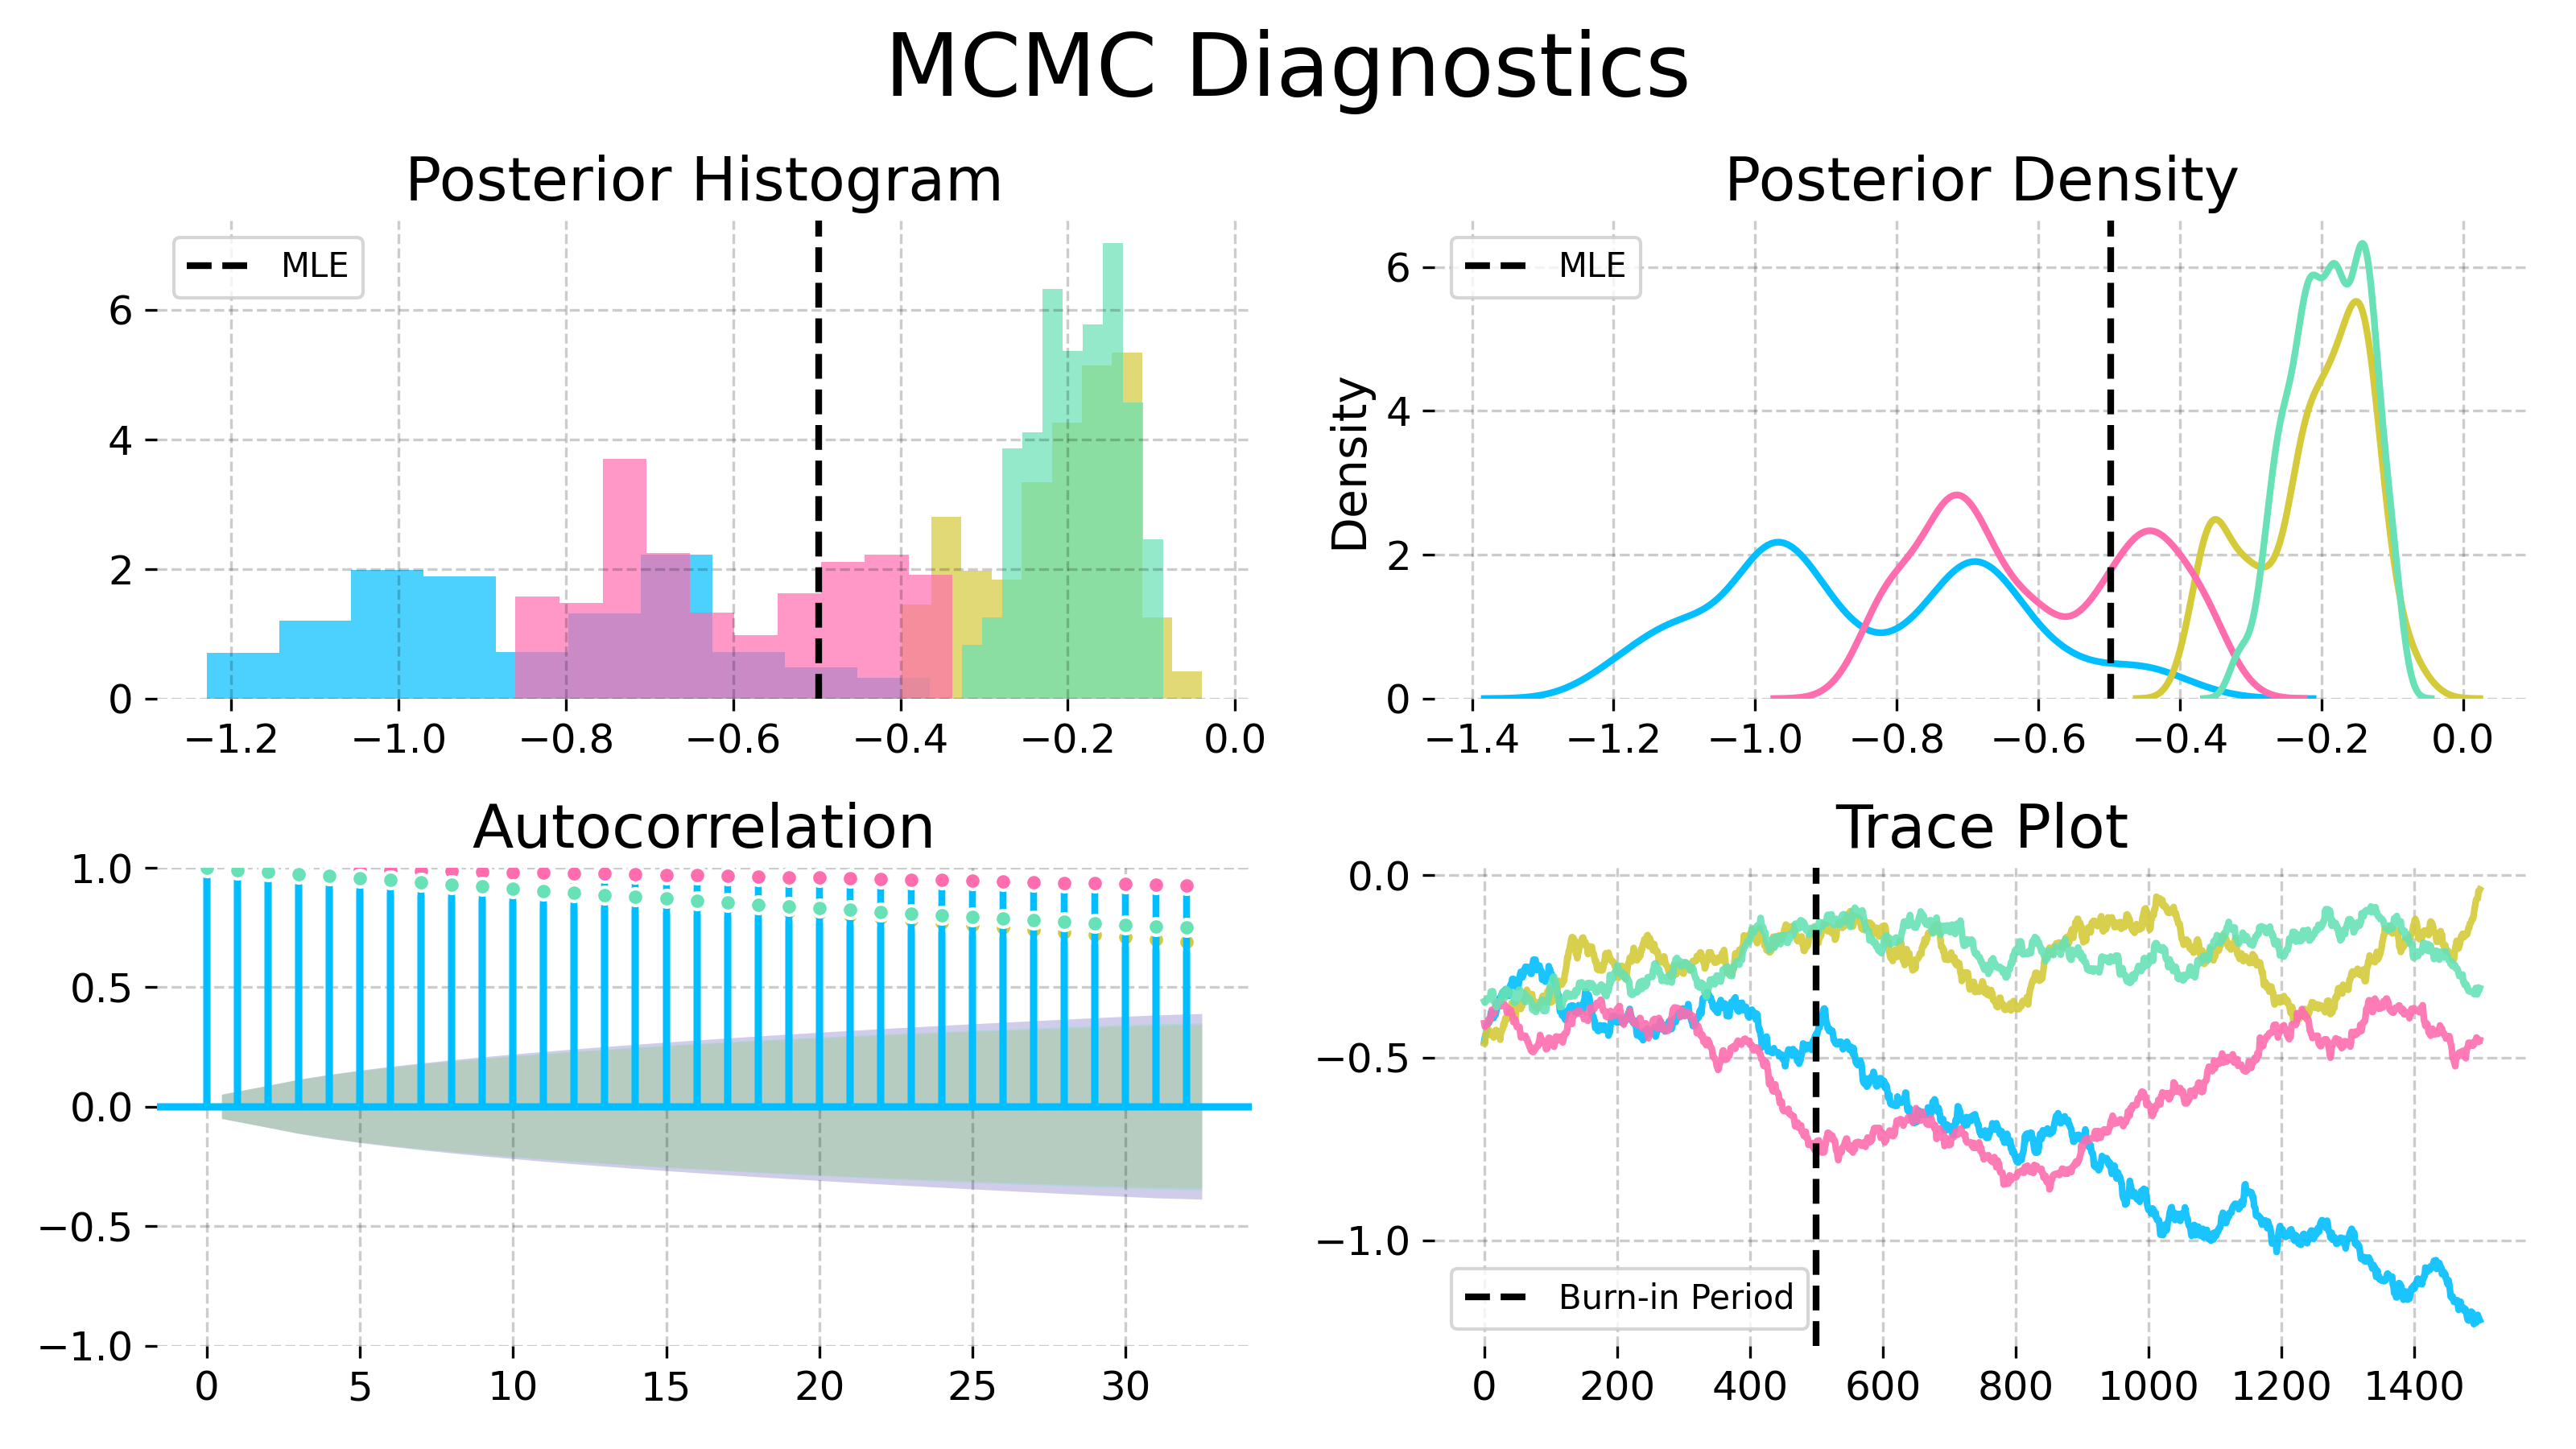
\includegraphics[width=0.76\textwidth]{figures/ch07/imgs/pmcmc/mh.png}
\caption{
  Convergence diagnostics for the Metropolis-Hastings variant particle MCMC with the random walk proposal and an informative empirical prior from IF2, on the trend parameter in the Dhaka cholera model of \cite{king08}.
  The poor convergence shown here, using an MCMC algorithm that does not have access to derivatives, contrasts with Fig.~{\refFigNutsEb} in the main text.
}
    \label{fig:mh}
\end{figure}
\FloatBarrier

%\newpage

\begin{figure}[H]
    \centering
    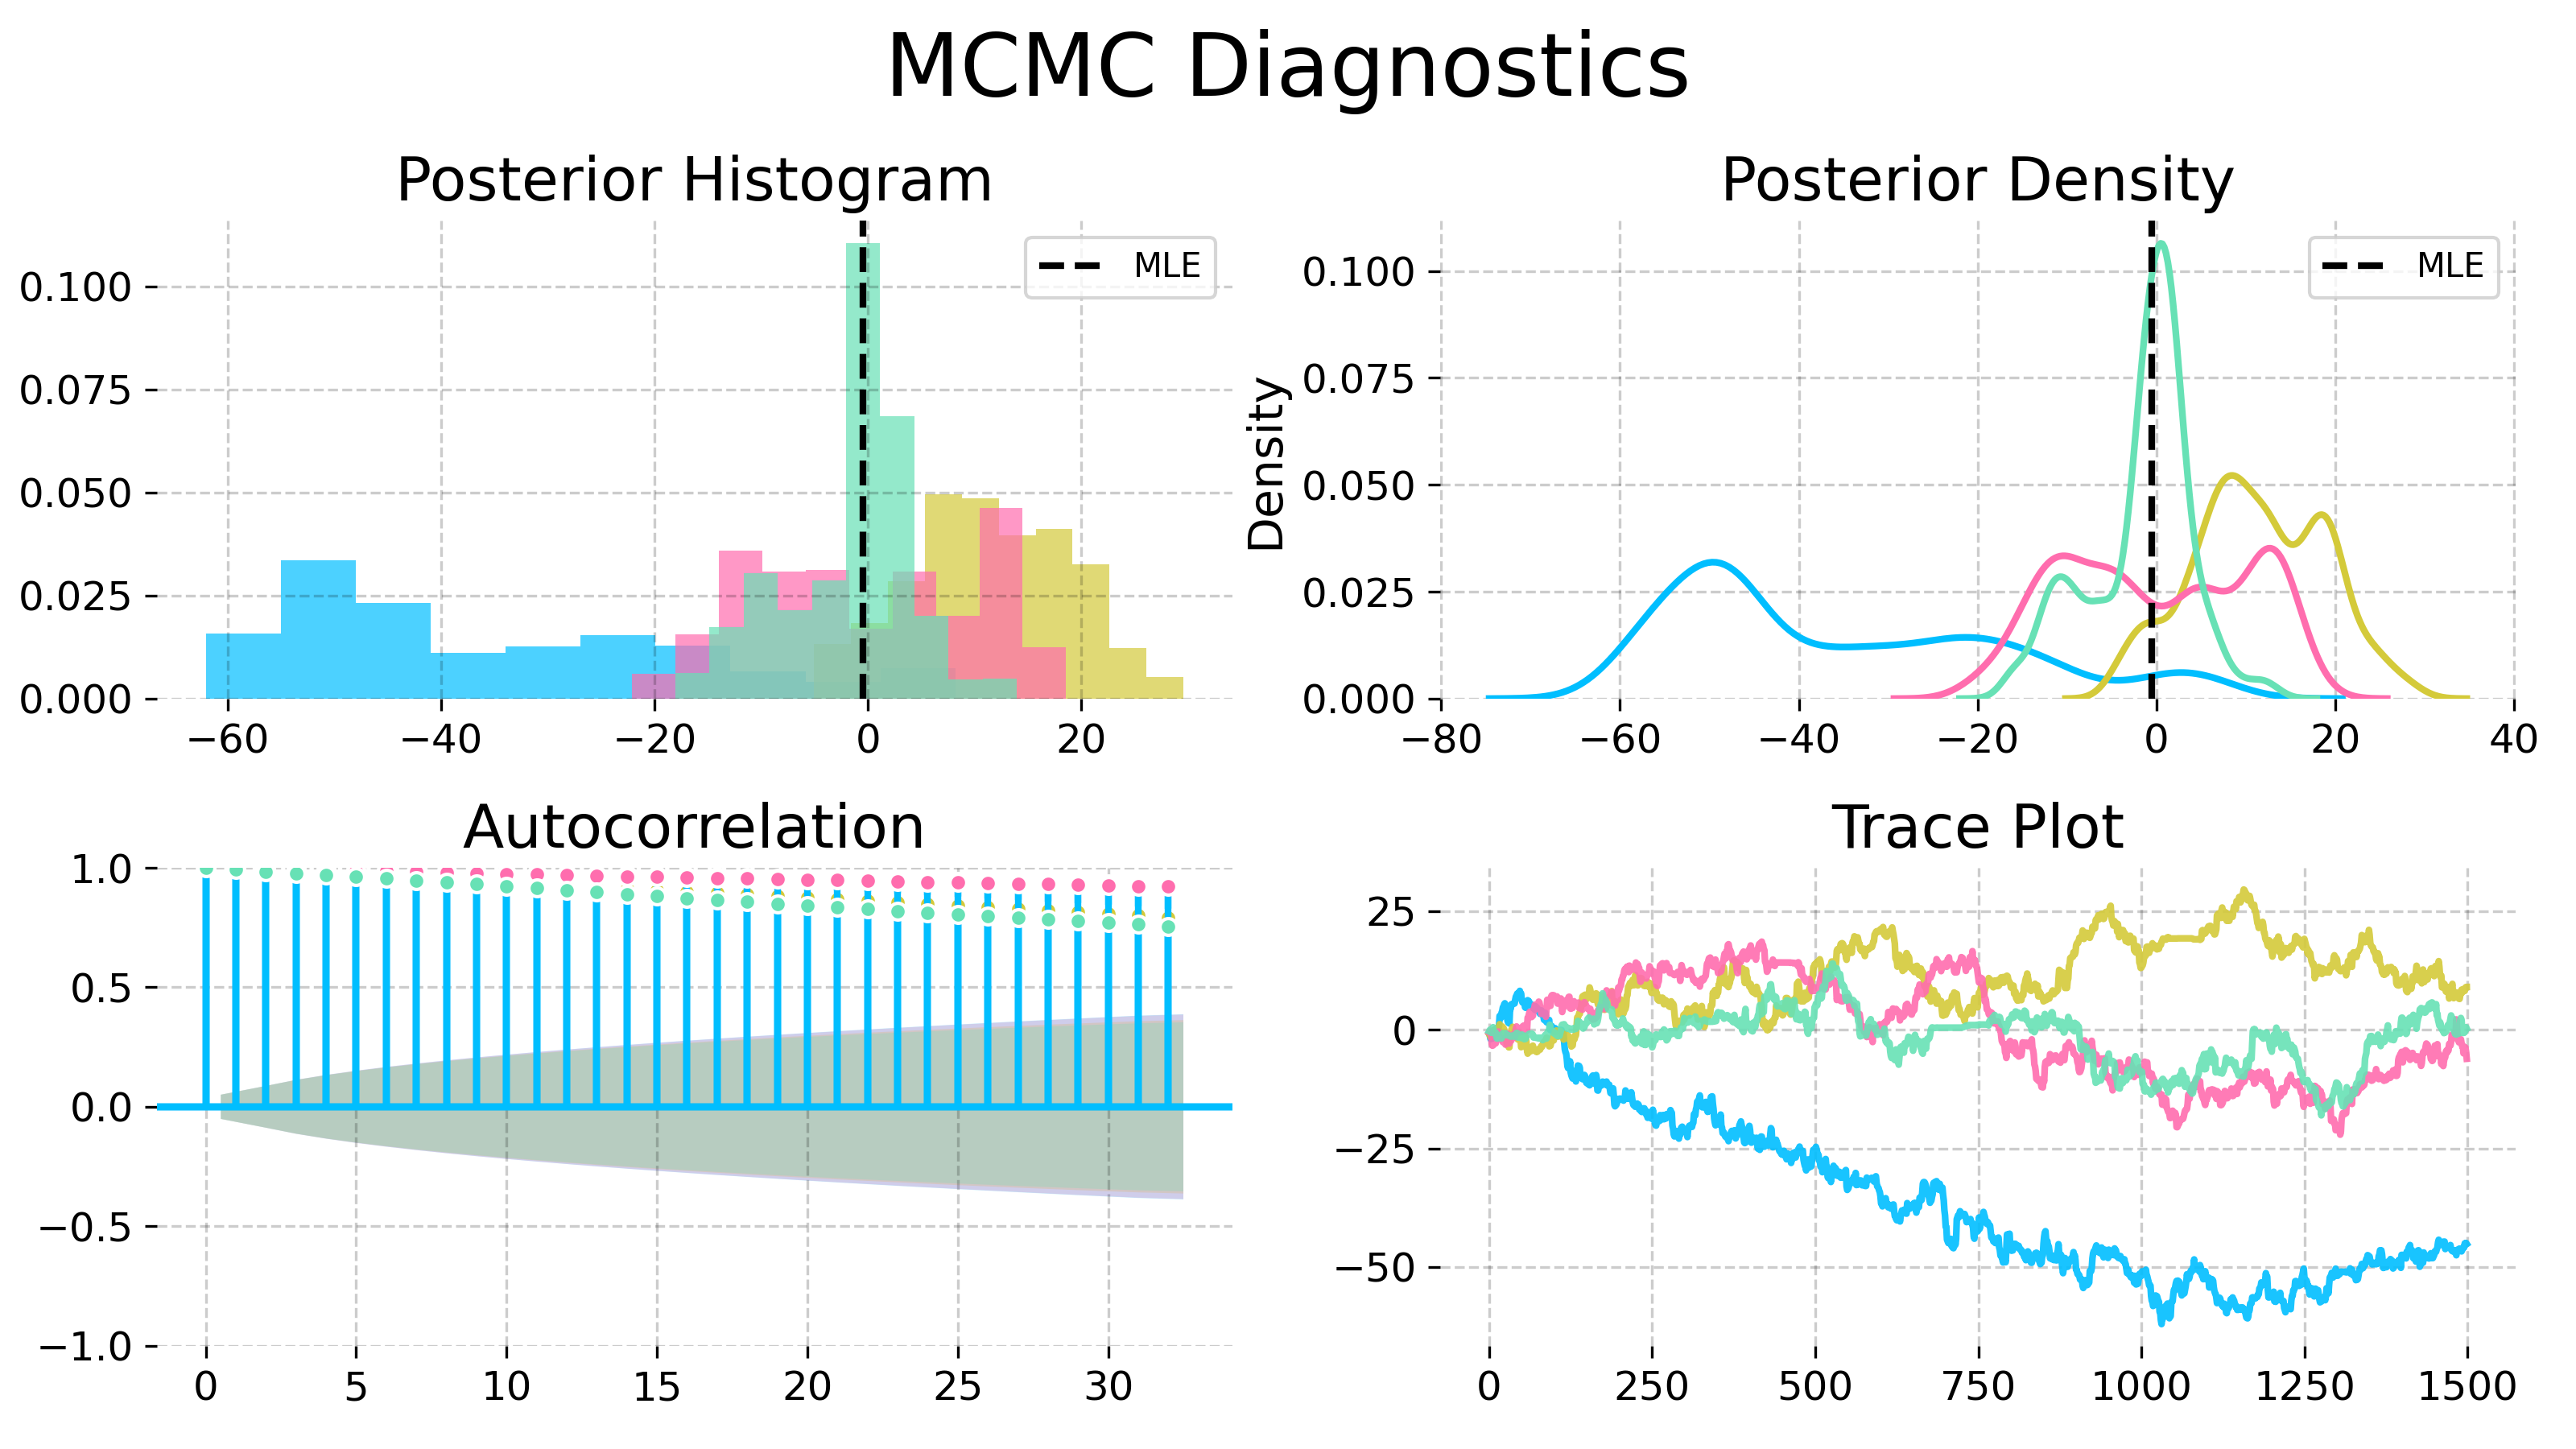
\includegraphics[width=0.76\textwidth]{figures/ch07/imgs/pmcmc/nuts.png}
    \caption{Convergence diagnostics for a No-U-Turn Sampler (NUTS) with uniform priors on a compact set, on the trend parameter in the Dhaka cholera model of \cite{king08}. The NUTS sampler explores more of the posterior than the Metropolis-Hastings sampler, but fails to converge quickly.
      This poor convergence, compared with Fig.~{\refFigNutsEb} in the main text, demonstrates the value of the empirical prior for obtaining successful convergence.
}
    \label{fig:nuts}
\end{figure}
\FloatBarrier
\newpage

\begin{figure}[H]
    \centering\
    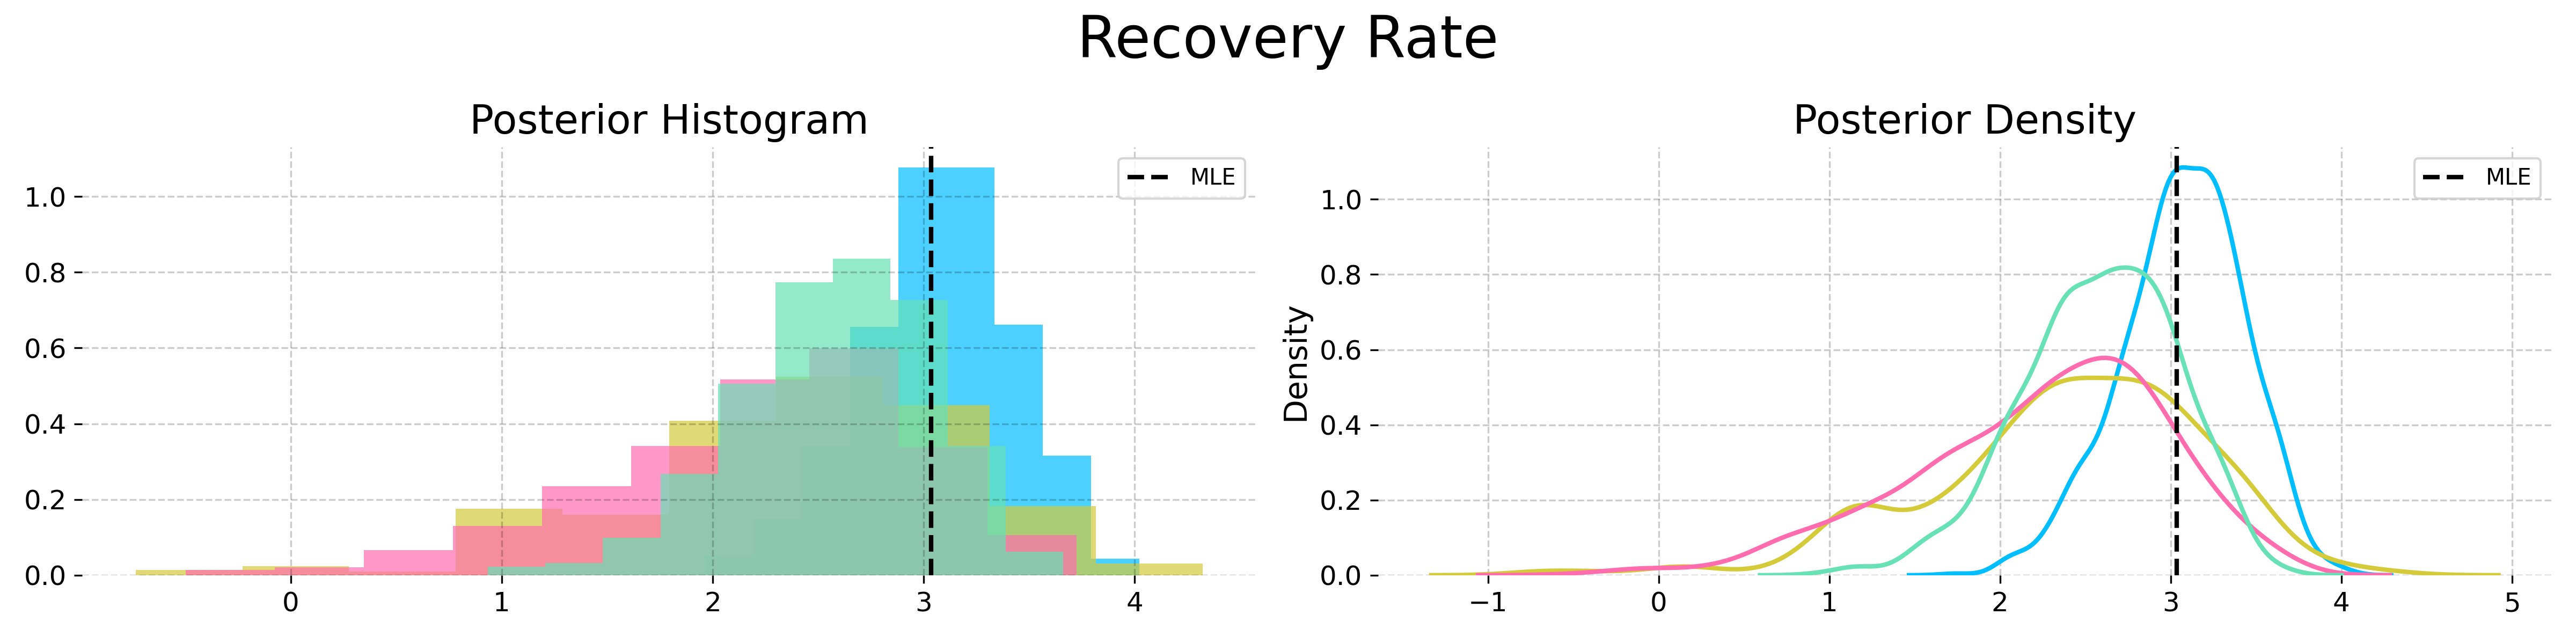
\includegraphics[scale=0.30]{figures/ch07/imgs/pmcmc/nuts_eb/Recovery_Rate.png}
    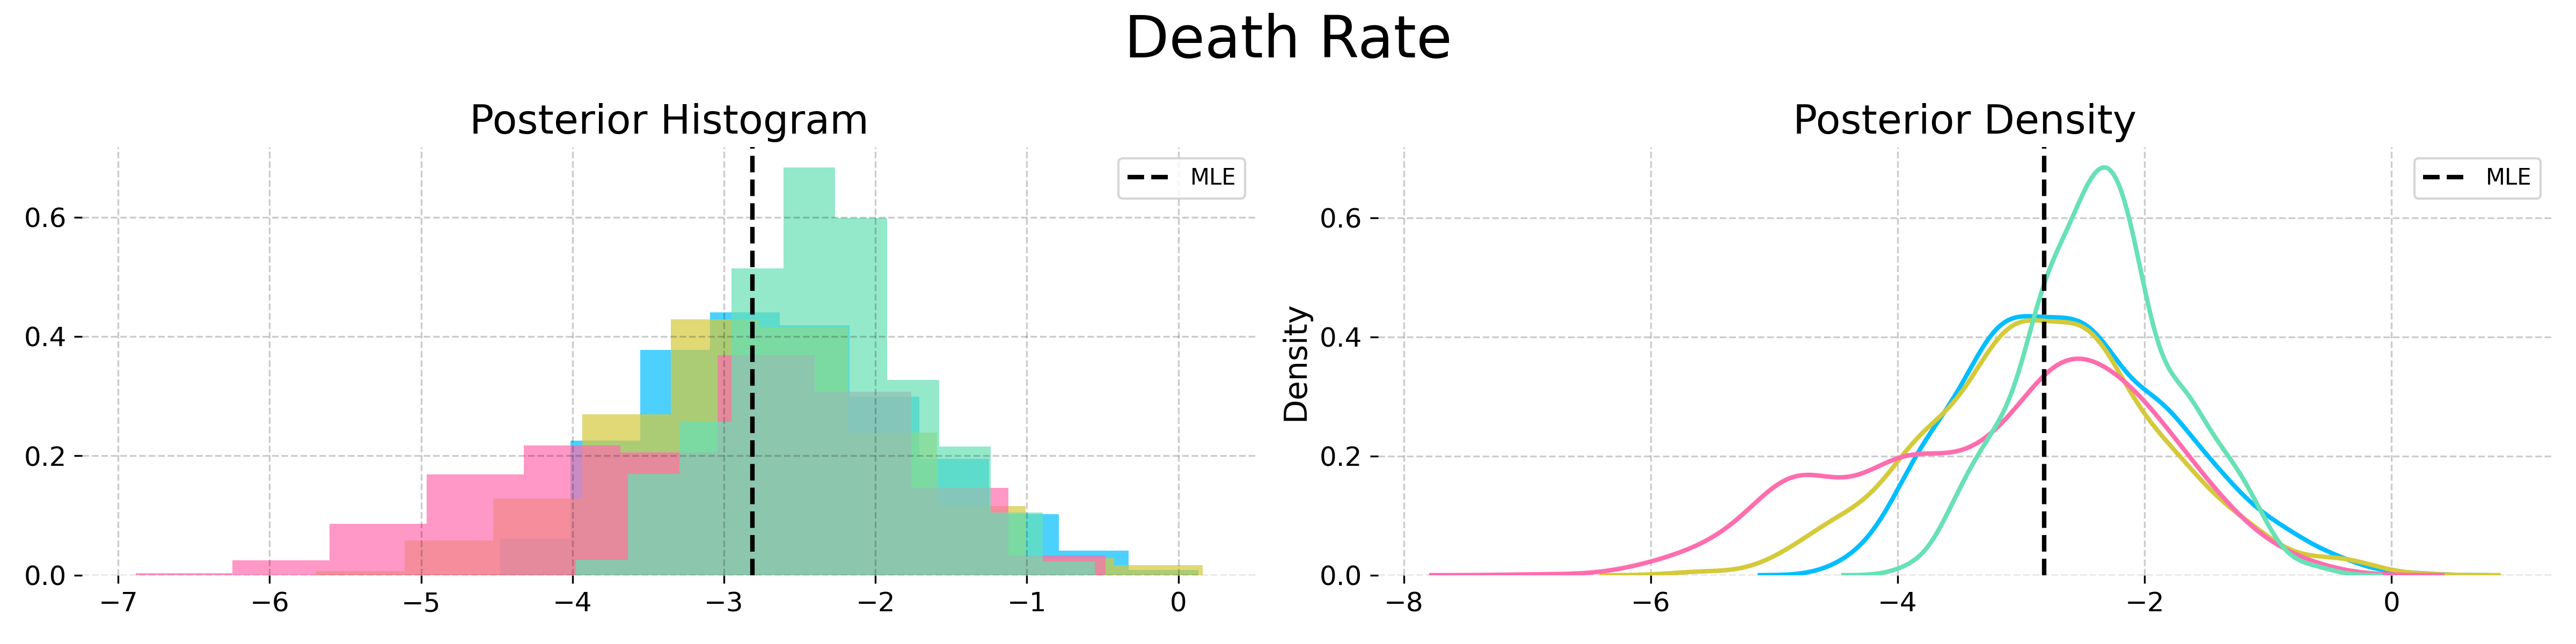
\includegraphics[scale=0.30]{figures/ch07/imgs/pmcmc/nuts_eb/Death_Rate.png}
    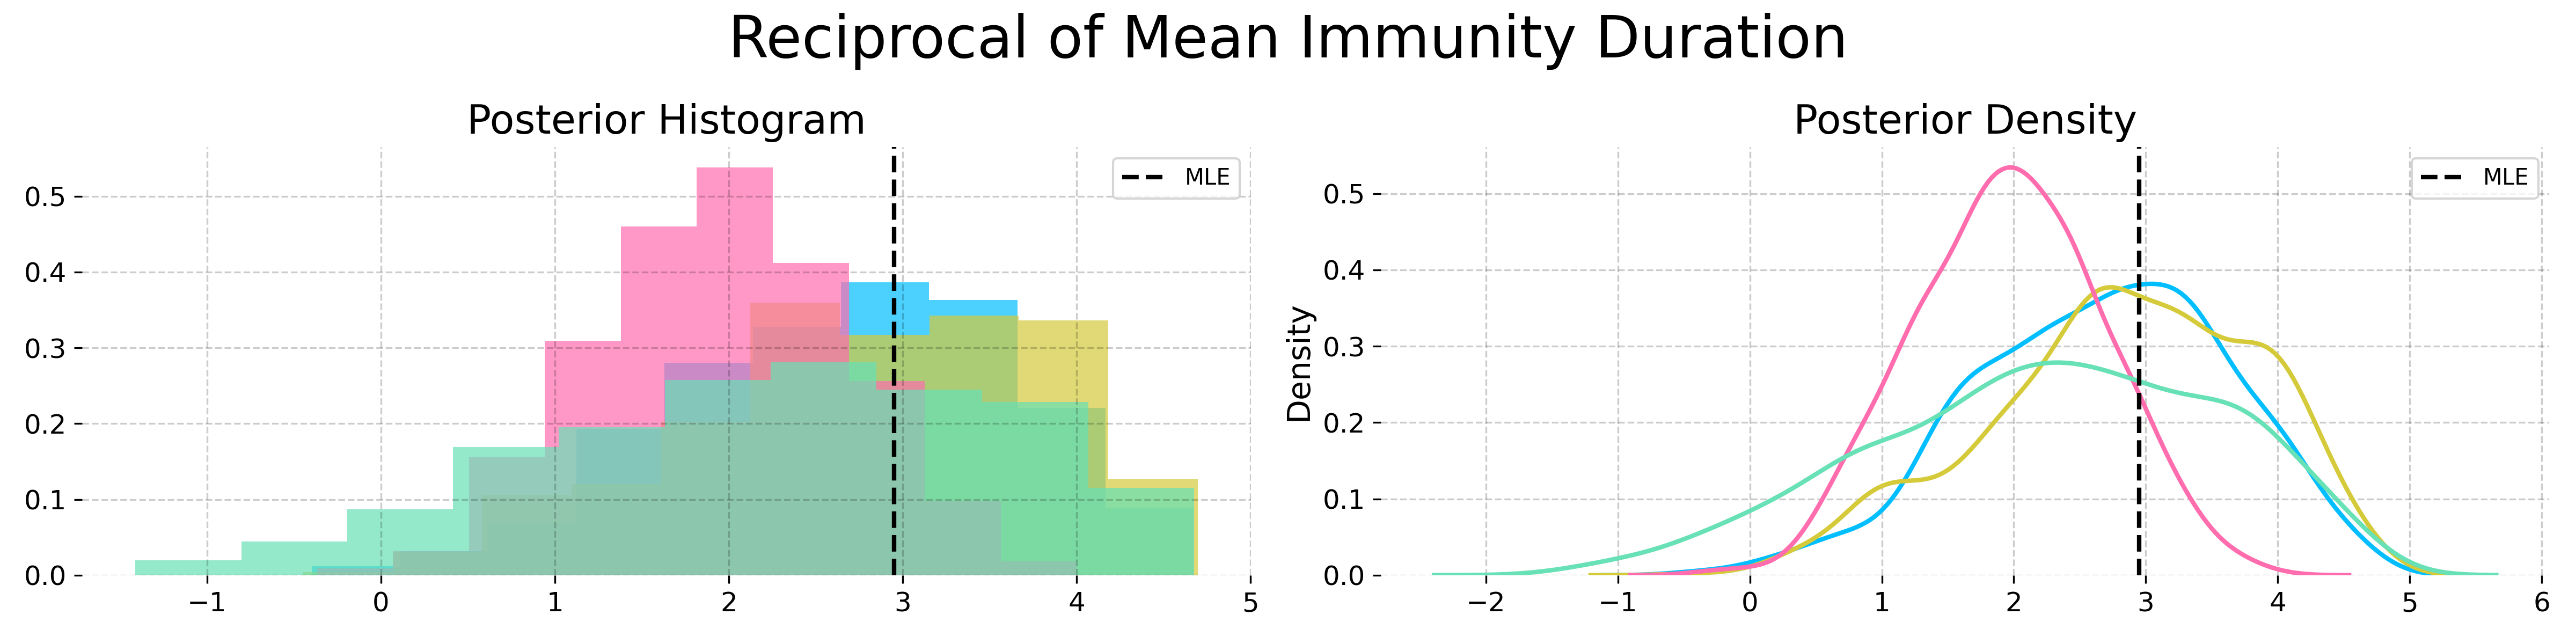
\includegraphics[scale=0.30]{figures/ch07/imgs/pmcmc/nuts_eb/Reciprocal_of_Mean_Immunity_Duration.png}
    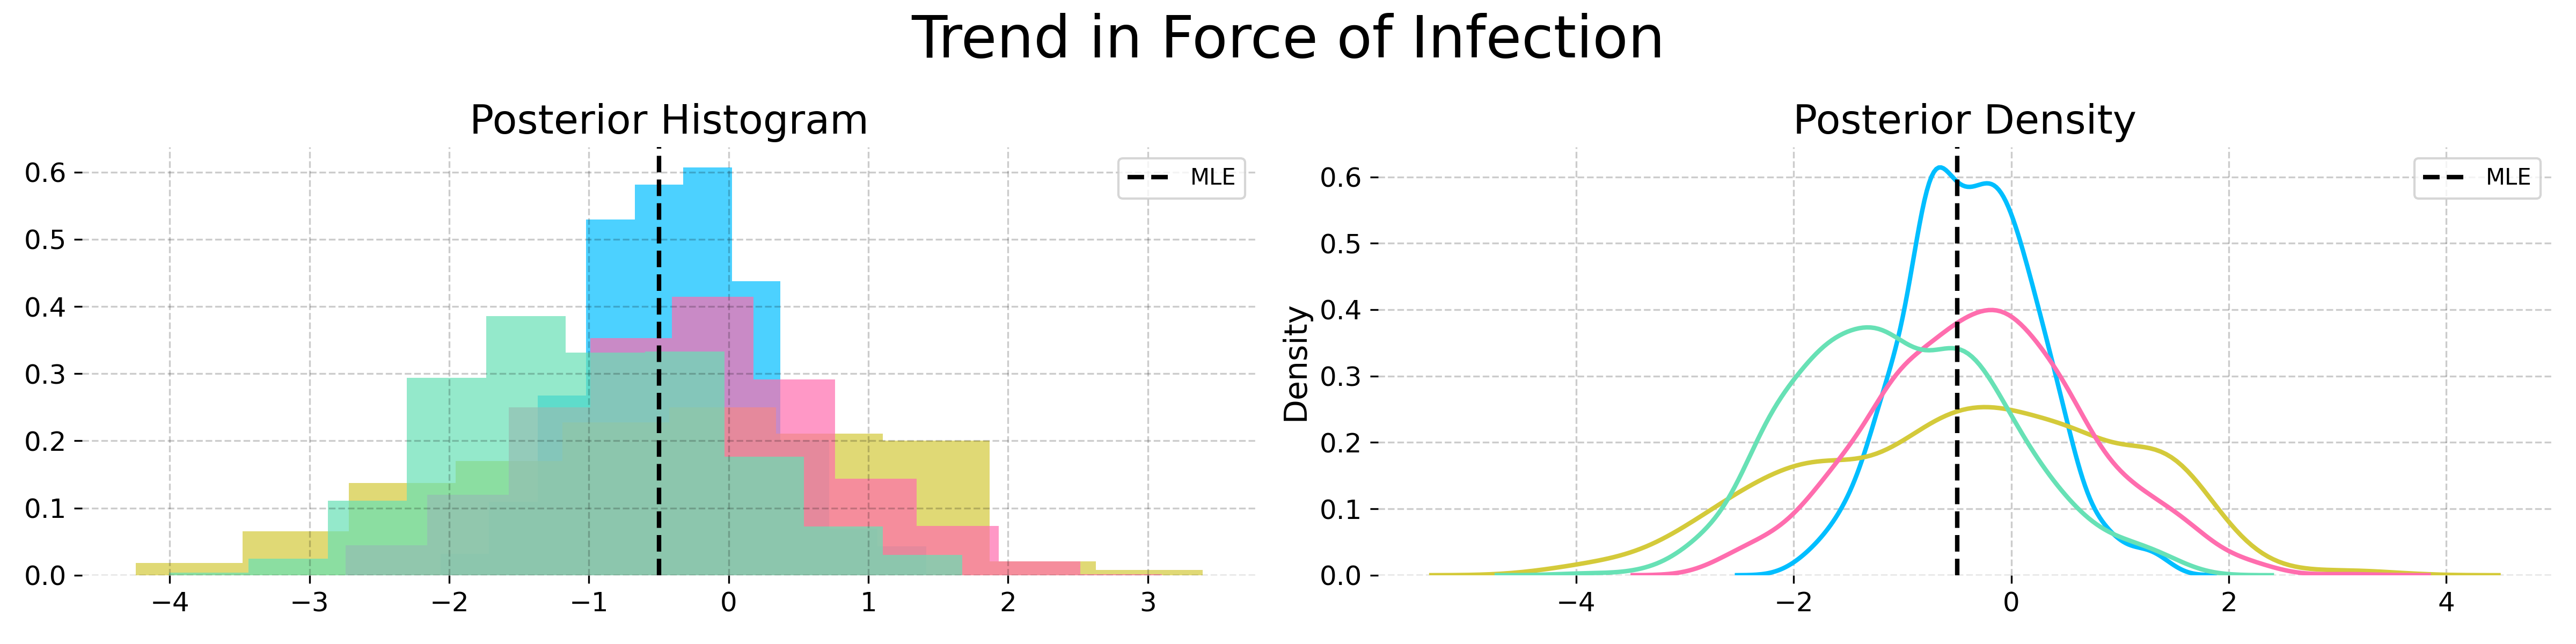
\includegraphics[scale=0.30]{figures/ch07/imgs/pmcmc/nuts_eb/Trend_in_Force_of_Infection.png}
    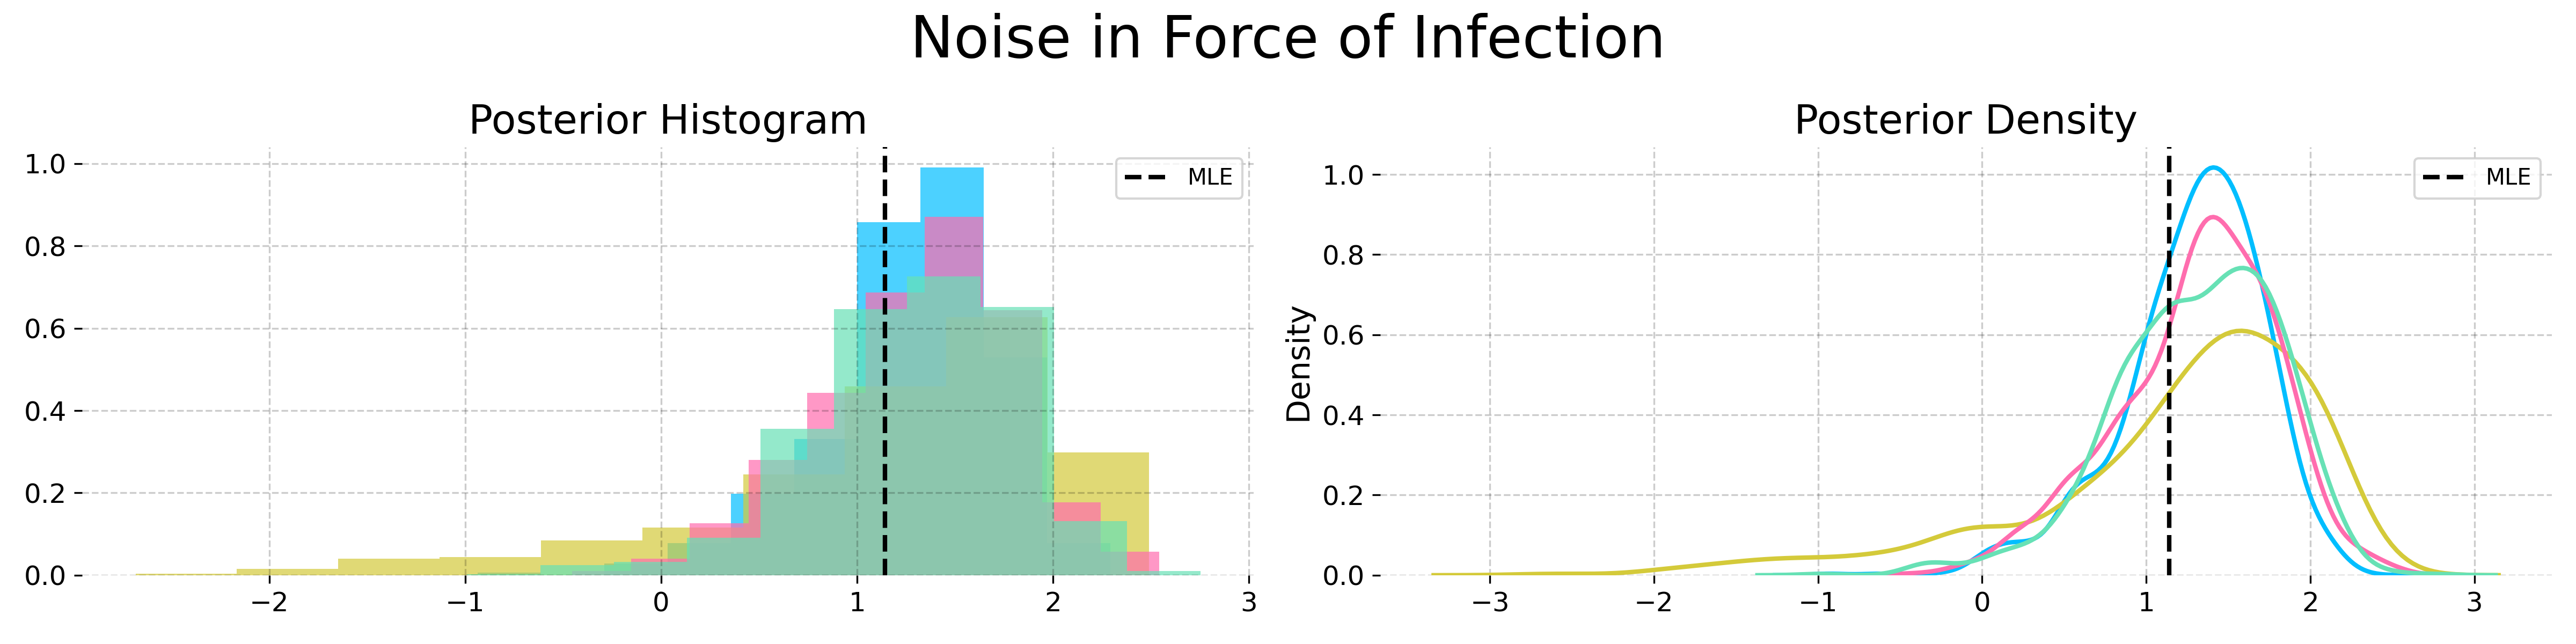
\includegraphics[scale=0.30]{figures/ch07/imgs/pmcmc/nuts_eb/Noise_in_Force_of_Infection.png}
    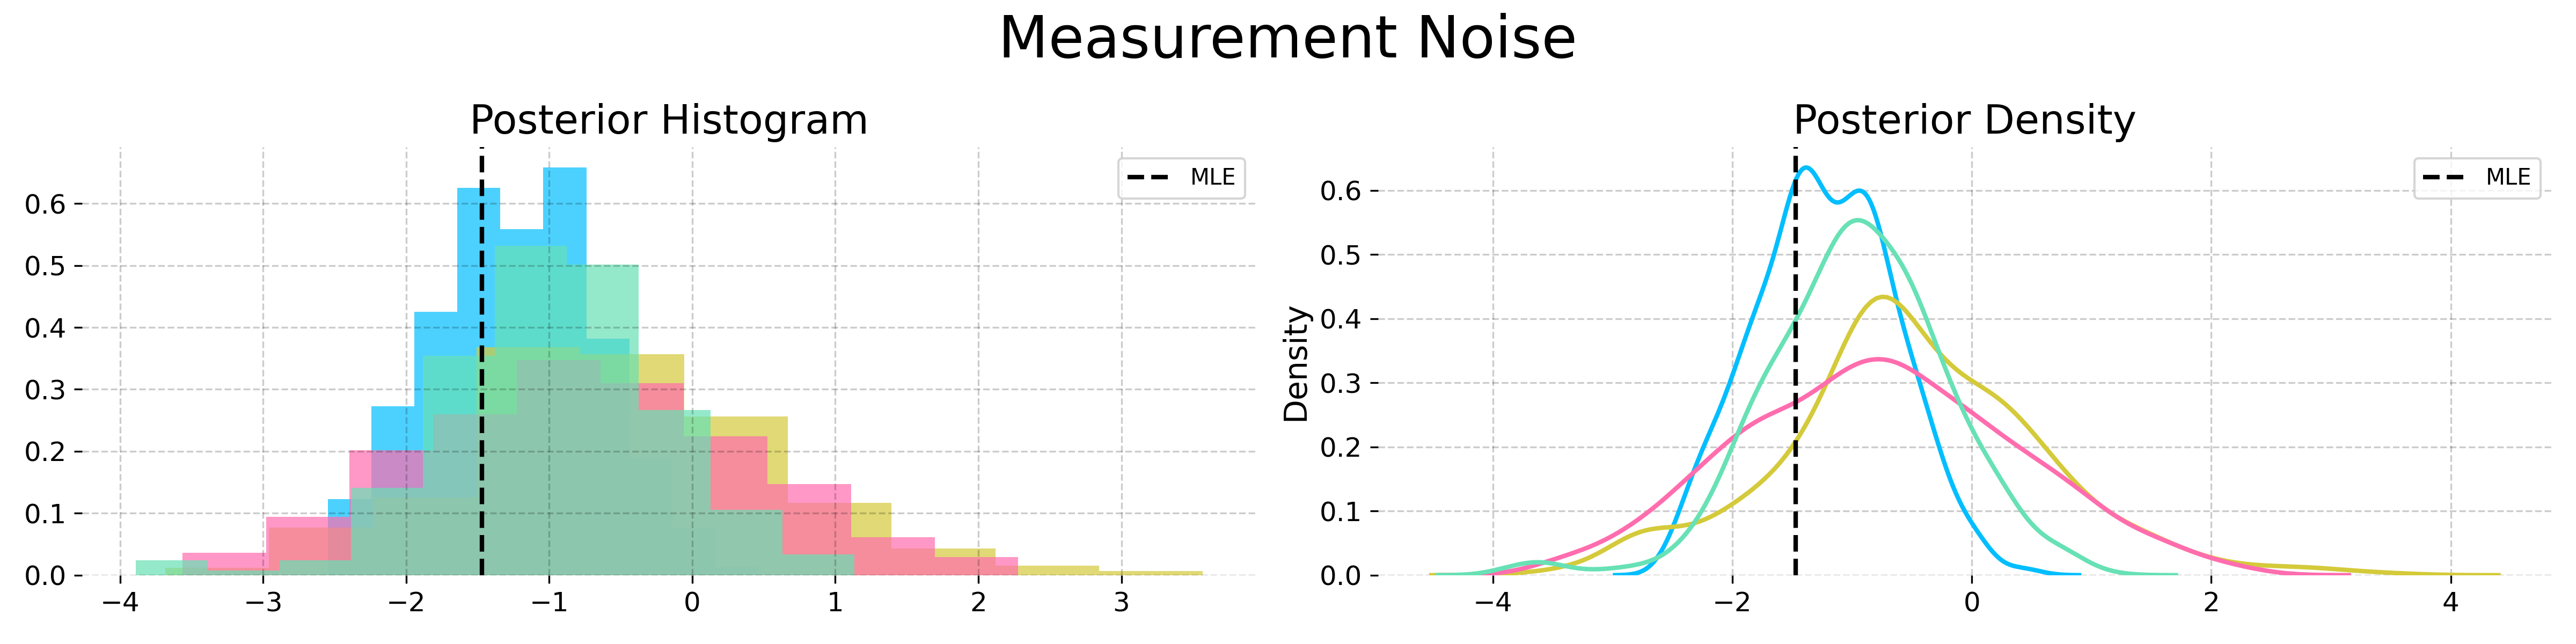
\includegraphics[scale=0.30]{figures/ch07/imgs/pmcmc/nuts_eb/Measurement_Noise.png}
    \caption{Posterior estimates from NUTS powered by \aigen{Algorithm~\ref{alg:mop}} with the informative nonparametric empirical prior obtained from a kernel density estimator on the IF2 parameter cloud. The posterior estimates from each chain are largely in agreement.}
    \label{fig:posteriors}
\end{figure}

\FloatBarrier
\newpage

\section{Algorithmic Parameters}
\label{sec:app07-s9}
\label{appendix:algparams}

We include the full set of algorithmic parameters used for the Dhaka results in Table~\ref{table:algparams}. 
The warm start iterations are IF2 iterations, which are followed by gradient descent (GD) iterations when using \aigen{Algorithm~\ref{alg:ifad}}. 
The IF2 cooling rate is the fractional reduction in the parameter perturbations over 50 iterations, so that a cooling rate of 0.5 corresponds to approximately 1\% cooling per iteration.
The random walk standard deviation (RWSD) scales the noise added at each filtering step to each regular parameter.
Initial value parameters (IVPs), that affect the value of the latent process only at time $t_0$, are treated differently: they are perturbed only at time $t_0$, with a larger RWSD. 
Parameters are transformed to a unit scale, for example by taking logarithms or a logistic transformation, so that a single RWSD value works for all parameters.

\begin{table}[H]
\centering
\resizebox{\linewidth}{!}{%
\begin{tabular}{p{4.5cm}cccc}
\toprule
\textbf{Hyperparameter} & \textbf{Standard IF2} & \textbf{\aigen{Alg.~\ref{alg:ifad} ($\alpha=0$)}} & \textbf{\aigen{Alg.~\ref{alg:ifad} ($\alpha=0.97$)}} & \textbf{\aigen{Alg.~\ref{alg:ifad} ($\alpha=1$)}} \\
\midrule
Number of Particles ($J$) & 5,000 & 5,000 & 5,000 & 5,000 \\
Warm-start Iterations & 1,950 & 60 & 175 & 60 \\
GD Iterations & --- & 410 & 400 & 425 \\
IF2 Cooling Rate & 0.93 & 0.5 & 0.5 & 0.5 \\
Initial RWSD & 0.02 & 0.02 & 0.02 & 0.02 \\
Initial RWSD (IVPs) & 0.16 & 0.16 & 0.16 & 0.16 \\
Gradient Optimizer & --- & Adam & Adam & Adam \\
Momentum ($\beta_1$) & --- & 0.0 & 0.9 & 0.9 \\
LR Schedule & --- & Cosine Decay & Cosine Decay & Cosine Decay \\
Initial LR ($\eta_0$) & --- & 0.1 & 0.1 & 0.1 \\
Warm-up Steps & --- & 10 & 10 & 10 \\
Eval. Particles / Reps & 5,000 / 36 & 5,000 / 36 & 5,000 / 36 & 5,000 / 36 \\
\bottomrule
\end{tabular}%
}
\caption{Algorithmic parameters for the global search benchmarking on the Dhaka cholera model.}
\label{table:algparams}
\end{table}

Following some experimentation, \aigen{Algorithm~\ref{alg:ifad}} was implemented by plugging the \aigen{Algorithm~\ref{alg:dmop}} gradient estimate into the Adam optimizer \citep{kingma15}.
The momentum parameter in Adam was turned off for \aigen{Algorithm~\ref{alg:ifad} ($\alpha=0$)}, since this low-variance estimate did not require it.
Decreasing the learning rate (LR) was found to be helpful, and we selected the commonly used cosine decay.
Warm-up steps were taken with Adam to stabilize its initial performance and avoid noisy 


\clearpage

\section{Application to a Daphnia Population Model}
\label{sec:app07-s10}
\label{sec:daphnia}

\subsection{Model and data}

The SIRJPF2 model developed by \citet{yang25daphnia} describes interactions between two species of \textit{Daphnia}, their algal food, and a fungal parasite.
We use the version with unit-specific infected-adult mortality to compare likelihood maximization by \aigen{Algorithm~\ref{alg:ifad}} and the marginalized panel iterated filter (MPIF) of \citet{wheeler25}.

The data come from the mesocosm experiment of \citet{searle16}.
We use the treatment containing the native species \textit{D.~dentifera}, the invasive species \textit{D.~lumholtzi}, and the parasite \textit{Metschnikowia bicuspidata}, with eight mesocosms, each treated as one unit in the panel.
Each mesocosm was observed at ten times, $t_n=5n+2$ days for $n=1,\ldots,10$.
At each observation time, a one-liter sample was taken and susceptible and infected adult females of both species were counted.
Juvenile counts are excluded from the likelihood.

We write $S_u^a(t)$, $I_u^a(t)$, and $J_u^a(t)$ for the densities of susceptible adult females, infected adult females, and juveniles, where $u=1,\ldots,8$ indexes the mesocosm and $a\in\{\mathrm n,\mathrm i\}$ denotes the native or invasive species.
The densities of food and parasite spores are $F_u(t)$ and $P_u(t)$.
These variables form an eight-dimensional latent state in each mesocosm.
Removal by death, consumption, or sampling is denoted by $R$ in the model name and does not require an additional state variable.
The two host species interact through their shared food and parasite populations.
The processes in different mesocosms are independent conditional on the parameters.

As in \citet{yang25daphnia}, the transition dynamics follow an It\^o stochastic differential equation (SDE):
\begin{align*}
dS_u^a
 &= \{\lambda_J J_u^a-(\theta_S^a+p^a f_S^aP_u+\delta)S_u^a\}\,dt
    +\sigma_S^a S_u^a\,dB_{S,u}^a,\\
dI_u^a
 &= \{p^a f_S^a S_u^aP_u-(\theta_{I,u}^a+\delta)I_u^a\}\,dt
    +\sigma_I^a I_u^a\,dB_{I,u}^a,\\
dJ_u^a
 &= \{r^a f_S^aF_uS_u^a-(\theta_J^a+\delta+\lambda_J)J_u^a\}\,dt
    +\sigma_J^a J_u^a\,dB_{J,u}^a,\\
dP_u
 &= \left\{\sum_a\left[\beta\theta_{I,u}^a I_u^a
          -f_S^a(S_u^a+\xi I_u^a)P_u\right]
          -(\theta_P+\delta)P_u\right\}\,dt
    +\sigma_P P_u\,dB_{P,u},\\
dF_u
 &= \left\{\mu-\delta F_u
          -\sum_a f_S^aF_u(S_u^a+\xi I_u^a+J_u^a)\right\}\,dt
    +\sigma_F F_u\,dB_{F,u},
\end{align*}
with independent standard Brownian motions $B$.
The time argument is suppressed in the equations.
Except for infected-adult mortality, estimated parameters are shared across mesocosms.
The parameters $r^a$ and $f_S^a$ are the reproductive rate and host filtration rate, $p^a$ controls infection following spore ingestion, and $\xi$ is the filtration rate of infected adults relative to susceptible adults.
The mortality or loss rates of susceptible adults, infected adults, juveniles, and spores are $\theta_S^a$, $\theta_{I,u}^a$, $\theta_J^a$, and $\theta_P$, respectively; the $\sigma$ parameters are process-noise coefficients.
The relative filtration rate of juveniles is fixed at one.

We use the units of the public Python implementation:\footnote{\href{https://github.com/pypomp/Daphnia-tutorial/blob/f3183301273a409e5b079bb0ae3a22246f69ba7a/Python-code/daphnia_tut_pypomp_advanced.qmd}{\texttt{pypomp/Daphnia-tutorial}, advanced tutorial, revision \texttt{f318330}.}}
\textit{Daphnia} densities are individuals per liter, $F$ is in $10^6$ algal cells per liter, and $P$ is in $10^3$ spores per liter, with parameters expressed in the corresponding units.
The sampling loss rate is fixed at $\delta=0.013$ per day, the food replenishment rate at $\mu=0.37$, the juvenile maturation rate at $\lambda_J=0.1$ per day, and the spore yield per infected-host death at $\beta=30$, corresponding to $3\times10^4$ spores.
The initial states are $S_u^{\mathrm n}=2.333$, $S_u^{\mathrm i}=0.667$, and $F_u=16.667$, with the remaining states set to zero.
Simulation begins at $t_0=1$ day, and parasites are introduced on day~4 at a density of $25\times10^3$ spores per liter.
We numerically solve the SDE using the Euler-Maruyama method with a time step of 0.25 days, following the initial conditions, inoculation, and numerical boundary rules of the public implementation.

The measurement model for the adult counts is
\[
Y_{S,u,n}^a\sim\operatorname{NBinomial}(S_u^a(t_n),\tau_S^a),
\qquad
Y_{I,u,n}^a\sim\operatorname{NBinomial}(I_u^a(t_n),\tau_I^a),
\]
where $\operatorname{NBinomial}(m,\tau)$ has mean $m$ and variance $m+m^2/\tau$ \citep{yang25daphnia}.
The four counts at each observation time are independent conditional on the latent state.
Since the sampled volume is one liter, the state densities and observed counts are on the same scale.
The numerical implementation sets a lower bound of $10^{-10}$ on the negative binomial mean and size parameters.
As in the public Python code, a state variable that crosses a numerical boundary is reset to zero, and that particle's log weight for the mesocosm at the next observation is set to $-150$.
The boundary thresholds and the treatment of the inoculation time are specified in the code.

We fix $\sigma_S^{\mathrm n}=\sigma_S^{\mathrm i}=0$ and estimate $\theta_{I,u}^{\mathrm n}$ and $\theta_{I,u}^{\mathrm i}$ separately for each mesocosm.
The remaining 22 estimated parameters are shared across mesocosms, giving $22+2\times8=38$ estimated parameters.
This is the model with unit-specific infected-adult mortality in Table~S3 of the archived revision \citep{yang26daphniacode}.

\subsection{Experimental settings}

We tested \aigen{Algorithm~\ref{alg:ifad}} with discount factors $\alpha=0$, $\alpha=0.97$, and $\alpha=1$ against MPIF using Pypomp 1.0.5 \citep{abkemeier25}.
For each method, we performed 50 searches from the same starting parameter vectors, generated by independent lognormal perturbations of the initial parameter vector in the public tutorial, with a standard deviation of 0.45 on the log scale.
All positive estimated parameters were optimized on the log scale.
Each \aigen{Algorithm~\ref{alg:ifad}} search used an MPIF warm start of 200 iterations followed by 200 iterations of the Adam optimizer \citep{kingma15}, using \aigen{Algorithm~\ref{alg:dmop}} gradient estimates.
We ran MPIF alone for 680 iterations, chosen to approximate the computing time of \aigen{Algorithm~\ref{alg:ifad}}; measured times are reported in Table~\ref{tab:daphnia-results}.

We used 1,000 particles per mesocosm during optimization.
The initial random walk standard deviation (RWSD) for MPIF was 0.05 on the log scale, with geometric cooling by a factor of 0.7 over 50 iterations.
Adam used $\beta_1=0.9$, $\beta_2=0.999$, and $\epsilon=10^{-8}$, with all eight mesocosms contributing to each update.
The learning-rate schedule used ten steps of linear warmup multiplied by cosine decay with a final factor of 0.1.
A summary of the algorithmic parameters is provided in Table~\ref{tab:daphnia-settings}.

The learning-rate scale was selected using four additional starting points, separate from the 50 used for the comparison.
We compared the six combinations of learning-rate scales $0.001$, $0.005$, and $0.01$ with $\alpha\in\{0.9,0.97\}$.
The combination with the highest median final log-likelihood, evaluated by independent particle filtering, was $0.01$ with $\alpha=0.97$.
We used the same learning-rate schedule for $\alpha=0$ and $\alpha=1$.

\begin{table}[htbp!]
\centering
\resizebox{\linewidth}{!}{%
\begin{tabular}{p{4.5cm}cccc}
\toprule
\textbf{Hyperparameter} & \textbf{MPIF} & \textbf{\aigen{Alg.~\ref{alg:ifad} ($\alpha=0$)}} & \textbf{\aigen{Alg.~\ref{alg:ifad} ($\alpha=0.97$)}} & \textbf{\aigen{Alg.~\ref{alg:ifad} ($\alpha=1$)}} \\
\midrule
Particles per mesocosm ($J$) & 1,000 & 1,000 & 1,000 & 1,000 \\
MPIF Iterations & 680 & 200 & 200 & 200 \\
Adam Iterations & --- & 200 & 200 & 200 \\
MPIF Cooling Factor & 0.7 & 0.7 & 0.7 & 0.7 \\
Initial RWSD (log scale) & 0.05 & 0.05 & 0.05 & 0.05 \\
Momentum ($\beta_1$) & --- & 0.9 & 0.9 & 0.9 \\
Learning-rate Scale & --- & 0.01 & 0.01 & 0.01 \\
Warm-up Steps & --- & 10 & 10 & 10 \\
Eval. Particles / Reps & 2,000 / 10 & 2,000 / 10 & 2,000 / 10 & 2,000 / 10 \\
\bottomrule
\end{tabular}%
}
\caption{Algorithmic parameters for the Daphnia experiment. Particle numbers are per mesocosm; the cooling factor is the multiplier over 50 iterations.}
\label{tab:daphnia-settings}
\end{table}

All reported log-likelihoods were evaluated independently of optimization using ordinary particle filters, with 2,000 particles per mesocosm and ten replicates.
Likelihood estimates were averaged within each mesocosm before taking logarithms, and the eight mesocosm log-likelihoods were then summed.
Each method's best parameter vector was then held fixed and re-evaluated with ten fresh replicates at the same particle count, using the same model and Pypomp version on a CPU.
The same evaluation method was used for the final results and for intermediate saved parameter vectors.
The progress plot uses 25, 27, 26, and 22 saved parameter vectors per search for \aigen{Algorithm~\ref{alg:ifad} ($\alpha=0$)}, \aigen{Algorithm~\ref{alg:ifad} ($\alpha=0.97$)}, \aigen{Algorithm~\ref{alg:ifad} ($\alpha=1$)}, and MPIF, respectively, including the final evaluations.
Time is assigned in proportion to iteration number within each stage, using the measured total optimization time for that stage.
Each set of 50 searches ran on one Tesla V100 16 GB GPU, with two searches per batch.
Optimization times are summed over the 25 batches and include initial compilation but exclude the additional particle filter evaluations.

\subsection{Results}

Our findings are summarized in Table~\ref{tab:daphnia-results} and Figures~\ref{fig:daphnia-progress} and~\ref{fig:daphnia-raincloud}.
\aigen{Algorithm~\ref{alg:ifad} ($\alpha=0.97$)} and \aigen{Algorithm~\ref{alg:ifad} ($\alpha=1$)} attained maximum log-likelihoods of $-858.48$ and $-858.27$, respectively, each with a Monte Carlo standard error (MCSE) of approximately 0.17.
The maximum for MPIF was $-860.06$, with MCSE 0.16.
\aigen{Algorithm~\ref{alg:ifad} ($\alpha=0$)} attained $-860.36$ and had a median log-likelihood close to that of MPIF.

\begin{table}[htbp!]
\centering
\resizebox{\linewidth}{!}{%
\begin{tabular}{lrrrrr}
\toprule
 & Maximum & Re-evaluated & Median & MPIF time (s) & \aigen{AD stage} time (s) \\
\midrule
\aigen{Algorithm~\ref{alg:ifad} ($\alpha=0.97$)} & $-858.48\;(0.17)$ & $-858.23\;(0.16)$ & $-861.42$ & 535 & 1,309 \\
\aigen{Algorithm~\ref{alg:ifad} ($\alpha=1$)} & $-858.27\;(0.17)$ & $-858.00\;(0.14)$ & $-861.46$ & 520 & 1,313 \\
\aigen{Algorithm~\ref{alg:ifad} ($\alpha=0$)} & $-860.36\;(0.24)$ & $-860.30\;(0.21)$ & $-864.12$ & 503 & 1,314 \\
MPIF & $-860.06\;(0.16)$ & $-860.26\;(0.14)$ & $-864.27$ & 1,591 & - \\
\bottomrule
\end{tabular}%
}

\caption{Log-likelihoods from 50 searches per method, with MCSEs in parentheses. Re-evaluated uses fresh particle filters at each method's original maximizing parameter vector.}
\label{tab:daphnia-results}
\end{table}

Comparing searches from the same starting points, \aigen{Algorithm~\ref{alg:ifad} ($\alpha=0.97$)} and \aigen{Algorithm~\ref{alg:ifad} ($\alpha=1$)} each attained a higher final log-likelihood than MPIF in 49 of the 50 searches.
The median paired differences were 2.86 and 2.79 log-likelihood units, respectively.
The distributions of the final log-likelihoods for \aigen{Algorithm~\ref{alg:ifad} ($\alpha=0.97$)} and \aigen{Algorithm~\ref{alg:ifad} ($\alpha=1$)} were similar, which may be due to the short time series in each mesocosm.

\citet{yang26daphniacode} report a maximum log-likelihood of $-863.03$ in the revised Table~S3.
Our MPIF searches attained a higher value, and \aigen{Algorithm~\ref{alg:ifad} ($\alpha=0.97$)} and \aigen{Algorithm~\ref{alg:ifad} ($\alpha=1$)} improved on this further.

\begin{figure}[htbp!]
\centering
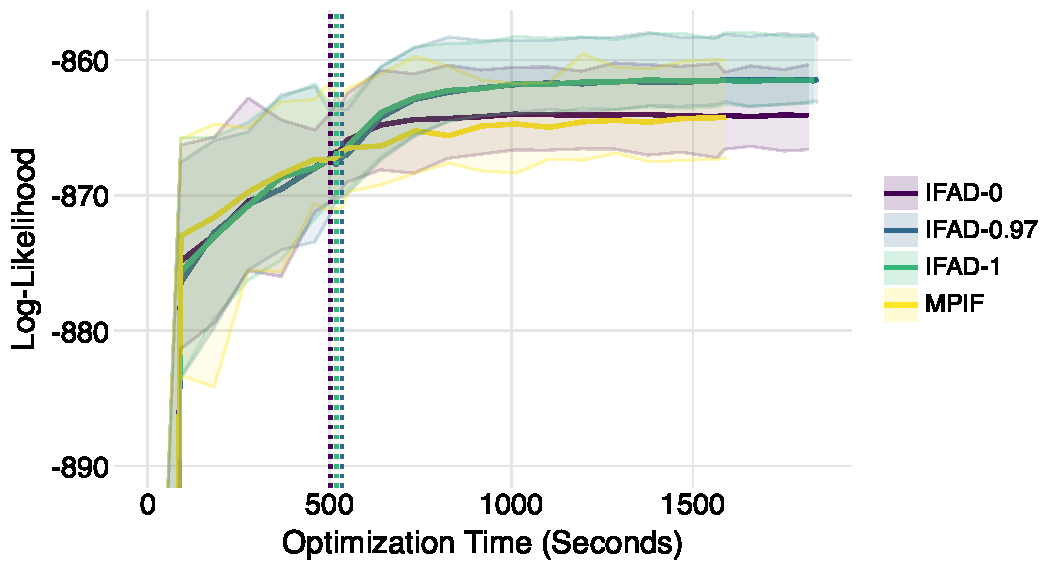
\includegraphics[width=0.95\textwidth]{figures/ch07/imgs/daphnia/daphnia_figure5.pdf}
\caption{Optimization progress of \aigen{Algorithm~\ref{alg:ifad}} and MPIF for the Daphnia model.
The solid lines show the median log-likelihood across 50 searches, and the shaded regions cover the area between the 10th and 100th percentiles.
The vertical dotted lines indicate where the \aigen{Algorithm~\ref{alg:ifad}} searches switch from MPIF to Adam optimization.
The plot shows log-likelihoods above $-890$; all searches contribute to the percentiles.}
\label{fig:daphnia-progress}
\end{figure}

\begin{figure}[htbp!]
\centering
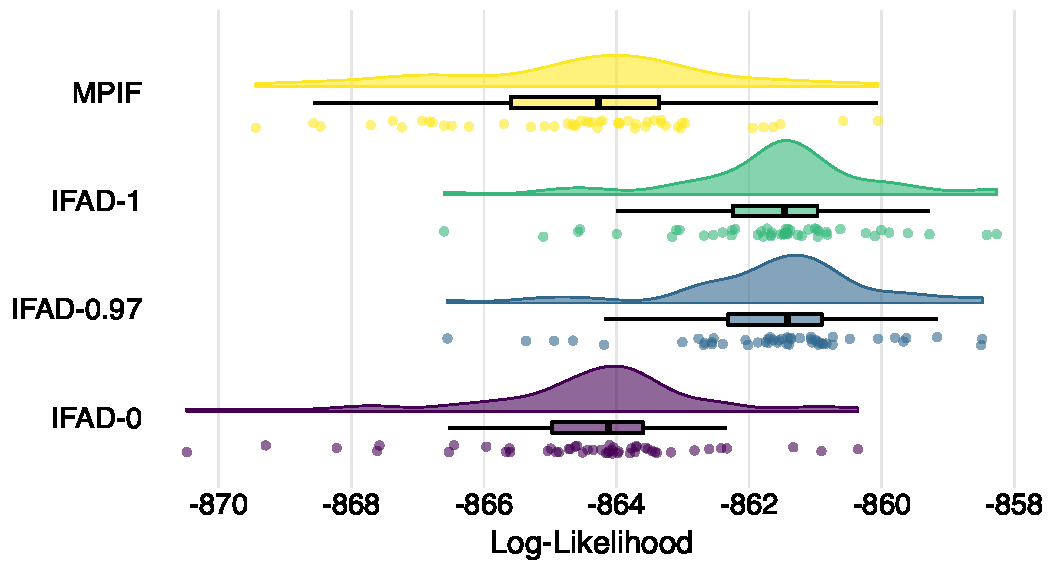
\includegraphics[width=0.95\textwidth]{figures/ch07/imgs/daphnia/daphnia_violin.pdf}
\caption{Raincloud plot of the searches for the Daphnia model.
The half-violin plots show the distributions of all 50 final log-likelihood estimates for each method, the boxplots show the medians and quartiles, and each point represents one search.
\aigen{Algorithm~\ref{alg:ifad} ($\alpha=0.97$)} and \aigen{Algorithm~\ref{alg:ifad} ($\alpha=1$)} have similar distributions, with generally higher log-likelihoods than MPIF and \aigen{Algorithm~\ref{alg:ifad} ($\alpha=0$)}.}
\label{fig:daphnia-raincloud}
\end{figure}

\clearpage



